% Options for packages loaded elsewhere
\PassOptionsToPackage{unicode}{hyperref}
\PassOptionsToPackage{hyphens}{url}
\PassOptionsToPackage{dvipsnames,svgnames,x11names}{xcolor}
%
\documentclass[
  letterpaper,
]{book}

\usepackage{amsmath,amssymb}
\usepackage{iftex}
\ifPDFTeX
  \usepackage[T1]{fontenc}
  \usepackage[utf8]{inputenc}
  \usepackage{textcomp} % provide euro and other symbols
\else % if luatex or xetex
  \usepackage{unicode-math}
  \defaultfontfeatures{Scale=MatchLowercase}
  \defaultfontfeatures[\rmfamily]{Ligatures=TeX,Scale=1}
\fi
\usepackage{lmodern}
\ifPDFTeX\else  
    % xetex/luatex font selection
\fi
% Use upquote if available, for straight quotes in verbatim environments
\IfFileExists{upquote.sty}{\usepackage{upquote}}{}
\IfFileExists{microtype.sty}{% use microtype if available
  \usepackage[]{microtype}
  \UseMicrotypeSet[protrusion]{basicmath} % disable protrusion for tt fonts
}{}
\makeatletter
\@ifundefined{KOMAClassName}{% if non-KOMA class
  \IfFileExists{parskip.sty}{%
    \usepackage{parskip}
  }{% else
    \setlength{\parindent}{0pt}
    \setlength{\parskip}{6pt plus 2pt minus 1pt}}
}{% if KOMA class
  \KOMAoptions{parskip=half}}
\makeatother
\usepackage{xcolor}
\usepackage[paperheight=257mm,paperwidth=188mm,top=25mm,headsep=10mm,bottom=30mm,footskip=15mm,left=25mm,right=25mm,centering]{geometry}
\setlength{\emergencystretch}{3em} % prevent overfull lines
\setcounter{secnumdepth}{2}
% Make \paragraph and \subparagraph free-standing
\ifx\paragraph\undefined\else
  \let\oldparagraph\paragraph
  \renewcommand{\paragraph}[1]{\oldparagraph{#1}\mbox{}}
\fi
\ifx\subparagraph\undefined\else
  \let\oldsubparagraph\subparagraph
  \renewcommand{\subparagraph}[1]{\oldsubparagraph{#1}\mbox{}}
\fi

\usepackage{color}
\usepackage{fancyvrb}
\newcommand{\VerbBar}{|}
\newcommand{\VERB}{\Verb[commandchars=\\\{\}]}
\DefineVerbatimEnvironment{Highlighting}{Verbatim}{commandchars=\\\{\}}
% Add ',fontsize=\small' for more characters per line
\usepackage{framed}
\definecolor{shadecolor}{RGB}{241,243,245}
\newenvironment{Shaded}{\begin{snugshade}}{\end{snugshade}}
\newcommand{\AlertTok}[1]{\textcolor[rgb]{0.68,0.00,0.00}{#1}}
\newcommand{\AnnotationTok}[1]{\textcolor[rgb]{0.37,0.37,0.37}{#1}}
\newcommand{\AttributeTok}[1]{\textcolor[rgb]{0.40,0.45,0.13}{#1}}
\newcommand{\BaseNTok}[1]{\textcolor[rgb]{0.68,0.00,0.00}{#1}}
\newcommand{\BuiltInTok}[1]{\textcolor[rgb]{0.00,0.23,0.31}{#1}}
\newcommand{\CharTok}[1]{\textcolor[rgb]{0.13,0.47,0.30}{#1}}
\newcommand{\CommentTok}[1]{\textcolor[rgb]{0.37,0.37,0.37}{#1}}
\newcommand{\CommentVarTok}[1]{\textcolor[rgb]{0.37,0.37,0.37}{\textit{#1}}}
\newcommand{\ConstantTok}[1]{\textcolor[rgb]{0.56,0.35,0.01}{#1}}
\newcommand{\ControlFlowTok}[1]{\textcolor[rgb]{0.00,0.23,0.31}{\textbf{#1}}}
\newcommand{\DataTypeTok}[1]{\textcolor[rgb]{0.68,0.00,0.00}{#1}}
\newcommand{\DecValTok}[1]{\textcolor[rgb]{0.68,0.00,0.00}{#1}}
\newcommand{\DocumentationTok}[1]{\textcolor[rgb]{0.37,0.37,0.37}{\textit{#1}}}
\newcommand{\ErrorTok}[1]{\textcolor[rgb]{0.68,0.00,0.00}{#1}}
\newcommand{\ExtensionTok}[1]{\textcolor[rgb]{0.00,0.23,0.31}{#1}}
\newcommand{\FloatTok}[1]{\textcolor[rgb]{0.68,0.00,0.00}{#1}}
\newcommand{\FunctionTok}[1]{\textcolor[rgb]{0.28,0.35,0.67}{#1}}
\newcommand{\ImportTok}[1]{\textcolor[rgb]{0.00,0.46,0.62}{#1}}
\newcommand{\InformationTok}[1]{\textcolor[rgb]{0.37,0.37,0.37}{#1}}
\newcommand{\KeywordTok}[1]{\textcolor[rgb]{0.00,0.23,0.31}{\textbf{#1}}}
\newcommand{\NormalTok}[1]{\textcolor[rgb]{0.00,0.23,0.31}{#1}}
\newcommand{\OperatorTok}[1]{\textcolor[rgb]{0.37,0.37,0.37}{#1}}
\newcommand{\OtherTok}[1]{\textcolor[rgb]{0.00,0.23,0.31}{#1}}
\newcommand{\PreprocessorTok}[1]{\textcolor[rgb]{0.68,0.00,0.00}{#1}}
\newcommand{\RegionMarkerTok}[1]{\textcolor[rgb]{0.00,0.23,0.31}{#1}}
\newcommand{\SpecialCharTok}[1]{\textcolor[rgb]{0.37,0.37,0.37}{#1}}
\newcommand{\SpecialStringTok}[1]{\textcolor[rgb]{0.13,0.47,0.30}{#1}}
\newcommand{\StringTok}[1]{\textcolor[rgb]{0.13,0.47,0.30}{#1}}
\newcommand{\VariableTok}[1]{\textcolor[rgb]{0.07,0.07,0.07}{#1}}
\newcommand{\VerbatimStringTok}[1]{\textcolor[rgb]{0.13,0.47,0.30}{#1}}
\newcommand{\WarningTok}[1]{\textcolor[rgb]{0.37,0.37,0.37}{\textit{#1}}}

\providecommand{\tightlist}{%
  \setlength{\itemsep}{0pt}\setlength{\parskip}{0pt}}\usepackage{longtable,booktabs,array}
\usepackage{calc} % for calculating minipage widths
% Correct order of tables after \paragraph or \subparagraph
\usepackage{etoolbox}
\makeatletter
\patchcmd\longtable{\par}{\if@noskipsec\mbox{}\fi\par}{}{}
\makeatother
% Allow footnotes in longtable head/foot
\IfFileExists{footnotehyper.sty}{\usepackage{footnotehyper}}{\usepackage{footnote}}
\makesavenoteenv{longtable}
\usepackage{graphicx}
\makeatletter
\def\maxwidth{\ifdim\Gin@nat@width>\linewidth\linewidth\else\Gin@nat@width\fi}
\def\maxheight{\ifdim\Gin@nat@height>\textheight\textheight\else\Gin@nat@height\fi}
\makeatother
% Scale images if necessary, so that they will not overflow the page
% margins by default, and it is still possible to overwrite the defaults
% using explicit options in \includegraphics[width, height, ...]{}
\setkeys{Gin}{width=\maxwidth,height=\maxheight,keepaspectratio}
% Set default figure placement to htbp
\makeatletter
\def\fps@figure{htbp}
\makeatother

%%==============================================================================
%% load packages
%%==============================================================================
\usepackage{diagbox}                        % 테이블 셀에 대각선 표시를 위해
\usepackage[utf8]{inputenc}
\usepackage{setspace}
\usepackage{tocloft}
\usepackage{makeidx}                        % 찾아보기 (색인) 정의를 위해
\usepackage{parskip}
\usepackage[hangul]{xetexko}
\usepackage{listings}                       % shell script code출력을 위함
\usepackage[framemethod=tikz]{mdframed}
\usepackage[unicode]{hyperref}
\usepackage{multirow}
\usepackage[many]{tcolorbox}                
\usepackage{makecell}
\usepackage{environ}
\usepackage[tikz]{bclogo}
\usepackage{tikz}
\usepackage{lastpage}
\usepackage{fontawesome5}


%%==============================================================================
%% 폰트 정의
%%==============================================================================
%% 라틴 셰리프
% https://github.com/stipub/stixfonts
\setmainfont[ExternalLocation=_extensions/bit2r/bitPublish/fonts/STIXTwoText/]{STIXTwoText-Regular.otf}[%
  Ligatures=TeX,
  BoldFont=STIXTwoText-Bold.otf,
  ItalicFont=STIXTwoText-Italic.otf,
  BoldItalicFont=STIXTwoText-BoldItalic.otf
]

%% 라틴 산셰리프
% https://www.1001fonts.com/nimbus-sans-l-font.html
\setsansfont[ExternalLocation=_extensions/bit2r/bitPublish/fonts/Nimbus Sans L/]{NimbusSanL-Reg.otf}[%
  Ligatures=TeX,
  BoldFont=NimbusSanL-Bol.otf,
  ItalicFont=NimbusSanL-RegIta.otf,
  BoldItalicFont=NimbusSanL-BolIta.otf
]

%% 한국어 셰리프
\setmainhangulfont[ExternalLocation=_extensions/bit2r/bitPublish/fonts/KOPUBWORLD_OTF_FONTS/]{KoPubWorld Batang_Pro Light.otf}[%
  Ligatures=TeX,
  BoldFont=KoPubWorld Batang_Pro Bold.otf,
  ItalicFont=KoPubWorld Batang_Pro Light.otf,
  ItalicFeatures = {FakeSlant = 0.167},  
  BoldItalicFont=KoPubWorld Batang_Pro Bold.otf,
  ItalicFeatures = {FakeSlant = 0.167}  
]

%% 한국어 산셰리프
\setsanshangulfont[ExternalLocation=_extensions/bit2r/bitPublish/fonts/KOPUBWORLD_OTF_FONTS/]{KoPubWorld Dotum_Pro Light.otf}[%
  Ligatures=TeX,
  BoldFont=KoPubWorld Dotum_Pro Bold.otf,
  ItalicFont=KoPubWorld Dotum_Pro Light.otf,
  ItalicFeatures = {FakeSlant = 0.167},  
  BoldItalicFont=KoPubWorld Dotum_Pro Bold.otf,
  ItalicFeatures = {FakeSlant = 0.167}  
]

%% 한자
\setmainhanjafont[ExternalLocation=_extensions/bit2r/bitPublish/fonts/KOPUBWORLD_OTF_FONTS/]{KoPubWorld Dotum_Pro Light.otf}[%
  Ligatures=TeX,
  BoldFont=KoPubWorld Dotum_Pro Bold.otf,
  ItalicFont=KoPubWorld Dotum_Pro Light.otf,
  BoldItalicFont=KoPubWorld Dotum_Pro Bold.otf
]

%% 모노스페이스
\setmonofont[ExternalLocation=_extensions/bit2r/bitPublish/fonts/D2Coding/]{D2Coding-Ver1.3.2-20180524.ttf}[%
  Scale=0.95,
  Ligatures=TeX,
  BoldFont=D2CodingBold-Ver1.3.2-20180524.ttf,
  ItalicFont=D2Coding-Ver1.3.2-20180524.ttf,
  ItalicFeatures = {FakeSlant = 0.167},  
  BoldItalicFont=D2CodingBold-Ver1.3.2-20180524.ttf,
  BoldItalicFeatures = {FakeSlant = 0.167}
]

%% 수식
\setmathfont[ExternalLocation=_extensions/bit2r/bitPublish/fonts/STIXTwoText/]{STIXTwoMath-Regular.otf}


%% 기호글꼴 명령 - 라틴 문자나 CJK 기호를 어떤 폰트로 식자할 것인가.
\xetexkofontregime{latin}%
  [alphs=latin, puncts=latin, colons=latin, parens=latin, cjksymbols=hangul]
\xetexkofontregime{hangul}%
  [alphs=latin, puncts=latin, colons=latin, parens=latin, cjksymbols=hangul]


%%==============================================================================
%% 장평/자간/줄간격 등
%%==============================================================================
%% 줄간격 정의
\linespread{1.5}


%%==============================================================================
%% 절(section)과 서브절(subsection) 타이틀을 돋움체(sans-serif)로 바꾸기
%%==============================================================================
%% Rmarkdown과 titlesec 패키지가 호환되지 않는 이슈가 있음. 
%% 아래 두줄의 명령을 입력하지 않으면 에러가 발생함
%% 문제의 원인:
%% https://stackoverflow.com/questions/40439701/cant-knit-to-pdf-with-custom-styles
%% 문제의 해결
%% https://github.com/rstudio/bookdown/issues/677
\let\paragraph\oldparagraph
\let\subparagraph\oldsubparagraph

\usepackage{titlesec}
\titleformat{\section}
  {\sffamily\selectfont\Large\bfseries}{\thesection}{1em}{}
\titleformat{\subsection}
  {\sffamily\selectfont\large\bfseries}{\thesubsection}{1em}{}  
  

%%==============================================================================
%% 컬러 정의
%%==============================================================================
\definecolor{gray95}{gray}{.95}
\definecolor{gray85}{gray}{.85}
\definecolor{aliceblue}{rgb}{0.94, 0.97, 1.0}
\definecolor{ExerciseColor}{gray}{0.65}              % for example 
\definecolor{problemblue}{RGB}{100, 134, 158}        % for 시각화전략
\definecolor{light}{HTML}{E6E6FA}
\definecolor{highlight}{HTML}{800080}
\definecolor{dark}{HTML}{330033}
\definecolor{cornflowerblue}{rgb}{0.39, 0.58, 0.93}  % for Exercise 


%%==============================================================================
%% hypersetup
%%==============================================================================
\hypersetup{
    colorlinks,
    citecolor=black,
    filecolor=black,
    linkcolor=black,
    urlcolor=black
}

%%==============================================================================
%% Define code blocks - for single space
%%==============================================================================
%% https://stackoverflow.com/questions/73439371/quarto-pdf-output-code-block-line-spacing
% \renewenvironment{Shaded}
%     {\begin{snugshade}
%     \begin{singlespace}
%     \linespread{1}
%     }
%     {\end{singlespace}
%     \end{snugshade}
% }


%%==============================================================================
%% backtick과 pipe 기반의 단어 강조 폰트 변경
%%==============================================================================
%% *** Quarto에서는 `(backticks)이 \texttt로 변환됨
%% *** 이 명령을 사용할 경우에는 오리지날 \texttt와의 side effect를 조심해야 함
% start markdown의 `(backticks) 강조 구현 -----
% \newcommand{\backticks}{\setmainfont{KoPubWorld돋움체_Pro}\hangulfontspec{KoPubWorld돋움체_Pro}\selectfont}
% \let\oldtexttt\texttt
% \renewcommand{\texttt}[1]{%
%   {\backticks\oldtexttt{#1{}}}
% }
% end markdown의 `(backticks) 강조 구현 -----

% start markdown의 |(pipe) 강조 구현 for LaTex-----
\newcommand{\MakeShortHighlight}[2][\texttt]{%
  \begingroup\lccode`\~=`#2\lowercase{\endgroup
    \def~##1~{#1{##1}}}%
  \catcode`#2=\active}
\newcommand\DeleteShortHightlight[1]{%
  \catcode`#1=12 }
  
% \MakeShortHighlight[\colorbox{aliceblue}]\|
% end markdown의 |(pipe) 강조 구현 for LaTex-----


%%==============================================================================
%% 객체 정의
%%==============================================================================
\lstset{
  extendedchars=false,
  basicstyle=\small\ttfamily,
  backgroundcolor=\color{gray85}
}


\surroundwithmdframed[linewidth=0pt,innerleftmargin=5pt,backgroundcolor=gray95,font=\small]{verbatim}

\tcbuselibrary{many}


%%==============================================================================
%% shadequote 정의: 강조하는 문장을 표현하기 위해서 
%%==============================================================================
%% https://tex.stackexchange.com/questions/16964/block-quote-with-big-quotation-marks
%% Start shadequote define ----------------------------------------------------- 
\newfontfamily\quotefont[ExternalLocation=_extensions/bit2r/bitPublish/fonts/KOPUBWORLD_OTF_FONTS/]{KoPubWorld Batang_Pro Light.otf}[%
  Ligatures=TeX
]  
\newcommand*\quotesize{40} % if quote size changes, need a way to make shifts relative
% Make commands for the quotes
\newcommand*{\openquote}
   {\tikz[remember picture,overlay,xshift=-4ex,yshift=-2.5ex]
   \node (OQ) {\quotefont\fontsize{\quotesize}{\quotesize}\selectfont``};\kern0pt}

\newcommand*{\closequote}[1]
  {\tikz[remember picture,overlay,xshift=4ex,yshift={#1}]
   \node (CQ) {\quotefont\fontsize{\quotesize}{\quotesize}\selectfont''};}

% select a colour for the shading
\colorlet{shadecolor}{gray85}

\newcommand*\shadedauthorformat{\emph} % define format for the author argument

% Now a command to allow left, right and centre alignment of the author
\newcommand*\authoralign[1]{%
  \if#1l
    \def\authorfill{}\def\quotefill{\hfill}
  \else
    \if#1r
      \def\authorfill{\hfill}\def\quotefill{}
    \else
      \if#1c
        \gdef\authorfill{\hfill}\def\quotefill{\hfill}
      \else\typeout{Invalid option}
      \fi
    \fi
  \fi}
% wrap everything in its own environment which takes one argument (author) and one optional argument
% specifying the alignment [l, r or c]
%
\newenvironment{shadequote}[2][l]%
{\authoralign{#1}
\ifblank{#2}
   {\def\shadequoteauthor{}\def\yshift{-2ex}\def\quotefill{\hfill}}
   {\def\shadequoteauthor{\par\authorfill\shadedauthorformat{#2}}\def\yshift{2ex}}
\begin{snugshade}\begin{quote}\openquote}
{\shadequoteauthor\quotefill\closequote{\yshift}\end{quote}\end{snugshade}}
%% End shadequote define ------------------------------------------------------- 


%%==============================================================================
%% 예제 프레임 정의
%%==============================================================================
%%------------------------------------------------------------------------------
%% 예제 environment - 예제 프레임 정의
%%------------------------------------------------------------------------------
\newenvironment{example}[1]{%
  \mdfsetup{
    skipabove=20pt,
    skipbelow=10pt,
    innertopmargin=0pt,
    innerbottommargin=4pt,
    leftmargin=-13pt,
    splitbottomskip=0ex,
    splittopskip=0ex,
    topline=false,
    leftline=true,
    bottomline=false,
    rightline=false,
    innerrightmargin=0pt,
    innerlinewidth=2pt,
    font=\normalfont,
    frametitle={\textbf{예제 #1.}}, 
    linecolor=ExerciseColor,
  }
\begin{mdframed}%
}
{\end{mdframed}}

%%------------------------------------------------------------------------------
%% Custom refference for 예제 environment
%%------------------------------------------------------------------------------
%% https://tex.stackexchange.com/questions/18191/defining-custom-labels
\makeatletter
\newcommand{\examplelabel}[2]{%
   \protected@write \@auxout {}{\string \newlabel {#1}{{#2}{\thepage}{#2}{#1}{}} }%
   \hypertarget{#1}{}
}   
\makeatother


%%==============================================================================
%% 타이틀 박스 : titlebox
%%==============================================================================
\definecolor{Cgrapefruit}{HTML}{da4453}
\definecolor{Cbittersweet}{HTML}{e95546}
\definecolor{Csunflower}{HTML}{f6ba59}
\definecolor{Cgrass}{HTML}{8bc163}
\definecolor{Cmint}{HTML}{34bc9d}
\definecolor{Caqua}{HTML}{3bb0d6}
\definecolor{Cbluejeans}{HTML}{4b8ad6}
\definecolor{Clavander}{HTML}{977bd5}
\definecolor{Cpinkrose}{HTML}{d870a9}
\definecolor{Clight}{HTML}{e6e9ed}
\definecolor{Cnight}{HTML}{434a53}
\definecolor{Cgray}{HTML}{aab2bc}

\newcommand{\titlebox}[3]{
    \begin{figure}[h]
        \centering
    \begin{tikzpicture}
        \node[anchor=text,text width=\columnwidth-1.2cm, draw, rounded corners, line width=1pt, fill=#2!15, inner sep=5mm] (big) {\\#3};
        \node[draw, rounded corners, line width=.5pt, fill=#2!40, anchor=west, xshift=5mm] (small) at (big.north west) {\sffamily#1};
    \end{tikzpicture}
    \end{figure}
}


%%==============================================================================
%% 연습문제
%%==============================================================================
%% https://tex.stackexchange.com/questions/369265/math-book-how-to-write-exercise-and-answers

\usepackage{stackengine}
\usepackage{tasks}

\usepackage{fancyvrb,adjustbox}

\usepackage{nameref}
\usepackage{ifthen}
\newboolean{firstanswerofthechapter}
%%- 장(chapter)의 첫번째 답안일 경우에는 `firstanswerofthechapter`를 true로
%%- 장(chapter)의 첫번째 답안이 아닐 경우에는 `firstanswerofthechapter`를 false로
\newboolean{chapterexerlevel}  
%% - 장(chapter)에 연습문제 1개 있을 경우에는 `chapterexerlevel`를 true로
%%     - 헤더가 "1장. 연습문제"
%% - 절(section)에 연습문제 1개 있을 경우에는 `chapterexerlevel`를 false로
%%     - 헤더가 "1.1 연습문제"
\setboolean{chapterexerlevel}{true}

\usepackage[lastexercise,answerdelayed]{exercise}
\counterwithin{Exercise}{chapter}
\counterwithin{Answer}{chapter}
\renewcounter{Exercise}[chapter]
\newcommand{\QuestionNB}{\bfseries\arabic{Question}.\ }

%% 연습문제 서식 정의
\renewcommand{\ExerciseName}{\sffamily연습문제}
\renewcommand{\ExerciseHeaderNB}{\ifthenelse{\boolean{chapterexerlevel}}%
    {\thechapter \chaptername.}{\thesection}}
\renewcommand{\ExerciseHeader}{\noindent\def\stackalignment{l}% 
    \stackunder[0pt]{\colorbox{cornflowerblue}{\textcolor{white}{\textbf{\sffamily\LARGE\ExerciseHeaderNB\;\large\ExerciseName}}}}{\textcolor{cornflowerblue}{\rule{\linewidth}{2pt}}}\bigskip}

%% 연습문제 해답 서식 정의    
\newcommand{\AnswerChapter}{initial}
\renewcommand{\AnswerName}{연습문제}
\renewcommand{\AnswerHeader}{\ifthenelse{\boolean{firstanswerofthechapter}}%
    {\ifthenelse{\boolean{chapterexerlevel}}%
    {\bigskip\noindent\textcolor{cornflowerblue}{\textbf{\thechapter \chaptername. \AnswerChapter, \pageref{\AnswerRef} 페이지}}\smallskip}
    {\bigskip\noindent\textcolor{cornflowerblue}{\textbf{\thechapter \chaptername. \AnswerChapter}}\newline\newline%
        \noindent\bfseries\emph{\textcolor{cornflowerblue}{\AnswerName\ \ExerciseHeaderNB, %
                \pageref{\AnswerRef} 페이지}}\smallskip}}
    {\noindent\bfseries\emph{\textcolor{cornflowerblue}{\AnswerName\ \ExerciseHeaderNB, \pageref{\AnswerRef}} 페이지}\smallskip}}
\setlength{\QuestionIndent}{16pt}


%%==============================================================================
%% infobox 정의 
%%==============================================================================
\usepackage{ifthen}

\usetikzlibrary{calc}

\definecolor{information}{RGB}{0,142,234}
\definecolor{caution}{RGB}{249,168,37}
\definecolor{warning}{RGB}{211,47,47}
\definecolor{tip}{RGB}{76,175,80}

\NewEnviron{infobox}[2]
  {\par\medskip\noindent
  \begin{tikzpicture}
    \ifthenelse{\equal{#1}{information}}{\def\infoicon{\faInfoCircle}}{}
    \ifthenelse{\equal{#1}{caution}}{\def\infoicon{\faExclamationTriangle}}{}
    \ifthenelse{\equal{#1}{warning}}{\def\infoicon{\faBomb}}{}
    \ifthenelse{\equal{#1}{tip}}{\def\infoicon{\faLightbulb[regular]}}{}  
    \node[inner sep=0pt] (box) {\parbox[t]{.99\textwidth}{%
      \begin{minipage}[t]{.12\textwidth}
        \centering
        \tikz[scale=5]\node[scale=2.0,rotate=0]{\color{#1}\infoicon};
      \end{minipage}%
      \begin{minipage}{.83\textwidth}
      \ifx&#2&%
          {}
      \else
          {\textbf{#2}\par\smallskip}
      \fi
      \BODY
      \end{minipage}\hfill}%
    };
    \draw[#1,line width=3pt] 
      ( $ (box.north east) + (-5pt,3pt) $ ) -- ( $ (box.north east) + (0,3pt) $ ) -- ( $ (box.south east) + (0,-3pt) $ ) -- + (-5pt,0);
    \draw[#1,line width=3pt] 
      ( $ (box.north west) + (5pt,3pt) $ ) -- ( $ (box.north west) + (0,3pt) $ ) -- ( $ (box.south west) + (0,-3pt) $ ) -- + (5pt,0);
  \end{tikzpicture}\par\medskip%
}



%%==============================================================================
%% 아이디어 박스 정의 
%%==============================================================================
\NewEnviron{information}[1]
  {\par\medskip\noindent
  \begin{tikzpicture}
    \node[inner sep=0pt] (box) {\parbox[t]{.99\textwidth}{%
      \begin{minipage}[t]{.12\textwidth}
        \centering
        \tikz[scale=5]\node[scale=1.3,rotate=-10]{\bcinfo};
      \end{minipage}%
      \begin{minipage}{.83\textwidth}
      \textbf{#1}\par\smallskip
      \BODY
      \end{minipage}\hfill}%
    };
    \draw[gray!75!black,line width=3pt] 
      ( $ (box.north east) + (-5pt,3pt) $ ) -- ( $ (box.north east) + (0,3pt) $ ) -- ( $ (box.south east) + (0,-3pt) $ ) -- + (-5pt,0);
    \draw[gray!75!black,line width=3pt] 
      ( $ (box.north west) + (5pt,3pt) $ ) -- ( $ (box.north west) + (0,3pt) $ ) -- ( $ (box.south west) + (0,-3pt) $ ) -- + (5pt,0);
  \end{tikzpicture}\par\medskip%
}

%%==============================================================================
%% 주의 박스 정의 
%%==============================================================================
\NewEnviron{caution}[1]
  {\par\medskip\noindent
  \begin{tikzpicture}
    \node[inner sep=0pt] (box) {\parbox[t]{.99\textwidth}{%
      \begin{minipage}{.12\textwidth}
      \centering\tikz[scale=5]\node[scale=1.3,rotate=-14]{\bcattention};
      \end{minipage}%
      \begin{minipage}{.83\textwidth}
      \textbf{#1}\par\smallskip
      \BODY
      \end{minipage}\hfill}%
    };
    \draw[red!75!black,line width=3pt] 
      ( $ (box.north east) + (-5pt,3pt) $ ) -- ( $ (box.north east) + (0,3pt) $ ) -- ( $ (box.south east) + (0,-3pt) $ ) -- + (-5pt,0);
    \draw[red!75!black,line width=3pt] 
      ( $ (box.north west) + (5pt,3pt) $ ) -- ( $ (box.north west) + (0,3pt) $ ) -- ( $ (box.south west) + (0,-3pt) $ ) -- + (5pt,0);
  \end{tikzpicture}\par\medskip%
}
  
  
%%------------------------------------------------------------------------------
%------ 차례 작성 
%%------------------------------------------------------------------------------
\makeindex

%% line spacing - one line ----------------
%% https://stackoverflow.com/questions/71024114/avoid-double-spacing-in-rmarkdown-pdf-within-chunk
%% https://stackoverflow.com/questions/73439371/quarto-pdf-output-code-block-line-spacing
\usepackage{setspace}\onehalfspacing
\usepackage{etoolbox}
\AtBeginEnvironment{Shaded}{\singlespace}
%% \usepackage{setspace}
%% \onehalfspacing
%% \linespread{1}
%% 이하 bitPubublish --------------
\usepackage{fancyhdr}
\pagestyle{fancy}
%% 폰트 사이즈 정의
\newcommand{\changesize}{%
  \fontsize{8}{10}\selectfont
}

%% 머리글 바닥글의 위한 폰트 스타일 정의
% 장/절 번호 파트: 볼드 돋움체
\newcommand{\numberfont}{%
  \hangulfontspec[ExternalLocation=_extensions/bit2r/bitPublish/fonts/KOPUBWORLD_OTF_FONTS/]{KoPubWorld Dotum_Pro Light.otf}\bfseries\selectfont
}
% 장/절 라벨 파트: 돋움체
\newcommand{\labelfont}{%
  \hangulfontspec[ExternalLocation=_extensions/bit2r/bitPublish/fonts/KOPUBWORLD_OTF_FONTS/]{KoPubWorld Dotum_Pro Light.otf}\selectfont
}
%% 페이지 번호 파트
\newcommand*\pagefont{\normalfont\bfseries\sffamily}

%% Rule 라인 제거
\renewcommand {\headrulewidth}{0pt} % 라인 제거
\renewcommand {\footrulewidth}{0pt} % 라인 제거

\makeatletter
\DeclareRobustCommand{\format@sec@number}[2]{{\numberfont\upshape#1}#2}
\renewcommand{\chaptermark}[1]{%
  \markboth{\format@sec@number{\ifnum\c@secnumdepth>\m@ne\@chapapp\ \thechapter. \fi}{\labelfont #1}}{}}
\renewcommand{\sectionmark}[1]{%
  \markright{{\numberfont \thesection.} {\labelfont #1}}{}}
\makeatother

\fancyhf{}
\fancyhead[EL]{\changesize \numberfont 인공지능(LLM)과 동료(Git/GitHub)와 함께 하는 프로그래밍}
\fancyhead[OR]{\changesize \numberfont 챗GPT 코딩}
\fancyfoot[EL]{{\pagefont\thepage}{\hskip4mm}{\changesize \leftmark}}
\fancyfoot[OR]{{\changesize \rightmark}{\hskip4mm}{\pagefont\thepage}}

%% 코드 overflow 방지
\usepackage{fvextra}
\DefineVerbatimEnvironment{Highlighting}{Verbatim}{breaklines,commandchars=\\\{\}}
\makeatletter
\@ifpackageloaded{tcolorbox}{}{\usepackage[skins,breakable]{tcolorbox}}
\@ifpackageloaded{fontawesome5}{}{\usepackage{fontawesome5}}
\definecolor{quarto-callout-color}{HTML}{909090}
\definecolor{quarto-callout-note-color}{HTML}{0758E5}
\definecolor{quarto-callout-important-color}{HTML}{CC1914}
\definecolor{quarto-callout-warning-color}{HTML}{EB9113}
\definecolor{quarto-callout-tip-color}{HTML}{00A047}
\definecolor{quarto-callout-caution-color}{HTML}{FC5300}
\definecolor{quarto-callout-color-frame}{HTML}{acacac}
\definecolor{quarto-callout-note-color-frame}{HTML}{4582ec}
\definecolor{quarto-callout-important-color-frame}{HTML}{d9534f}
\definecolor{quarto-callout-warning-color-frame}{HTML}{f0ad4e}
\definecolor{quarto-callout-tip-color-frame}{HTML}{02b875}
\definecolor{quarto-callout-caution-color-frame}{HTML}{fd7e14}
\makeatother
\makeatletter
\@ifpackageloaded{bookmark}{}{\usepackage{bookmark}}
\makeatother
\makeatletter
\@ifpackageloaded{caption}{}{\usepackage{caption}}
\AtBeginDocument{%
\ifdefined\contentsname
  \renewcommand*\contentsname{목차}
\else
  \newcommand\contentsname{목차}
\fi
\ifdefined\listfigurename
  \renewcommand*\listfigurename{그림 목록}
\else
  \newcommand\listfigurename{그림 목록}
\fi
\ifdefined\listtablename
  \renewcommand*\listtablename{표 목록}
\else
  \newcommand\listtablename{표 목록}
\fi
\ifdefined\figurename
  \renewcommand*\figurename{그림}
\else
  \newcommand\figurename{그림}
\fi
\ifdefined\tablename
  \renewcommand*\tablename{표}
\else
  \newcommand\tablename{표}
\fi
}
\@ifpackageloaded{float}{}{\usepackage{float}}
\floatstyle{ruled}
\@ifundefined{c@chapter}{\newfloat{codelisting}{h}{lop}}{\newfloat{codelisting}{h}{lop}[chapter]}
\floatname{codelisting}{목록}
\newcommand*\listoflistings{\listof{codelisting}{코드 목록}}
\makeatother
\makeatletter
\makeatother
\makeatletter
\@ifpackageloaded{caption}{}{\usepackage{caption}}
\@ifpackageloaded{subcaption}{}{\usepackage{subcaption}}
\makeatother
\ifLuaTeX
\usepackage[bidi=basic]{babel}
\else
\usepackage[bidi=default]{babel}
\fi
\babelprovide[main,import]{korean}
% get rid of language-specific shorthands (see #6817):
\let\LanguageShortHands\languageshorthands
\def\languageshorthands#1{}
\ifLuaTeX
  \usepackage{selnolig}  % disable illegal ligatures
\fi
\usepackage[]{biblatex}
\addbibresource{references.bib}
\usepackage{bookmark}

\IfFileExists{xurl.sty}{\usepackage{xurl}}{} % add URL line breaks if available
\urlstyle{same} % disable monospaced font for URLs
\hypersetup{
  pdftitle={챗GPT 코딩},
  pdfauthor={이광춘},
  pdflang={ko-KR},
  colorlinks=true,
  linkcolor={highlight},
  filecolor={Maroon},
  citecolor={Blue},
  urlcolor={highlight},
  pdfcreator={LaTeX via pandoc}}

\title{챗GPT 코딩}
\usepackage{etoolbox}
\makeatletter
\providecommand{\subtitle}[1]{% add subtitle to \maketitle
  \apptocmd{\@title}{\par {\large #1 \par}}{}{}
}
\makeatother
\subtitle{인공지능(LLM)과 동료(Git/GitHub)와 함께 하는 프로그래밍}
\author{이광춘}
\date{2024년 03월 14일}

\begin{document}
\frontmatter
\maketitle

\renewcommand*\contentsname{목차}
{
\hypersetup{linkcolor=}
\setcounter{tocdepth}{1}
\tableofcontents
}
\mainmatter
\bookmarksetup{startatroot}

\chapter*{서문}\label{uxc11cuxbb38}
\addcontentsline{toc}{chapter}{서문}

\markboth{서문}{서문}

코딩은 챗GPT로 대표되는 인공지능 시대에 필수적인 기술이다. 본 책 ``챗GPT
코딩''은 프로그래밍의 기본 개념부터 실무에서 활용할 수 있는 다양한
도구와 기술까지 폭넓게 다룬다. 특히 챗GPT와 같은 최신 AI 기술을
자유자재로 다루기 위해 꼭 필요한 기본기를 상세히 설명한다.

책의 앞부분에서는 프로그래밍의 기초인 변수, 조건문, 반복문, 함수 등의
핵심 개념과 함께 데이터 과학, 기계 학습, 딥러닝, 나아가 생성형 AI의
기반이 되는 문자열, 파일, 리스트, 딕셔너리, 데이터프레임 등의 자료구조를
기초부터 다루고 있다.

이어서 프로그래밍과 불가분의 관계인 버전 제어에 대해 다룬다. 버전 제어를
대중화시킨 Git을 소개하고, Git의 기본 사용법부터 GitHub를 통한 원격
작업, 협업, 충돌 해결 등 실무에 필요한 기술을 자세히 안내한다. 공개 과학
기술 및 협업 과정에서 필수적으로 따라오게 되는 공개 과학, 라이선싱,
호스팅, 출처 표시, 통합 개발 환경 등도 소개하고 있다.

후반부에서는 정규표현식, 네트워크 프로그래밍, 웹서비스 활용, 작업 자동화
등 실무에서 유용한 도구와 기술을 소개하고, 마지막으로 챗GPT를
프로그래밍에 어떻게 활용할 수 있는지 설명하며, 코딩에 대한 새로운 시각을
제시한다.

본 책을 통해 프로그래밍 전반에 대한 이해를 높이고, AI 기술을 활용한
프로그래밍 작업의 생산성을 극대화할 수 있을 것이다. 지금부터 새로운 코딩
여정을 시작해보길 바란다.

\section*{책의 구성}\label{uxcc45uxc758-uxad6cuxc131}
\addcontentsline{toc}{section}{책의 구성}

\markright{책의 구성}

이 책은 통계 및 데이터 사이언스를 염두에 두고 프로그래밍을 처음 접하는
독자들을 위해 기획되었다. 특히 디지털 전환 시대 갈수록 중요성을 더하고
있는 통계 및 데이터 사이언스 분야에서 코딩에 중점울 두고 집필을
진행하면서 저자가 그동안 깊숙이 관여한 ``소프트웨어
카펜트리''\autocite{gonzalez2019software}, ``정보과학을 위한
파이썬''\autocite{severance2015python}, ``챗GPT 데이터
사이언스''\autocite{lee2024sql,leeshin2023,lee2024quarto}를 기반으로
작성되었음을 밝혀둔다. 이 책은 총 4부로 나누어져 있으며, 각 부는
프로그래밍의 기초부터 실제 활용까지 단계적으로 설명하고 있다.

1부 ``프로그래밍''에서는 프로그래밍을 학습해야 하는 이유와 함께 변수,
표현식, 문장, 조건부 실행, 함수, 반복 등 프로그래밍의 기본 개념을 다루고
있다. 이를 통해 독자들은 프로그래밍의 기초를 탄탄히 다질 수 있고 실제
R과 파이썬 프로그램을 직접 작성하고 테스트할 수 있다.

2부 ``자료구조''에서는 문자열, 파일, 리스트, 딕셔너리, 데이터프레임 등
다양한 자료구조를 소개하고 있다. 자료구조는 데이터를 효율적으로 저장하고
관리하는 방법으로, 프로그래밍에서 매우 중요한 역할을 한다. 모든
자료구조를 다루지 않고 꼭 필요한 것만 선택하여 설명하였다.

3부 ``버전제어와 협업''에서는 Git을 이용한 버전 관리와 GitHub을 통한
협업 방법을 설명한다. 이를 통해 독자들은 효과적으로 프로젝트를 관리하고,
다른 동료 개발자, 과학기술 연구자들과 협업하는 방법을 배울 수 있다.
코딩을 혼자서만 하지 않고, 디지털 전환 시대를 넘어 AI 시대 다른 동료와
함께 협업하여 프로그램을 작성하는 방법과 연관된 지식을 학습하게 된다.

4부 ``분야별 코딩''에서는 1\textasciitilde3부에서 학습한 기초를 바탕으로
정규 표현식, 네트워크 프로그래밍, 웹서비스 API 사용, 데이터베이스와 SQL,
작업 자동화, 시각화 등 다양한 분야에서의 프로그래밍 활용 방법을
살펴본다. 또한 최근 주목받고 있는 챗GPT를 활용한 코딩 방법도 다루고
있다.

이 책을 통해 독자들은 프로그래밍의 기초를 다지고, 챗GTP로 대표되는
AI시대 실제 활용 방법을 배움으로써 프로그래밍 실력을 향상시킬 수 있을
것으로 기대되고, 또한 버전 관리와 협업 방법을 학습함으로써 챗GPT와 같은
AI와 함께 동료 개발자들과 협업하여 다양한 방식으로 프로그램을 작성하는
방법을 배울 수 있다.

\section*{감사의 글}\label{uxac10uxc0acuxc758-uxae00}
\addcontentsline{toc}{section}{감사의 글}

\markright{감사의 글}

이 책이 탄생할 수 있도록 도움을 주신 여러분께 깊은 감사의 마음을
표합니다.

공익법인 한국 R 사용자회가 없었다면 데이터 과학분야 챗GPT 시리즈가
세상에 나오지 못했을 것입니다. 한국 R 사용자회의 유충현 회장님, 신종화
사무처장님, 홍성학 감사님, 올해부터 새롭게 공익법인 한국 R 사용자를
이끌어주실 형환희 회장님께 감사드립니다.

또한 이 책은 2014년 처음 몸담게 된 소프트웨어 카펜트리 그렉 윌슨
박사님과 Python for Informatics 저자인 미시건 대학 찰스 세브란스
교수님을 비롯한 전세계 수많은 익명의 기여자들의 노력과 지원이 있었고,
서울 R 미트업에서 발표해주시고 참여해주신 수많은 분들이 격려와 영감을
주셨기에 가능했습니다.

이 책이 출간되는데 있어 이들 모든 분들의 도움 없이는 어려웠을 것입니다.
그동안의 관심과 지원에 깊은 감사를 드리며, 이 책이 데이터 과학의 발전과
독자들에게 도움이 될 수 있기를 바라는 마음으로 마무리하겠습니다.

\begin{flushright}
2024년 3월 속초 청초호

이광춘

\end{flushright}

\part{\textbf{2부} 자료구조}

\chapter{문자열}\label{r-string}

\section{문자열은 시퀀스다}\label{r-string-sequence}

\index{시퀀스} \index{문자} \index{꺾쇠 연산자} \index{연산자!꺾쇠}

문자열은 여러 문자들의 시퀀스(sequence)다. 꺾쇠 연산자로 한 번에 하나씩
문자에 접근한다. \texttt{substr()} 함수를 사용해서 바로 특정 문자를
추출할 수도 있지만, \texttt{strsplit()} 함수로 문자열을 문자의 벡터로
다루는 방법도 있다.

\subsection{R}

\begin{Shaded}
\begin{Highlighting}[]
\NormalTok{\#| label: r{-}string{-}seq}
\NormalTok{fruit \textless{}{-} \textquotesingle{}banana\textquotesingle{}}
\NormalTok{fruit\_letter \textless{}{-} strsplit(fruit, "")[[1]]}

\NormalTok{letter \textless{}{-} fruit\_letter[1]}
\end{Highlighting}
\end{Shaded}

\subsection{파이썬}

\begin{Shaded}
\begin{Highlighting}[]
\NormalTok{\#| label: r{-}string{-}seq}
\NormalTok{fruit = \textquotesingle{}banana\textquotesingle{}}
\NormalTok{letter = fruit[1]}
\end{Highlighting}
\end{Shaded}

두 번째 문장은 변수 \texttt{fruit\_letter}에서 1번 위치 문자를 추출하여
변수 \texttt{letter}에 대입한다. 꺾쇠 표현식을 인덱스(index)라고 부른다.
인덱스는 순서(sequence)에서 사용자가 어떤 문자를 원하는지 표시한다.

하지만, 여러분이 기대한 것은 출력됨이 확인된다.

\subsection{R}

\begin{Shaded}
\begin{Highlighting}[]
\NormalTok{\#| label: r{-}string{-}seq{-}output}
\NormalTok{letter}
\end{Highlighting}
\end{Shaded}

\subsection{파이썬}

\begin{Shaded}
\begin{Highlighting}[]
\NormalTok{\#| label: py{-}string{-}seq{-}output}
\NormalTok{letter}
\end{Highlighting}
\end{Shaded}

파이썬 사용자에게 'banana'의 첫 문자는 a가 아니라 b다. 하지만, 파이썬
인덱스는 문자열 처음부터 오프셋(offset)\footnote{컴퓨터에서 어떤
  주소로부터 간격을 두고 떨어진 주소와의 거리를 말한다. 기억 장치가
  페이지 혹은 세그먼트 단위로 나누어져 있을 때 하나의 시작 주소로부터
  오프셋만큼 떨어진 위치를 나타낸다. 네이버 지식백과(IT용어사전,
  한국정보통신기술협회)}이다. 첫 글자 오프셋은 0이다.

하지만, R은 사람 친화적이기 때문에 b가 'banana'의 첫 번째 문자가 되고
a가 두 번째, n이 세 번째 문자가 된다. \index{인덱스!1 에서 시작}
\index{1, 인덱스 시작점}

\begin{figure}

\centering{

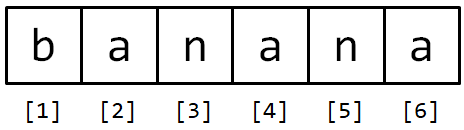
\includegraphics[width=2.61458in,height=\textheight]{images/string-banana.png}

}

\caption{\label{fig-banana-string}바나나 문자열}

\end{figure}%

인덱스로 문자와 연산자를 포함하는 어떤 표현식도 사용 가능지만, 인덱스
값은 정수일 필요는 없다. 정수가 아닌 경우 다음과 같은 결과를 얻게 된다.
문제는 R에서 \texttt{1.5}를 내려서 \texttt{1}로 처리한다는 점이다.
경우에 따라서는 반올림으로 판단해서 \texttt{2}가 될 수도 있어 오해의
소지가 있기 때문에 무조건 정수로 표현한다. \index{인덱스}
\index{예외!자료형 오류} \index{자료형 오류}

\subsection{R}

\begin{Shaded}
\begin{Highlighting}[]
\NormalTok{\#| label: r{-}string{-}integer}
\NormalTok{fruit\_letter[1.5]}
\end{Highlighting}
\end{Shaded}

\subsection{파이썬}

\begin{Shaded}
\begin{Highlighting}[]
\NormalTok{\#| label: py{-}string{-}integer}
\NormalTok{letter = fruit[1.5]}
\NormalTok{\#\textgreater{} TypeError: string indices must be integers}
\end{Highlighting}
\end{Shaded}

\section{\texorpdfstring{\texttt{length()} 함수 사용 문자열 길이
구하기}{length() 함수 사용 문자열 길이 구하기}}\label{r-string-length}

\texttt{length()} 함수는 문자열의 문자 갯수를 반환하는 내장함수다.
\index{length 함수} \index{함수!length}

\subsection{R}

\begin{Shaded}
\begin{Highlighting}[]
\NormalTok{\#| label: r{-}string{-}length}
\NormalTok{fruit \textless{}{-} \textquotesingle{}banana\textquotesingle{}}
\NormalTok{fruit\_letter \textless{}{-} strsplit(fruit, "")[[1]]}

\NormalTok{length(fruit\_letter)}
\end{Highlighting}
\end{Shaded}

\subsection{파이썬}

\begin{Shaded}
\begin{Highlighting}[]
\NormalTok{\#| label: py{-}string{-}length}
\NormalTok{fruit = \textquotesingle{}banana\textquotesingle{}}
\NormalTok{len(fruit)}
\NormalTok{\#\textgreater{} 6}
\end{Highlighting}
\end{Shaded}

문자열의 가장 마지막 문자를 얻기 위해서, 아래와 같이 시도하고 싶을
것이다. \index{예외!인덱스 오류} \index{인덱스 오류}

\subsection{R}

\begin{Shaded}
\begin{Highlighting}[]
\NormalTok{\#| label: r{-}string{-}last}
\NormalTok{len \textless{}{-} length(fruit\_letter)}
\NormalTok{fruit\_letter[len]}
\end{Highlighting}
\end{Shaded}

\subsection{파이썬}

\begin{Shaded}
\begin{Highlighting}[]
\NormalTok{\#| label: py{-}string{-}last}
\NormalTok{length = len(fruit)}
\NormalTok{last = fruit[length]}
\NormalTok{\#\textgreater{} IndexError: string index out of range}
\end{Highlighting}
\end{Shaded}

파이썬에서는 인덱스 오류(IndexError)가 발생하는데 이유는 'banana'에 6번
인덱스 문자가 없기 때문이다. 0에서부터 시작했기 때문에 6개 문자는
0에서부터 5까지 번호가 매겨졌다. 마지막 문자를 얻기 위해서 length에서
1을 빼야 한다. \texttt{fruit{[}-1{]}}은 마지막 문자를,
\texttt{fruit{[}-2{]}}는 끝에서 두 번째 문자를 가리킨다. 하지만, R에서는
사람이 생각하는 방식대로 마지막 문자를 얻는다. \index{인덱스!음수}
\index{음수 인덱스}

\section{루프를 사용한 문자열 순회}\label{r-string-traversal}

\index{순회} \index{루프!순회} \index{for 문} \index{루프!for}
\index{문장!for}

연산의 많은 경우에 문자열을 한 번에 한 문자씩 처리한다. 종종 처음에서
시작해서, 차례로 각 문자를 선택하고, 선택된 문자에 임의 연산을 수행하고,
끝까지 계속한다. 이런 처리 패턴을 \textbf{순회(traversal)}라고 한다.
순회를 작성하는 한 방법이 \texttt{while} 루프다.

\subsection{R}

\begin{Shaded}
\begin{Highlighting}[]
\NormalTok{\#| label: r{-}string{-}traversal}
\NormalTok{index \textless{}{-} 1}

\NormalTok{while(index \textless{}= length(fruit\_letter))\{}
\NormalTok{  letter \textless{}{-} fruit\_letter[index]}
\NormalTok{  print(letter)}
\NormalTok{  index \textless{}{-} index + 1}
\NormalTok{\}}
\end{Highlighting}
\end{Shaded}

\subsection{파이썬}

\begin{Shaded}
\begin{Highlighting}[]
\NormalTok{\#| label: py{-}string{-}traversal}
\NormalTok{index = 0}

\NormalTok{while index \textless{} len(fruit):}
\NormalTok{    letter = fruit[index]}
\NormalTok{    print(letter)}
\NormalTok{    index = index + 1}
\end{Highlighting}
\end{Shaded}

\texttt{while} 루프가 문자열을 순회하여 문자열을 한 줄에 한 글자씩
화면에 출력한다. 루프 조건이
\texttt{index\ \textless{}=\ length(fruit\_letter)}이어서,
\texttt{index}가 문자열 길이와 같을 때, 조건은 거짓이 되고, 루프의 몸통
부문은 실행되지 않는다. R이 접근한 마지막 \texttt{length(fruit\_letter)}
인덱스 문자로, 문자열의 마지막 문자다.

\begin{tcolorbox}[enhanced jigsaw, coltitle=black, breakable, opacityback=0, colback=white, bottomtitle=1mm, titlerule=0mm, toptitle=1mm, title=\textcolor{quarto-callout-warning-color}{\faExclamationTriangle}\hspace{0.5em}{연습문제}, left=2mm, rightrule=.15mm, colframe=quarto-callout-warning-color-frame, bottomrule=.15mm, leftrule=.75mm, toprule=.15mm, arc=.35mm, colbacktitle=quarto-callout-warning-color!10!white, opacitybacktitle=0.6]

문자열의 마지막 문자에서 시작해서, 문자열 처음으로 역진행하면서 한 줄에
한 자씩 화면에 출력하는 \texttt{while} 루프를 작성하세요.

\end{tcolorbox}

순회를 작성하는 또 다른 방법은 \texttt{for} 루프다.

\subsection{R}

\begin{Shaded}
\begin{Highlighting}[]
\NormalTok{\#| label: r{-}string{-}banana{-}for}
\NormalTok{for(char in fruit\_letter) \{}
\NormalTok{  print(char)}
\NormalTok{\}}
\end{Highlighting}
\end{Shaded}

\subsection{파이썬}

\begin{Shaded}
\begin{Highlighting}[]
\NormalTok{\#| label: py{-}string{-}banana{-}for\}}
\NormalTok{for char in fruit:}
\NormalTok{    print(char)}
\end{Highlighting}
\end{Shaded}

루프를 매번 반복할 때, 문자열 다음 문자가 변수 \texttt{char}에 대입된다.
루프는 더 이상 남겨진 문자가 없을 때까지 계속 실행된다.

\section{문자열 슬라이스}\label{r-string-slice}

\index{슬라이스 연산자} \index{연산자!슬라이스} \index{인덱스!슬라이스}
\index{문자열!슬라이스} \index{슬라이스!문자열}

문자열의 일부분을 \textbf{슬라이스(slice)}라고 한다. 문자열 슬라이스를
선택하는 것은 문자를 선택하는 것과 유사하다.

\subsection{R}

\begin{Shaded}
\begin{Highlighting}[]
\NormalTok{\#| label: r{-}string{-}slice\}}
\NormalTok{s \textless{}{-} strsplit(\textquotesingle{}Monty Python\textquotesingle{}, "")[[1]]}
\NormalTok{paste(s[1:5], collapse="")}
\NormalTok{\#\textgreater{} [1] "Monty"}
\NormalTok{paste(s[7:12], collapse="")}
\NormalTok{\#\textgreater{} [1] "Python"}
\end{Highlighting}
\end{Shaded}

\subsection{파이썬}

\begin{Shaded}
\begin{Highlighting}[]
\NormalTok{\#| label: py{-}string{-}slice\}}
\NormalTok{s = \textquotesingle{}Monty Python\textquotesingle{}}
\NormalTok{print(s[0:5])}
\NormalTok{\#\textgreater{} [1] "Monty"}
\NormalTok{print(s[6:13])}
\NormalTok{\#\textgreater{} [1] "Python"}
\end{Highlighting}
\end{Shaded}

\texttt{{[}n:m{]}} 연산자는 \texttt{n}번째 문자부터 \texttt{m}번째
문자까지의 문자열 부분을 반환한다.

파이썬에서 \texttt{fruit{[}:3{]}}와 같이 콜론 앞 첫 인덱스를 생략하면,
문자열 슬라이스는 문자열 처음부터 시작한다. 파이썬에서
\texttt{fruit{[}3:{]}}와 같이 두 번째 인덱스를 생략하면, 문자열
슬라이스는 문자열 끝까지 간다.

이와 동일한 역할을 수행하는 방법은 \texttt{head(fruit\_letter,\ 3)},
\texttt{tail(fruit\_letter,\ 3)}와 같이 \texttt{head()}, \texttt{tail()}
함수를 활용한다.

\subsection{R}

\begin{Shaded}
\begin{Highlighting}[]
\NormalTok{\#| label: r{-}string{-}slice{-}banana}
\NormalTok{fruit \textless{}{-} \textquotesingle{}banana\textquotesingle{}}
\NormalTok{fruit\_letter \textless{}{-} strsplit(fruit, "")[[1]]}

\NormalTok{paste(head(fruit\_letter, 3), collapse="")}
\NormalTok{paste(tail(fruit\_letter, 3), collapse="")}
\end{Highlighting}
\end{Shaded}

\subsection{파이썬}

\begin{Shaded}
\begin{Highlighting}[]
\NormalTok{\#| label: py{-}string{-}slice{-}banana}
\NormalTok{fruit = \textquotesingle{}banana\textquotesingle{}}

\NormalTok{fruit[:3]}
\NormalTok{fruit[3:]}
\end{Highlighting}
\end{Shaded}

만약 첫 번째 인덱스가 두 번째보다 크거나 같은 경우 파이썬에서는 결과가
인용부호로 표현되는 빈 문자열(empty string)이 된다. 하지만, R에서는 해당
인덱스에 해당되는 문자가 추출된다. \index{인용 부호}

\subsection{R}

\begin{Shaded}
\begin{Highlighting}[]
\NormalTok{\#| label: r{-}string{-}slice{-}empty}
\NormalTok{fruit\_letter[3:3]}
\end{Highlighting}
\end{Shaded}

\subsection{파이썬}

\begin{Shaded}
\begin{Highlighting}[]
\NormalTok{\#| label: py{-}string{-}slice{-}empty}
\NormalTok{fruit = \textquotesingle{}banana\textquotesingle{}}
\NormalTok{fruit[3:3]}
\NormalTok{\#\textgreater{} \textquotesingle{}\textquotesingle{}}
\end{Highlighting}
\end{Shaded}

빈 문자열은 어떤 문자도 포함하지 않아서 길이가 0이지만, 이것을 제외하고
다른 문자열과 동일하다. \index{복사!슬라이스} \index{슬라이스!복사}

\begin{tcolorbox}[enhanced jigsaw, coltitle=black, breakable, opacityback=0, colback=white, bottomtitle=1mm, titlerule=0mm, toptitle=1mm, title=\textcolor{quarto-callout-warning-color}{\faExclamationTriangle}\hspace{0.5em}{연습문제 (파이썬)}, left=2mm, rightrule=.15mm, colframe=quarto-callout-warning-color-frame, bottomrule=.15mm, leftrule=.75mm, toprule=.15mm, arc=.35mm, colbacktitle=quarto-callout-warning-color!10!white, opacitybacktitle=0.6]

\texttt{fruit}이 문자열로 주어졌을 때, \texttt{fruit{[}:{]}}의 의미는
무엇인가요?

\end{tcolorbox}

\section{문자열은 불변이다
(파이썬)}\label{uxbb38uxc790uxc5f4uxc740-uxbd88uxbcc0uxc774uxb2e4-uxd30cuxc774uxc36c}

\index{가변성} \index{불변성} \index{문자열!불변성}

문자열 내부에 있는 문자를 변경하려고 대입문 왼쪽편에 \texttt{{[}{]}}
연산자를 사용하고 싶은 유혹이 있을 것이다. 예를 들어 다음과 같다.
\index{자료형 오류} \index{예외!자료형 오류}

\subsection{R}

\begin{Shaded}
\begin{Highlighting}[]
\NormalTok{\#| label: r{-}string{-}immutable}
\NormalTok{greeting \textless{}{-} strsplit(\textquotesingle{}Hello, world!\textquotesingle{}, "")[[1]]}
\NormalTok{greeting[1] \textless{}{-} \textquotesingle{}J\textquotesingle{}}

\NormalTok{paste0(greeting, collapse="")}
\end{Highlighting}
\end{Shaded}

\subsection{파이썬}

\begin{Shaded}
\begin{Highlighting}[]
\NormalTok{\#| label: py{-}string{-}immutable}
\NormalTok{greeting = \textquotesingle{}Hello, world!\textquotesingle{}}
\NormalTok{greeting[0] = \textquotesingle{}J\textquotesingle{}}
\NormalTok{\#\textgreater{} TypeError: \textquotesingle{}str\textquotesingle{} object does not support item assignment}

\NormalTok{greeting = \textquotesingle{}Hello, world!\textquotesingle{}}
\NormalTok{new\_greeting = \textquotesingle{}J\textquotesingle{} + greeting[1:]}
\NormalTok{print(new\_greeting)}
\NormalTok{\#\textgreater{} Jello, world!}
\end{Highlighting}
\end{Shaded}

파이썬에서 ``TypeError: `str' object does not support item assignment''
오류가 발생하는데 파이썬 문자열이 불변(immutable)하기 때문이다. 즉,
파이썬에서 문자열의 특정 문자를 직접 변경하려고 할 때 이 오류가
발생한다. 반면에, R에서는 문자열 자체가 불변 객체로 취급되지 않기 때문에
\texttt{strsplit} 함수를 사용하여 문자열을 문자의 벡터로 변환하면,
벡터의 각 요소는 별도의 문자열로 취급되어 개별적으로 변경할 수 있다. R은
파이썬과 달리 불변 문자열에 대한 제약이 없기 때문에 오류를
발생시키지않는다.

파이썬에서 ``객체(object)''는 문자열이고, 대입하고자 하는 문자는
``항목(item)''이다. 지금으로서 객체는 값과 동일하지만, 나중에 객체
정의를 좀 더 상세화할 것이다. 항목은 순서 값 중의 하나다. 최선의 방법은
원래 문자열을 변형한 새로운 문자열을 생성하는 것이다. \index{객체}
\index{항목 대입} \index{대입!항목} \index{불변성}

새로운 첫 문자에 \texttt{greeting} 문자열 슬라이스를 연결한다. 원래
문자열에는 어떤 영향도 주지 않는 새로운 문자열이 생성되었다.
\index{접합}

\section{루프 사용 문자 계수하기}\label{r-string-count}

\index{계수기} \index{계수와 루프 돌기} \index{루프 돌기와 계수}
\index{루프 돌기!문자열}

다음 프로그램은 문자열에 문자 \texttt{a}가 나타나는 횟수를
계수(counting)한다.

\subsection{R}

\begin{Shaded}
\begin{Highlighting}[]
\NormalTok{\#| label:  r{-}string{-}a{-}count}
\NormalTok{word \textless{}{-} strsplit(\textquotesingle{}banana\textquotesingle{}, "")[[1]]}
\NormalTok{count \textless{}{-} 0}
\NormalTok{for(letter in word) \{}
\NormalTok{  if(letter == \textquotesingle{}a\textquotesingle{})\{}
\NormalTok{    count \textless{}{-} count + 1}
\NormalTok{  \}}
\NormalTok{\}}

\NormalTok{count}
\end{Highlighting}
\end{Shaded}

\subsection{파이썬}

\begin{Shaded}
\begin{Highlighting}[]
\NormalTok{\#| label: py{-}string{-}a{-}count}
\NormalTok{word = \textquotesingle{}banana\textquotesingle{}}
\NormalTok{count = 0}

\NormalTok{for letter in word:}
\NormalTok{    if letter == \textquotesingle{}a\textquotesingle{}:}
\NormalTok{        count = count + 1}

\NormalTok{print(count)}
\end{Highlighting}
\end{Shaded}

상기 프로그램은 \textbf{계수기(counter)}라고 부르는 또 다른 연산 패턴을
보여준다. 변수 count는 0으로 초기화되고, 매번 \texttt{a}를 찾을 때마다
증가한다. 루프를 빠져나갔을 때, \texttt{count}는 결과 값 즉, a가 나타난
총 횟수를 담고 있다.

\begin{tcolorbox}[enhanced jigsaw, coltitle=black, breakable, opacityback=0, colback=white, bottomtitle=1mm, titlerule=0mm, toptitle=1mm, title=\textcolor{quarto-callout-warning-color}{\faExclamationTriangle}\hspace{0.5em}{연습문제}, left=2mm, rightrule=.15mm, colframe=quarto-callout-warning-color-frame, bottomrule=.15mm, leftrule=.75mm, toprule=.15mm, arc=.35mm, colbacktitle=quarto-callout-warning-color!10!white, opacitybacktitle=0.6]

문자열과 문자를 인자(argument)로 받도록 상기 코드를 \texttt{count}라는
함수로 \textbf{캡슐화(encapsulation)}하고 일반화하세요. \index{캡슐화}

\end{tcolorbox}

\section{\texorpdfstring{\texttt{\%in\%}
연산자}{\%in\% 연산자}}\label{r-string-in-operator}

\textbackslash index\{\%in\% 연산자\}
\textbackslash index\{연산자!\%in\%\} \index{부울 연산자}
\index{연산자!부울}

연산자 \texttt{in}은 부울 연산자로 두 개의 문자열을 받아, 첫 번째
문자열이 두 번째 문자열의 일부이면 참(TRUE)을 반환한다.

\subsection{R}

\begin{Shaded}
\begin{Highlighting}[]
\NormalTok{\#| label: r{-}string{-}in{-}op}
\NormalTok{\textquotesingle{}a\textquotesingle{} \%in\% strsplit(\textquotesingle{}banana\textquotesingle{}, "")[[1]]}
\NormalTok{\textquotesingle{}seed\textquotesingle{} \%in\% strsplit(\textquotesingle{}banana\textquotesingle{}, "")[[1]]}
\end{Highlighting}
\end{Shaded}

\subsection{파이썬}

\begin{Shaded}
\begin{Highlighting}[]
\NormalTok{\#| label: py{-}string{-}in{-}op}
\NormalTok{\textquotesingle{}a\textquotesingle{} in \textquotesingle{}banana\textquotesingle{}}
\NormalTok{\#\textgreater{} True}
\NormalTok{\textquotesingle{}seed\textquotesingle{} in \textquotesingle{}banana\textquotesingle{}}
\NormalTok{\#\textgreater{} False}
\end{Highlighting}
\end{Shaded}

\section{문자열 비교}\label{r-string-comparison-operator}

\index{문자열!비교} \index{비교!문자열}

비교 연산자도 문자열에서 동작한다. 두 문자열이 같은지를 살펴보자.

\subsection{R}

\begin{Shaded}
\begin{Highlighting}[]
\NormalTok{\#| label: r{-}string{-}comparison}
\NormalTok{word \textless{}{-} \textquotesingle{}banana\textquotesingle{}}

\NormalTok{if(word == \textquotesingle{}banana\textquotesingle{}) \{}
\NormalTok{  print(\textquotesingle{}All right, bananas.\textquotesingle{})}
\NormalTok{\}}
\end{Highlighting}
\end{Shaded}

\subsection{파이썬}

\begin{Shaded}
\begin{Highlighting}[]
\NormalTok{\#| label: py{-}string{-}comparison}
\NormalTok{word = \textquotesingle{}banana\textquotesingle{}}

\NormalTok{if word == \textquotesingle{}banana\textquotesingle{}:}
\NormalTok{    print(\textquotesingle{}All right, bananas.\textquotesingle{})}
\end{Highlighting}
\end{Shaded}

다른 비교 연산자는 단어를 알파벳 순서로 정렬하는 데 유용하다.

\subsection{R}

\begin{Shaded}
\begin{Highlighting}[]
\NormalTok{\#| label: r{-}string{-}pineapple}
\NormalTok{word \textless{}{-} \textquotesingle{}Pineapple\textquotesingle{}}

\NormalTok{if(word \textless{} \textquotesingle{}banana\textquotesingle{}) \{}
\NormalTok{  message(\textquotesingle{}Your word \textquotesingle{},  word, \textquotesingle{} comes before banana.\textquotesingle{})}
\NormalTok{\} else if (word \textgreater{} \textquotesingle{}banana\textquotesingle{}) \{}
\NormalTok{  message(\textquotesingle{}Your word \textquotesingle{}, word, \textquotesingle{} comes after banana.\textquotesingle{})}
\NormalTok{\} else \{}
\NormalTok{  message(\textquotesingle{}All right, bananas.\textquotesingle{})}
\NormalTok{\}}
\end{Highlighting}
\end{Shaded}

\subsection{파이썬}

\begin{Shaded}
\begin{Highlighting}[]
\NormalTok{\#| label: py{-}string{-}pineapple}
\NormalTok{word = \textquotesingle{}Pineapple\textquotesingle{}}

\NormalTok{if word \textless{} \textquotesingle{}banana\textquotesingle{}:}
\NormalTok{    print(\textquotesingle{}Your word, \textquotesingle{} + word + \textquotesingle{}, comes before banana.\textquotesingle{})}
\NormalTok{elif word \textgreater{} \textquotesingle{}banana\textquotesingle{}:}
\NormalTok{    print(\textquotesingle{}Your word, \textquotesingle{} + word + \textquotesingle{}, comes after banana.\textquotesingle{})}
\NormalTok{else:}
\NormalTok{    print(\textquotesingle{}All right, bananas.\textquotesingle{})}
\end{Highlighting}
\end{Shaded}

R과 파이썬 같은 프로그래밍 언어는 사람과 동일한 방식으로 대문자와
소문자를 다루지 않는다. 모든 대문자는 소문자 앞에 온다. 프로그래밍
언어에서 대문자와 소문자를 다루는 방식은 ASCII 코드 값을 기반으로 한다.
ASCII 코드에서 대문자(A-Z)는 65부터 90까지의 값을, 소문자(a-z)는 97부터
122까지의 값을 갖기 때문에 대문자가 숫자적으로 소문자보다 먼저 나오기
때문에 문자열을 정렬하거나 비교할 때, 대문자가 소문자 앞에 위치하게
된다.

\begin{Shaded}
\begin{Highlighting}[]
\ExtensionTok{Your}\NormalTok{ word, Pineapple, comes before banana.}
\end{Highlighting}
\end{Shaded}

이러한 문제를 다루는 일반적인 방식은 비교 연산을 수행하기 전에 문자열을
표준 포맷으로 예를 들어 모두 소문자로 변환하는 것이다. 경우에 따라서
``Pineapple''로 무장한 사람들로부터 여러분을 보호해야 하는 것도
명심한다.

\section{문자열 함수}\label{r-string-method}

R은 객체지향언어 특성을 갖고 있지만 함수형 프로그래밍 언어 특성도 갖고
있다. 문자열을 R 객체(objects)로 객체를 데이터(실제 문자열 자체)와
메서드(methods)를 담고 있는 것으로 바라볼 수도 있다. 메서드는 객체에
내장되고 어떤 객체의 인스턴스(instance)에도 사용되는 사실상 함수다.
\index{메서드} \index{문자열!메서드} \index{점 표기법} \index{괄호!빈}
\index{호출}

\begin{tcolorbox}[enhanced jigsaw, coltitle=black, breakable, opacityback=0, colback=white, bottomtitle=1mm, titlerule=0mm, toptitle=1mm, title=\textcolor{quarto-callout-note-color}{\faInfo}\hspace{0.5em}{파이썬 \texttt{dir} 함수}, left=2mm, rightrule=.15mm, colframe=quarto-callout-note-color-frame, bottomrule=.15mm, leftrule=.75mm, toprule=.15mm, arc=.35mm, colbacktitle=quarto-callout-note-color!10!white, opacitybacktitle=0.6]

객체에 대해 이용 가능한 메서드를 보여주는 \texttt{dir} 함수가 파이썬에
있다. \texttt{type} 함수는 객체의 자료형(type)을 보여주고,
\texttt{dir}은 객체에 사용될 수 있는 메서드를 보여준다.

\begin{Shaded}
\begin{Highlighting}[]
\NormalTok{\#| label: py{-}string{-}dir}
\NormalTok{\#| }
\NormalTok{stuff = \textquotesingle{}Hello world\textquotesingle{}}
\NormalTok{type(stuff)}
\NormalTok{\#\textgreater{} \textless{}type \textquotesingle{}str\textquotesingle{}\textgreater{}}
\NormalTok{methods = [method for method in dir(stuff) if not method.startswith(\textquotesingle{}\_\_\textquotesingle{}) and not method.endswith(\textquotesingle{}\_\_\textquotesingle{})]}
\NormalTok{methods}
\NormalTok{\#\textgreater{} [\textquotesingle{}capitalize\textquotesingle{}, \textquotesingle{}casefold\textquotesingle{}, \textquotesingle{}center\textquotesingle{}, \textquotesingle{}count\textquotesingle{}, \textquotesingle{}encode\textquotesingle{}, \textquotesingle{}endswith\textquotesingle{}, \textquotesingle{}expandtabs\textquotesingle{}, \textquotesingle{}find\textquotesingle{}, \textquotesingle{}format\textquotesingle{}, \textquotesingle{}format\_map\textquotesingle{}, \textquotesingle{}index\textquotesingle{}, \textquotesingle{}isalnum\textquotesingle{}, \textquotesingle{}isalpha\textquotesingle{}, \textquotesingle{}isascii\textquotesingle{}, \textquotesingle{}isdecimal\textquotesingle{}, \textquotesingle{}isdigit\textquotesingle{}, \textquotesingle{}isidentifier\textquotesingle{}, \textquotesingle{}islower\textquotesingle{}, \textquotesingle{}isnumeric\textquotesingle{}, \textquotesingle{}isprintable\textquotesingle{}, \textquotesingle{}isspace\textquotesingle{}, \textquotesingle{}istitle\textquotesingle{}, \textquotesingle{}isupper\textquotesingle{}, \textquotesingle{}join\textquotesingle{}, \textquotesingle{}ljust\textquotesingle{}, \textquotesingle{}lower\textquotesingle{}, \textquotesingle{}lstrip\textquotesingle{}, \textquotesingle{}maketrans\textquotesingle{}, \textquotesingle{}partition\textquotesingle{}, \textquotesingle{}removeprefix\textquotesingle{}, \textquotesingle{}removesuffix\textquotesingle{}, \textquotesingle{}replace\textquotesingle{}, \textquotesingle{}rfind\textquotesingle{}, \textquotesingle{}rindex\textquotesingle{}, \textquotesingle{}rjust\textquotesingle{}, \textquotesingle{}rpartition\textquotesingle{}, \textquotesingle{}rsplit\textquotesingle{}, \textquotesingle{}rstrip\textquotesingle{}, \textquotesingle{}split\textquotesingle{}, \textquotesingle{}splitlines\textquotesingle{}, \textquotesingle{}startswith\textquotesingle{}, \textquotesingle{}strip\textquotesingle{}, \textquotesingle{}swapcase\textquotesingle{}, \textquotesingle{}title\textquotesingle{}, \textquotesingle{}translate\textquotesingle{}, \textquotesingle{}upper\textquotesingle{}, \textquotesingle{}zfill\textquotesingle{}]}
\end{Highlighting}
\end{Shaded}

\texttt{dir} 함수가 메서드 목록을 보여주고, 메서드에 대한 간단한 문서
정보는 \texttt{help}를 사용할 수 있지만, 문자열 메서드에 대한 좀 더 좋은
문서 정보는 \url{https://docs.python.org/3/library/string.html}에서 찾을
수 있다.

인자를 받고 값을 반환한다는 점에서 메서드(method)를 호출하는 것은 함수를
호출하는 것과 유사하지만, 구문은 다르다. 구분자로 점을 사용해서 변수명에
메서드명을 붙여 메서드를 호출한다.

예를 들어, \texttt{upper} 메서드는 문자열을 받아 모두 대문자로 변환된
새로운 문자열을 반환한다. 함수 구문 \texttt{upper(word)} 대신에,
\texttt{word.upper()} 메서드 구문을 사용한다.

\end{tcolorbox}

하지만, 함수형 프로그래밍 패러다임으로 문자열을 객체로 두고 함수를
적용시켜 다양한 작업을 하는 것이 일반적이다. \texttt{tidyverse} 패키지를
설치하게 되면 \texttt{stringr} 패키지가 구성요소로 포함되어 있다.
\texttt{str\_}로 시작되는 다양한 함수가 지원된다. \index{계수 메서드}
\index{메서드!계수}

예를 들어, \texttt{stringr} 패키지 \texttt{str\_to\_upper()} 함수는
문자열을 받아 모두 대문자로 변환된 새로운 문자열을 반환한다.

\subsection{R}

\begin{Shaded}
\begin{Highlighting}[]
\NormalTok{\#| label: r{-}string{-}upper}
\NormalTok{library(stringr)}

\NormalTok{word \textless{}{-} \textquotesingle{}banana\textquotesingle{}}
\NormalTok{new\_word \textless{}{-} stringr::str\_to\_upper(word)}
\NormalTok{new\_word}
\NormalTok{\#\textgreater{} [1] "BANANA"}
\end{Highlighting}
\end{Shaded}

\subsection{파이썬}

\begin{Shaded}
\begin{Highlighting}[]
\NormalTok{\#| label: r{-}string{-}upper}
\NormalTok{word = \textquotesingle{}banana\textquotesingle{}}
\NormalTok{new\_word = word.upper()}
\NormalTok{print(new\_word)}
\NormalTok{\#\textgreater{} BANANA}
\end{Highlighting}
\end{Shaded}

동일한 작업을 함수형 패러다임으로 \texttt{str\_to\_upper(word)}와 같이
표현하는 데 반해, 객체지향으로 구현하면 파이썬 같은 경우
\texttt{word.upper()} 메서드 구문이 사용된다.

예를 들어, 문자열 안에 문자열의 위치를 찾는 \texttt{str\_locate()},
\texttt{str\_locate\_all()}이라는 문자열 함수가 있다.
\texttt{str\_locate()}는 매칭되는 첫 번째만 반환하는 반면에
\texttt{str\_locate\_all()}은 매칭되는 전부를 반환하는 차이가 있다.

\subsection{R}

\begin{Shaded}
\begin{Highlighting}[]
\NormalTok{\#| label: r{-}string{-}locate}
\NormalTok{str\_locate(word, \textquotesingle{}a\textquotesingle{})}
\NormalTok{\#\textgreater{}      start end}
\NormalTok{\#\textgreater{} [1,]     2   2}
\end{Highlighting}
\end{Shaded}

\subsection{파이썬}

\begin{Shaded}
\begin{Highlighting}[]
\NormalTok{\#| label: py{-}string{-}locate}
\NormalTok{word = \textquotesingle{}banana\textquotesingle{}}
\NormalTok{index = word.find(\textquotesingle{}a\textquotesingle{})}
\NormalTok{print(index)}
\NormalTok{\#\textgreater{} 1}
\end{Highlighting}
\end{Shaded}

상기 예제에서, word 문자열에 \texttt{str\_locate\_all()} 함수를 호출하여
매개 변수로 찾고자 하는 문자를 넘긴다.

\texttt{str\_locate\_all()} 함수로 문자뿐만 아니라 부속
문자열(substring)도 찾을 수 있다.

\subsection{R}

\begin{Shaded}
\begin{Highlighting}[]
\NormalTok{\#| label: r{-}string{-}locate{-}substring}
\NormalTok{str\_locate\_all(word, \textquotesingle{}na\textquotesingle{})[[1]]}
\NormalTok{\#\textgreater{}      start end}
\NormalTok{\#\textgreater{} [1,]     3   4}
\NormalTok{\#\textgreater{} [2,]     5   6}
\end{Highlighting}
\end{Shaded}

\subsection{파이썬}

\begin{Shaded}
\begin{Highlighting}[]
\NormalTok{\#| label: py{-}string{-}locate{-}substring}
\NormalTok{word.find(\textquotesingle{}na\textquotesingle{})}
\NormalTok{\#\textgreater{} 2}
\NormalTok{word.find(\textquotesingle{}na\textquotesingle{}, 3)}
\NormalTok{\#\textgreater{} 4}
\end{Highlighting}
\end{Shaded}

한 가지 자주 있는 작업은 \texttt{str\_trim()} 함수를 사용해서 문자열
시작과 끝의 공백(공백 여러 개, 탭, 새줄)을 제거하는 것이다.

\subsection{R}

\begin{Shaded}
\begin{Highlighting}[]
\NormalTok{\#| label: r{-}string{-}strip}
\NormalTok{line \textless{}{-} \textquotesingle{}     Here we go \textquotesingle{}}
\NormalTok{str\_trim(line)}
\NormalTok{\#\textgreater{} [1] "Here we go"}
\end{Highlighting}
\end{Shaded}

\subsection{파이썬}

\begin{Shaded}
\begin{Highlighting}[]
\NormalTok{\#| label: py{-}string{-}strip}
\NormalTok{line = \textquotesingle{}     Here we go \textquotesingle{}}
\NormalTok{line.strip()}
\NormalTok{\#\textgreater{} \textquotesingle{}Here we go\textquotesingle{}}
\end{Highlighting}
\end{Shaded}

\texttt{str\_detect()} 함수와 나중에 다룰 정규표현식을 섞어 표현하게
되면 참, 거짓 같은 부울 값(boolean value)을 반환한다.
\texttt{\textquotesingle{}\^{}Please\textquotesingle{}}에서
\texttt{\^{}}은 문자열 시작을 지정한다.

\subsection{R}

\begin{Shaded}
\begin{Highlighting}[]
\NormalTok{\#| label: r{-}string{-}startwith}
\NormalTok{line \textless{}{-} \textquotesingle{}좋은 하루되세요!\textquotesingle{}}
\NormalTok{str\_detect(line, \textquotesingle{}\^{}좋은\textquotesingle{})}
\NormalTok{\#\textgreater{} [1] TRUE}
\end{Highlighting}
\end{Shaded}

\subsection{파이썬}

\begin{Shaded}
\begin{Highlighting}[]
\NormalTok{\#| label: py{-}string{-}startwith}
\NormalTok{line = \textquotesingle{}좋은 하루되세요!\textquotesingle{}}
\NormalTok{line.startswith(\textquotesingle{}좋은\textquotesingle{})}
\NormalTok{\#\textgreater{} True}
\NormalTok{line.startswith(\textquotesingle{}조은\textquotesingle{})}
\NormalTok{\#\textgreater{} False}
\end{Highlighting}
\end{Shaded}

대소문자를 구별하는 것을 요구하기 때문에 \texttt{str\_to\_lower()}
함수를 사용해서 검증을 수행하기 전에, 한 줄을 입력받아 모두 소문자로
변환하는 것이 필요하다.

\subsection{R}

\begin{Shaded}
\begin{Highlighting}[]
\NormalTok{\#| label: r{-}string{-}startwith{-}to{-}lower}
\NormalTok{line \textless{}{-} \textquotesingle{}Please have a nice day\textquotesingle{}}
\NormalTok{str\_detect(line, \textquotesingle{}\^{}p\textquotesingle{})}

\NormalTok{str\_to\_lower(line)}

\NormalTok{str\_detect(str\_to\_lower(line), \textquotesingle{}\^{}p\textquotesingle{})}
\end{Highlighting}
\end{Shaded}

\subsection{파이썬}

\begin{Shaded}
\begin{Highlighting}[]
\NormalTok{\#| label: py{-}string{-}startwith{-}to{-}lower}
\NormalTok{line = \textquotesingle{}Please have a nice day\textquotesingle{}}
\NormalTok{line.startswith(\textquotesingle{}p\textquotesingle{})}
\NormalTok{\#\textgreater{} False}
\NormalTok{line.lower()}
\NormalTok{\#\textgreater{} \textquotesingle{}please have a nice day\textquotesingle{}}
\NormalTok{line.lower().startswith(\textquotesingle{}p\textquotesingle{})}
\NormalTok{\#\textgreater{} True}
\end{Highlighting}
\end{Shaded}

마지막 예제에서 문자열이 문자 ``p''로 시작하는지를 검증하기 위해서,
\texttt{str\_to\_lower()} 함수를 호출하고 나서 바로
\texttt{str\_detect()} 함수를 사용한다. 주의 깊게 순서만 다룬다면, 한
줄에 다수 함수를 괄호에 넣어 호출할 수 있다.

\begin{tcolorbox}[enhanced jigsaw, coltitle=black, breakable, opacityback=0, colback=white, bottomtitle=1mm, titlerule=0mm, toptitle=1mm, title=\textcolor{quarto-callout-warning-color}{\faExclamationTriangle}\hspace{0.5em}{연습문제}, left=2mm, rightrule=.15mm, colframe=quarto-callout-warning-color-frame, bottomrule=.15mm, leftrule=.75mm, toprule=.15mm, arc=.35mm, colbacktitle=quarto-callout-warning-color!10!white, opacitybacktitle=0.6]

앞선 예제와 유사한 함수인 \texttt{str\_count()}로 불리는 문자열 메서드가
\texttt{stringr} 패키지 내부에 있다. \texttt{?\ str\_count()} 도움말로
\texttt{str\_count()} 함수에 대한 문서를 읽고, 문자열 'banana'의 문자가
몇 개인지 계수하는 메서드 호출 프로그램을 작성하세요.

\end{tcolorbox}

\section{문자열 파싱}\label{r-string-parsing}

종종, 문자열을 들여다보고 특정 부속 문자열(substring)을 찾고 싶다. 예를
들어, 아래와 같은 형식으로 작성된 일련의 라인이 주어졌다고 가정하면,

\begin{quote}
\texttt{From\ stephen.marquard@}\textbf{uct.ac.za}\texttt{Sat\ Jan\ \ 5\ 09:14:16\ 2008}
\end{quote}

각 라인마다 뒤쪽 전자우편 주소(즉, uct.ac.za)만 뽑아내고 싶을 것이다.
\texttt{str\_locate()} 함수와 문자열 슬라이싱(string sliceing)을
사용해서 작업을 수행할 수 있다.

우선, 문자열에서 골뱅이(\texttt{@}, at-sign) 기호의 위치를 찾는다.
그리고, 골뱅이 기호 뒤 첫 공백 위치를 찾는다. 그리고 나서, 찾고자 하는
부속 문자열을 뽑아내기 위해서 문자열 슬라이싱을 사용한다.

\subsection{R}

\begin{Shaded}
\begin{Highlighting}[]
\NormalTok{\#| label: r{-}string{-}email{-}parsing}
\NormalTok{data \textless{}{-} \textquotesingle{}From stephen.marquard@uct.ac.za Sat Jan 5 09:14:16 2008\textquotesingle{}}
\NormalTok{atpos \textless{}{-} str\_locate(data, \textquotesingle{}@\textquotesingle{})}
\NormalTok{atpos[1,1]}
\NormalTok{\#\textgreater{} start }
\NormalTok{\#\textgreater{}    5 }
\NormalTok{sppos \textless{}{-} str\_locate\_all(data, \textquotesingle{} \textquotesingle{})[[1]]}
\NormalTok{sppos}
\NormalTok{\#\textgreater{}      start end}
\NormalTok{\#\textgreater{} [1,]     5   5}
\NormalTok{\#\textgreater{} [2,]    32  32}
\NormalTok{\#\textgreater{} [3,]    36  36}
\NormalTok{\#\textgreater{} [4,]    40  40}
\NormalTok{\#\textgreater{} [5,]    42  42}
\NormalTok{\#\textgreater{} [6,]    51  51}
\NormalTok{str\_sub(data, start = atpos[1,1] + 1, end = sppos[2,2] {-} 1)}
\NormalTok{\#\textgreater{} [1] "uct.ac.za"}
\end{Highlighting}
\end{Shaded}

\subsection{파이썬}

\begin{Shaded}
\begin{Highlighting}[]
\NormalTok{\#| label: py{-}string{-}email{-}parsing}
\NormalTok{data = \textquotesingle{}From stephen.marquard@uct.ac.za Sat Jan 5 09:14:16 2008\textquotesingle{}}
\NormalTok{atpos = data.find(\textquotesingle{}@\textquotesingle{})}
\NormalTok{print(atpos)}
\NormalTok{\#\textgreater{} 21}
\NormalTok{sppos = data.find(\textquotesingle{} \textquotesingle{},atpos)}
\NormalTok{print(sppos)}
\NormalTok{\#\textgreater{} 31}
\NormalTok{host = data[atpos+1:sppos]}
\NormalTok{print(host)}
\NormalTok{\#\textgreater{} uct.ac.za}
\end{Highlighting}
\end{Shaded}

\texttt{str\_locate()} 함수를 사용해서 찾고자 하는 문자열의 시작 위치를
명세한다. 문자열 슬라이싱(slicing)할 때, 골뱅이 기호 뒤부터 빈 공백을
포함하지 않는 위치까지 문자열을 뽑아낸다.

\section{서식 연산자}\label{r-string-format}

\index{서식 연산자} \index{연산자!서식}

\textbf{서식 연산자(format operator)} Base R의 \texttt{sprintf()} 함수에
C언어 스타일로 \texttt{\%}를 사용하기도 하지만
\href{https://cran.r-project.org/web/packages/glue/index.html}{glue:
Interpreted String Literals} 패키지도 최근에 많이 사용된다.
\texttt{glue} 패키지 \texttt{\{\}}는 문자열 일부를 변수에 저장된 값으로
바꿔 문자열을 구성한다. 정수에 서식 연산자가 적용될 때, \{\}는 나머지
연산자가 된다. 하지만 첫 피연산자가 문자열이면, \{\}은 서식 연산자가
된다. 동일한 기능을 \texttt{stringr} 패키지 \texttt{str\_glue()} 함수로
수행할 수 있다. \index{서식 문자열}

첫 피연산자는 서식 문자열(format string)로 두 번째 피연산자가 어떤
형식으로 표현되는지를 명세하는 하나 혹은 그 이상의 서식 순서(format
sequence)를 담고 있다. 결과값은 문자열이다. \index{서식 순서}

예를 들어, 형식 순서 '\%d'의 의미는 두 번째 피연산자가 정수 형식으로
표현됨을 뜻한다. (d는 ``decimal''을 나타낸다.)

\subsection{R}

\begin{Shaded}
\begin{Highlighting}[]
\NormalTok{\#| label: r{-}string{-}format}
\NormalTok{camels \textless{}{-} 42}
\NormalTok{sprintf(\textquotesingle{}\%d\textquotesingle{}, camels)}
\NormalTok{\#\textgreater{} [1] "42"}
\NormalTok{str\_glue("\{camels\}")}
\NormalTok{\#\textgreater{} 42}
\end{Highlighting}
\end{Shaded}

\subsection{파이썬}

\begin{Shaded}
\begin{Highlighting}[]
\NormalTok{\#| label: py{-}string{-}format}
\NormalTok{camels = 42}
\NormalTok{\textquotesingle{}\%d\textquotesingle{} \% camels}
\NormalTok{\#\textgreater{} \textquotesingle{}42\textquotesingle{}}
\end{Highlighting}
\end{Shaded}

결과는 문자열 '42'로 정수 42와 혼동하면 안 된다.

서식 순서는 문자열 어디에도 나타날 수 있어서 문장 중간에 값을
임베드(embed)할 수 있다.

\subsection{R}

\begin{Shaded}
\begin{Highlighting}[]
\NormalTok{\#| label: r{-}string{-}format{-}camels}
\NormalTok{camels \textless{}{-} 42}
\NormalTok{sprintf(\textquotesingle{}I have spotted \%d camels.\textquotesingle{}, camels)}
\NormalTok{\#\textgreater{} [1] "I have spotted 42 camels."}
\NormalTok{str\_glue(\textquotesingle{}I have spotted \{camels\} camels.\textquotesingle{})}
\NormalTok{\#\textgreater{} I have spotted 42 camels.}
\end{Highlighting}
\end{Shaded}

\subsection{파이썬}

\begin{Shaded}
\begin{Highlighting}[]
\NormalTok{\#| label: py{-}string{-}format{-}camels}
\NormalTok{camels = 42}
\NormalTok{\textquotesingle{}I have spotted \%d camels.\textquotesingle{} \% camels}
\NormalTok{\#\textgreater{} \textquotesingle{}I have spotted 42 camels.\textquotesingle{}}
\end{Highlighting}
\end{Shaded}

만약 문자열 서식 순서가 하나 이상이라면, 두 번째 인자는 튜플(tuple)이
된다. 서식 순서 각각은 순서대로 튜플 요소와 매칭된다.

다음 예제는 정수 형식을 표현하기 위해서 `\%d', 부동 소수점 형식을
표현하기 위해서 `\%g', 문자열 형식을 표현하기 위해서 `\%s'을 사용한
사례다. 여기서 왜 부동 소수점 형식이'\%f' 대신에 '\%g'인지는 질문하지
말아주세요. \index{예외!자료형 오류} \index{자료형 오류}

\subsection{R}

\begin{Shaded}
\begin{Highlighting}[]
\NormalTok{\#| label: r{-}string{-}matching}
\NormalTok{sprintf(\textquotesingle{}In \%d years I have spotted \%g \%s\textquotesingle{}, 3, 0.1, \textquotesingle{}camels\textquotesingle{})}
\NormalTok{\#\textgreater{} [1] "In 3 years I have spotted 0.1 camels"}

\NormalTok{str\_glue(\textquotesingle{}In \{3\} years I have spotted \{0.1\} \{"camels"\}\textquotesingle{})}
\NormalTok{\#\textgreater{} In 3 years I have spotted 0.1 camels}
\end{Highlighting}
\end{Shaded}

\subsection{파이썬}

\begin{Shaded}
\begin{Highlighting}[]
\NormalTok{\#| label: py{-}string{-}matching}
\NormalTok{\# \textasciigrave{}format\textasciigrave{} 메서드}
\NormalTok{result = \textquotesingle{}In \{\} years I have spotted \{\} \{\}\textquotesingle{}.format(3, 0.1, \textquotesingle{}camels\textquotesingle{})}
\NormalTok{print(result)}
\NormalTok{\#\textgreater{} In 3 years I have spotted 0.1 camels}

\NormalTok{\# \textasciigrave{}f{-}string\textasciigrave{}}
\NormalTok{years = 3}
\NormalTok{camels = 0.1}
\NormalTok{result = f\textquotesingle{}In \{years\} years I have spotted \{camels\} \{"camels"\}\textquotesingle{}}
\NormalTok{print(result)}
\NormalTok{\#\textgreater{} In 3 years I have spotted 0.1 camels}
\end{Highlighting}
\end{Shaded}

문자열 서식 순서와 갯수는 일치해야 하고, 요소의 자료형(type)도 서식
순서와 일치해야 한다.

\subsection{R}

\begin{Shaded}
\begin{Highlighting}[]
\NormalTok{\#| label: r{-}string{-}type{-}error}
\NormalTok{sprintf(\textquotesingle{}\%d \%d \%d\textquotesingle{}, 1, 2)}
\NormalTok{\#\textgreater{} sprintf("\%d \%d \%d", 1, 2)에서 다음과 같은 에러가 발생했습니다:인자들의 수가 너무 적습니다}
\NormalTok{sprintf(\textquotesingle{}\%d\textquotesingle{}, \textquotesingle{}dollars\textquotesingle{})}
\NormalTok{\#\textgreater{} sprintf("\%d", "dollars")에서 다음과 같은 에러가 발생했습니다: \textquotesingle{}\%d\textquotesingle{}는 유효하지 않은 포맷입니다; 문자형 객체들에는 포맷 \%s를 사용해주세요}
\end{Highlighting}
\end{Shaded}

\subsection{파이썬}

\begin{Shaded}
\begin{Highlighting}[]
\NormalTok{\#| label: py{-}string{-}type{-}error}
\NormalTok{\textquotesingle{}\%d \%d \%d\textquotesingle{} \% (1, 2)}
\NormalTok{\#\textgreater{} TypeError: not enough arguments for format string}
\NormalTok{\textquotesingle{}\%d\textquotesingle{} \% \textquotesingle{}dollars\textquotesingle{}}
\NormalTok{\#\textgreater{} TypeError: \%d format: a number is required, not str}
\end{Highlighting}
\end{Shaded}

상기 첫 예제는 충분한 요소 개수가 되지 않고, 두 번째 예제는 자료형이
맞지 않는다. 서식 연산자는 강력하지만, 사용하기가 까다로운 점이 있으니,
\texttt{str\_glue}를 사용하는 것도 권장된다.

\section{디버깅}\label{r-string-debug}

\index{디버깅}

프로그램을 작성하면서 배양해야 하는 기술은 항상 자신에게 질문을 하는
것이다. ``여기서 무엇이 잘못될 수 있을까?'' 혹은 ``내가 작성한 완벽한
프로그램을 망가뜨리기 위해 사용자는 무슨 엄청난 일을 할 것인가?''

예를 들어 앞장의 반복 while 루프를 시연하기 위해 사용한 프로그램을
살펴봅시다.

\subsection{R}

\begin{Shaded}
\begin{Highlighting}[]
\NormalTok{\#| label: r{-}string{-}debug}
\NormalTok{while(TRUE) \{}
\NormalTok{  line \textless{}{-} readline(prompt = \textquotesingle{}\textgreater{} \textquotesingle{})}
\NormalTok{  if(substr(line,1,1) == "\#") \{}
\NormalTok{    next}
\NormalTok{  \}}
\NormalTok{  if(line == \textquotesingle{}done\textquotesingle{}) \{}
\NormalTok{    break}
\NormalTok{  \}}
\NormalTok{  print(line)}
\NormalTok{\}}
\end{Highlighting}
\end{Shaded}

\subsection{파이썬}

\begin{Shaded}
\begin{Highlighting}[]
\NormalTok{\#| label: py{-}string{-}debug}
\NormalTok{while True:}
\NormalTok{    line = input(\textquotesingle{}\textgreater{} \textquotesingle{})}
\NormalTok{    if line[0] == \textquotesingle{}\#\textquotesingle{}:}
\NormalTok{        continue}
\NormalTok{    if line == \textquotesingle{}done\textquotesingle{}:}
\NormalTok{        break}
\NormalTok{    print(line)}
\NormalTok{print(\textquotesingle{}Done!\textquotesingle{})}
\end{Highlighting}
\end{Shaded}

사용자가 입력값으로 빈 공백 줄을 입력하게 될 때 무엇이 발생하는지
살펴봅시다.

\begin{Shaded}
\begin{Highlighting}[]
\OperatorTok{\textgreater{}}\NormalTok{ hello }\ExtensionTok{there}
\ExtensionTok{[1]}\NormalTok{ hello there}
\OperatorTok{\textgreater{}} \CommentTok{\# don\textquotesingle{}t print this}
\OperatorTok{\textgreater{}}\NormalTok{ print }\ExtensionTok{this!}
\ExtensionTok{[2]}\NormalTok{ print this!}
\OperatorTok{\textgreater{}} 
\ExtensionTok{[1]} \StringTok{""}
\OperatorTok{\textgreater{}}\NormalTok{ done}
\end{Highlighting}
\end{Shaded}

빈 공백 줄이 입력될 때까지 코드는 잘 작동한다. 그리고 나서, 파이썬의
경우 0번째 문자가 없어서 트레이스백(traceback)이 발생한다. R의 경우 정상
실행되지만 원하는 바는 아니다. 입력 줄이 비어있을 때, 코드 3번째 줄을
``안전''하게 만드는 두 가지 방법이 있다.

하나는 빈 문자열이면 거짓(FALSE)을 반환하도록 \texttt{str\_detect()}
함수를 사용하는 것이다.

\subsection*{R}\label{r-27}
\addcontentsline{toc}{subsection}{R}

\texttt{if(str\_detect(line,\ \textquotesingle{}\^{}\#\textquotesingle{}))}

\subsection*{파이썬}\label{uxd30cuxc774uxc36c-27}
\addcontentsline{toc}{subsection}{파이썬}

\texttt{if\ line.startswith(\textquotesingle{}\#\textquotesingle{})\ :}

\textbf{가디언 패턴(guardian pattern)}을 사용한 \texttt{if}문으로
문자열에 적어도 하나의 문자가 있는 경우만 두 번째 논리 표현식이
평가되도록 코드를 작성한다. \index{가디언 패턴} \index{패턴!가디언}

\subsection*{R}\label{r-28}
\addcontentsline{toc}{subsection}{R}

\texttt{if(str\_length(line)\ \textgreater{}\ 0\ \&\ str\_detect(line,\ \textquotesingle{}\^{}\#\textquotesingle{}))}

\subsection*{파이썬}\label{uxd30cuxc774uxc36c-28}
\addcontentsline{toc}{subsection}{파이썬}

\texttt{if\ len(line)\ \textgreater{}\ 0\ and\ line{[}0{]}\ ==\ \textquotesingle{}\#\textquotesingle{}\ :}

\section{용어 정의}\label{r-string-terminology}

\begin{itemize}
\tightlist
\item
  \textbf{계수기(counter)}: 무언가를 계수하기 위해서 사용되는 변수로
  일반적으로 0으로 초기화하고 나서 증가한다. \index{계수기}
\item
  \textbf{빈 문자열(empty string)}: 두 인용부호로 표현되고, 어떤 문자도
  없고 길이가 0인 문자열. \index{빈 문자열}
\item
  \textbf{서식 연산자(format operator)}: 서식 문자열과 튜플을 받아, 서식
  문자열에 지정된 서식으로 튜플 요소를 포함하는 문자열을 생성하는
  연산자. \index{서식 연산자} \index{연산자!서식}
\item
  \textbf{서식 순서(format sequence)}: d처럼 어떤 값의 서식으로
  표현되어야 하는지를 명세하는 ``서식 문자열'' 문자 순서.
  \index{서식 순서}
\item
  \textbf{서식 문자열(format string)}: 서식 순서를 포함하는 서식
  연산자와 함께 사용되는 문자열. \index{서식 문자열}
\item
  \textbf{플래그(flag)}: 조건이 참인지를 표기하기 위해 사용하는 불
  변수(boolean variable) \index{플래그}
\item
  \textbf{호출(invocation)}: 메서드를 호출하는 명령문. \index{호출}
\item
  \textbf{불변(immutable)}: 순서의 항목에 대입할 수 없는 특성.
  \index{불변}
\item
  \textbf{인덱스(index)}: 문자열의 문자처럼 순서(sequence)에 항목을
  선택하기 위해 사용되는 정수 값. \index{인덱스}
\item
  \textbf{항목(item)}: 순서에 있는 값의 하나. \index{항목}
\item
  \textbf{메서드(method)}: 객체와 연관되어 점 표기법을 사용하여 호출되는
  함수. \index{메서드}
\item
  \textbf{객체(object)}: 변수가 참조하는 무엇. 지금은 ``객체''와
  ``값''을 구별 없이 사용한다. \index{객체}
\item
  \textbf{검색(search)}: 찾고자 하는 것을 찾았을 때 멈추는 순회 패턴.
  \index{검색}
\item
  \textbf{순서(sequence)}: 정돈된 집합. 즉, 정수 인덱스로 각각의 값이
  확인되는 값의 집합. \index{순서}
\item
  \textbf{슬라이스(slice)}: 인덱스 범위로 지정되는 문자열 부분.
  \index{슬라이스}
\item
  \textbf{순회(traverse)}: 순서(sequence)의 항목을 반복적으로 훑기,
  각각에 대해서는 동일한 연산을 수행. \index{순회}
\end{itemize}

\section*{연습문제}\label{r-string-ex}
\addcontentsline{toc}{section}{연습문제}

\markright{연습문제}

\begin{enumerate}
\def\labelenumi{\arabic{enumi}.}
\tightlist
\item
  다음 문자열에서 숫자를 뽑아내는 R 코드를 작성하라.
\end{enumerate}

\texttt{str\ \textless{}-\ \textquotesingle{}X-DSPAM-Confidence:\ 0.8475\textquotesingle{}}

\texttt{str\_locate()} 함수와 문자열 슬라이싱을 사용하여
\texttt{str\_sub()} 문자 뒤 문자열을 뽑아내고 \texttt{as.numeric()}
함수를 사용하여 뽑아낸 문자열을 부동 소수점 숫자로 변환하라.

\chapter{파일}\label{r-file}

\index{파일} \index{자료형!파일}

\section{영속성}\label{r-file-persistence}

\index{영속성} \index{보조 기억장치}

지금까지, 프로그램을 어떻게 작성하고 조건문, 함수, 반복을 사용하여
중앙처리장치(CPU, Central Processing Unit)에 프로그래머의 의도를
전달하는지 학습했다. 주기억장치(Main Memory)에 어떻게 자료구조를
생성하고 사용하는지도 배웠다. CPU와 주기억장치는 소프트웨어가 동작하고
실행되는 곳이고, 모든 ``생각(thinking)''이 발생하는 장소다.

하지만, 앞서 하드웨어 아키텍처를 논의했던 기억을 되살린다면, 전원이
꺼지게 되면, CPU와 주기억장치에 저장된 모든 것이 지워진다. 지금까지
작성한 프로그램은 R을 배우기 위한 일시적으로 재미로 연습한 것에
불과하다.

\begin{figure}

\centering{

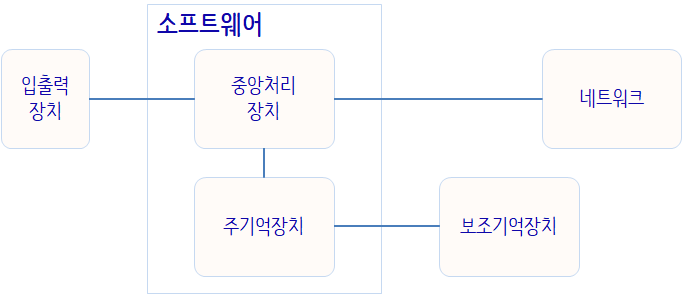
\includegraphics{images/file-arch.png}

}

\caption{\label{fig-software-architecture}소프트웨어 아키텍처}

\end{figure}%

이번 장에서 보조 기억장치(Secondary Memory) 혹은 파일을 가지고 작업을
시작한다. 보조 기억장치는 전원이 꺼져도 지워지지 않는다. 혹은, USB
플래시 드라이브를 사용한 경우에는 프로그램으로부터 작성한 데이터는
시스템에서 제거되어 다른 시스템으로 전송될 수 있다.

우선 텍스트 편집기로 작성한 텍스트 파일을 읽고 쓰는 것에 초점을 맞출
것이다. 나중에 데이터베이스 소프트웨어를 통해서 읽고 쓰도록 설계된
바이너리 파일 데이터베이스를 가지고 어떻게 작업하는지를 살펴볼 것이다.

\section{파일 열기}\label{r-file-open}

\index{파일!열기} \index{열기 함수} \index{함수!열기}

하드 디스크 파일을 읽거나 쓰려고 할 때, 파일을 열어야(open) 한다. 파일을
열 때 각 파일 데이터가 어디에 저장되었는지를 알고 있는 운영체제와
커뮤니케이션한다. 파일을 열 때, 운영체제에 파일이 존재하는지 확인하고
이름으로 파일을 찾도록 요청한다.\\
이번 예제에서, \textless www.py4inf.com/code/mbox.txt\textgreater 에서
파일을 다운로드한 후 R을 시작한 동일한 폴더에 저장된 \texttt{mbox.txt}
파일을 연다.

\texttt{download.file("https://www.dr-chuck.com/py4inf/code/mbox.txt",\ destfile\ =\ "mbox.txt")}
명령어를 사용하여 코딩을 시작하는 디렉토리에 \texttt{mbox.txt} 이름으로
저장한다.

\subsection{R}

\begin{Shaded}
\begin{Highlighting}[]
\NormalTok{\#| label: r{-}file{-}open}
\NormalTok{download.file("https://www.dr{-}chuck.com/py4inf/code/mbox.txt", }
\NormalTok{              destfile = "mbox.txt")}
\NormalTok{fhand \textless{}{-} file("mbox.txt", open = "r")}
\NormalTok{fhand}
\NormalTok{\#\textgreater{} A connection with                           }
\NormalTok{\#\textgreater{} description "mbox.txt"}
\NormalTok{\#\textgreater{} class       "file"         }
\NormalTok{\#\textgreater{} mode        "r"            }
\NormalTok{\#\textgreater{} text        "text"         }
\NormalTok{\#\textgreater{} opened      "opened"       }
\NormalTok{\#\textgreater{} can read    "yes"          }
\NormalTok{\#\textgreater{} can write   "no"  }
\end{Highlighting}
\end{Shaded}

\subsection{파이썬}

\begin{Shaded}
\begin{Highlighting}[]
\NormalTok{\#| label: py{-}file{-}open}
\NormalTok{fhand = open(\textquotesingle{}mbox.txt\textquotesingle{})}
\NormalTok{print(fhand)}
\NormalTok{\#\textgreater{} \textless{}\_io.TextIOWrapper name=\textquotesingle{}mbox.txt\textquotesingle{} mode=\textquotesingle{}r\textquotesingle{} encoding=\textquotesingle{}cp949\textquotesingle{}\textgreater{}}
\end{Highlighting}
\end{Shaded}

\texttt{open}이 성공하면, 운영체제는 \textbf{파일 핸들(file handle)}을
반환한다. 파일 핸들(file handle)은 파일에 담겨진 실제 데이터는 아니고,
대신에 데이터를 읽을 수 있도록 사용할 수 있는 ``핸들(handle)''이다.
요청한 파일이 존재하고, 파일을 읽을 수 있는 적절한 권한이 있다면 이제
핸들이 여러분에게 주어졌다. \index{파일 핸들}

\begin{figure}

\centering{

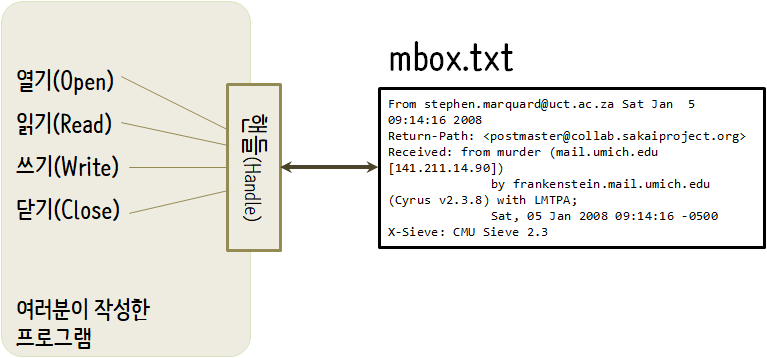
\includegraphics{images/file-handler.png}

}

\caption{\label{fig-file-handler}파일 핸들}

\end{figure}%

파일이 존재하지 않는다면, open은 역추적(traceback) 파일 열기 오류로
실패하고, 파일 콘텐츠에 접근할 핸들도 얻지 못한다.

\subsection{R}

\begin{Shaded}
\begin{Highlighting}[]
\NormalTok{\#| label: r{-}file{-}open{-}error}
\NormalTok{fhand \textless{}{-} file("stuff.txt", "r")}
\NormalTok{\#\textgreater{} file("stuff.txt", "r")에서 다음과 같은 에러가 발생했습니다:커넥션을 열 수 없습니다}
\NormalTok{\#\textgreater{} 추가정보: 경고메시지(들): }
\NormalTok{\#\textgreater{} file("stuff.txt", "r")에서:}
\NormalTok{\#\textgreater{}   파일 \textquotesingle{}stuff.txt\textquotesingle{}를 여는데 실패했습니다: No such file or directory}
\end{Highlighting}
\end{Shaded}

\subsection{파이썬}

\begin{Shaded}
\begin{Highlighting}[]
\NormalTok{\#| label: py{-}file{-}open{-}error}
\NormalTok{fhand = open(\textquotesingle{}stuff.txt\textquotesingle{})}
\NormalTok{\#\textgreater{} Traceback (most recent call last):}
\NormalTok{\#\textgreater{}   File "D:\textbackslash{}tcs\textbackslash{}gpt{-}coding\textbackslash{}file.py", line 1, in \textless{}module\textgreater{}}
\NormalTok{\#\textgreater{}     fhand = open(\textquotesingle{}stuff.txt\textquotesingle{})}
\NormalTok{\#\textgreater{} FileNotFoundError: [Errno 2] No such file or directory: \textquotesingle{}data/stuff.txt\textquotesingle{}}
\end{Highlighting}
\end{Shaded}

나중에 \texttt{tryCatch()}를 가지고, 존재하지 않는 파일을 열려고 하는
상황을 좀 더 우아하게 처리할 것이다. 최근에 사용자 중심으로 R에 다양한
기능이 추가되어 \texttt{tidyverse} 패키지 일부를 구성하는 \texttt{readr}
패키지의 \texttt{read\_lines()} 함수를 통해 인터넷 웹사이트에서 바로
불러오는 것도 가능하다. 하지만, \texttt{readr::read\_lines()} 함수는
줄바꿈 문자를 가정하고 동작하기 때문에 제대로 파일을 못 읽어오는 경우도
종종 있다.

\subsection{R}

\begin{Shaded}
\begin{Highlighting}[]
\NormalTok{\#| label: r{-}file{-}open{-}readLines}
\NormalTok{txt\_file \textless{}{-} readLines("mbox.txt")}

\NormalTok{head(txt\_file)}
\end{Highlighting}
\end{Shaded}

\subsection{파이썬}

\begin{Shaded}
\begin{Highlighting}[]
\NormalTok{\#| label: py{-}file{-}open{-}tidyverse}
\NormalTok{with open("mbox.txt", "r") as f:}
\NormalTok{    txt\_file = f.readlines()}

\NormalTok{for line in txt\_file[:6]:}
\NormalTok{    print(line, end=\textquotesingle{}\textquotesingle{})}
\end{Highlighting}
\end{Shaded}

\section{텍스트 파일과 라인}\label{r-file-txt}

R 문자열이 문자 순서(sequence)로 간주되듯이 마찬가지로 텍스트 파일은
줄(라인, line) 순서(sequence)로 생각될 수 있다. 예를 들어, 다음은 오픈
소스 프로젝트 개발 팀에서 다양한 참여자들의 전자우편 활동을 기록한
텍스트 파일 샘플이다.

\begin{Shaded}
\begin{Highlighting}[]
\NormalTok{From stephen.marquard}\SpecialCharTok{@}\NormalTok{uct.ac.za Sat Jan  }\DecValTok{5} \DecValTok{09}\SpecialCharTok{:}\DecValTok{14}\SpecialCharTok{:}\DecValTok{16} \DecValTok{2008}
\NormalTok{Return}\SpecialCharTok{{-}}\NormalTok{Path}\SpecialCharTok{:} \ErrorTok{\textless{}}\NormalTok{postmaster}\SpecialCharTok{@}\NormalTok{collab.sakaiproject.org}\SpecialCharTok{\textgreater{}}
\NormalTok{Date}\SpecialCharTok{:}\NormalTok{ Sat, }\DecValTok{5}\NormalTok{ Jan }\DecValTok{2008} \DecValTok{09}\SpecialCharTok{:}\DecValTok{12}\SpecialCharTok{:}\DecValTok{18} \SpecialCharTok{{-}}\DecValTok{0500}
\NormalTok{To}\SpecialCharTok{:}\NormalTok{ source}\SpecialCharTok{@}\NormalTok{collab.sakaiproject.org}
\NormalTok{From}\SpecialCharTok{:}\NormalTok{ stephen.marquard}\SpecialCharTok{@}\NormalTok{uct.ac.za}
\NormalTok{Subject}\SpecialCharTok{:}\NormalTok{ [sakai] svn commit}\SpecialCharTok{:}\NormalTok{ r39772 }\SpecialCharTok{{-}}\NormalTok{ content}\SpecialCharTok{/}\NormalTok{branches}\SpecialCharTok{/}
\NormalTok{Details}\SpecialCharTok{:}\NormalTok{ http}\SpecialCharTok{:}\ErrorTok{//}\NormalTok{source.sakaiproject.org}\SpecialCharTok{/}\NormalTok{viewsvn}\SpecialCharTok{/}\NormalTok{?view}\OtherTok{=}\NormalTok{revrev}\OtherTok{=}\DecValTok{39772}
\NormalTok{...}
\end{Highlighting}
\end{Shaded}

상호 의사소통한 전자우편 전체 파일은
\textless www.py4inf.com/code/mbox.txt\textgreater 에서 접근 가능하고,
간략한 버전 파일은
\textless www.py4inf.com/code/mbox-short.txt\textgreater 에서 얻을 수
있다. 이들 파일은 다수 전자우편 메시지를 담고 있는 파일로 표준 포맷으로
되어 있다. ``From''으로 시작하는 라인은 메시지 본문과 구별되고,
``From:''으로 시작하는 라인은 본문 메시지의 일부다. 더 자세한 정보는
\url{http://en.wikipedia.org/wiki/Mbox}에서 찾을 수 있다.

파일을 라인으로 쪼개기 위해서, 줄바꿈 문자로 불리는 ``줄의 끝(end of the
line)''을 표시하는 특수 문자가 있다. \index{줄바꿈}

R에서, 문자열 상수 역슬래시-n(\texttt{\textbackslash{}n})으로 줄바꿈
문자를 표현한다. 두 문자처럼 보이지만, 사실은 단일 문자이다.
인터프리터에 ``stuff''에 입력한 후 변수를 살펴보면, 문자열에
\texttt{\textbackslash{}n}가 있다. 하지만, \texttt{cat}문을 사용하여
문자열을 출력하면, 문자열이 새줄 문자에 의해서 두 줄로 쪼개지는 것을 볼
수 있다.

\subsection{R}

\begin{Shaded}
\begin{Highlighting}[]
\NormalTok{\#| label: r{-}file{-}newline}
\NormalTok{stuff \textless{}{-} \textquotesingle{}Hello\textbackslash{}nWorld!\textquotesingle{}}
\NormalTok{stuff}
\NormalTok{\#\textgreater{} [1] "Hello\textbackslash{}nWorld!"}
\NormalTok{print(stuff)}
\NormalTok{\#\textgreater{} [1] "Hello\textbackslash{}nWorld!"}
\NormalTok{stuff \textless{}{-} \textquotesingle{}X\textbackslash{}nY\textquotesingle{}}
\NormalTok{print(stuff)}
\NormalTok{\#\textgreater{} [1] "X\textbackslash{}nY"}
\NormalTok{str\_length(stuff)}
\NormalTok{\#\textgreater{} [1] 3}
\end{Highlighting}
\end{Shaded}

\subsection{파이썬}

\begin{Shaded}
\begin{Highlighting}[]
\NormalTok{\#| label: py{-}file{-}newline}
\NormalTok{stuff = \textquotesingle{}Hello\textbackslash{}nWorld!\textquotesingle{}}
\NormalTok{stuff}
\NormalTok{\#\textgreater{} \textquotesingle{}Hello\textbackslash{}nWorld!\textquotesingle{}}
\NormalTok{print(stuff)}
\NormalTok{\#\textgreater{} Hello}
\NormalTok{\#\textgreater{} World!}
\NormalTok{stuff = \textquotesingle{}X\textbackslash{}nY\textquotesingle{}}
\NormalTok{print(stuff)}
\NormalTok{\#\textgreater{} X}
\NormalTok{\#\textgreater{} Y}
\NormalTok{len(stuff)}
\NormalTok{\#\textgreater{} 3}
\end{Highlighting}
\end{Shaded}

문자열 \texttt{X\textbackslash{}nY}의 길이는
\texttt{stringr::str\_length("X\textbackslash{}nY")} 명령어를 통해
확인이 가능한데 3이다. 왜냐하면 줄바꿈(newline) 문자도 한 문자이기
때문이다.

그래서, 파일 라인을 볼 때, 라인 끝을 표시하는 줄바꿈으로 불리는 눈에
보이지 않는 특수 문자가 각 줄의 끝에 있다고 상상할 필요가 있다.

그래서, 줄바꿈 문자는 파일에 있는 문자를 라인으로 분리한다.

\section{파일 읽어오기}\label{r-file-open-handler}

\index{파일!읽어 오기} \index{계수기}

파일 핸들(file handle)이 파일 자료를 담고 있지 않지만, for 루프를
사용하여 파일 각 라인을 읽고 라인 수를 세는 것을 쉽게 구축할 수 있다.

\subsection{R}

\begin{Shaded}
\begin{Highlighting}[]
\NormalTok{\#| label: r{-}file{-}open{-}count}
\NormalTok{fhand \textless{}{-} file(\textquotesingle{}mbox.txt\textquotesingle{}, open = "r")}
\NormalTok{count \textless{}{-} 0}

\NormalTok{for(line in readLines(fhand)) \{}
\NormalTok{  count \textless{}{-} count + 1}
\NormalTok{\}}

\NormalTok{message(\textquotesingle{}행수:\textquotesingle{}, count, "\textbackslash{}n")}
\NormalTok{\#\textgreater{} 행수:132045}
\NormalTok{close(fhand)}
\end{Highlighting}
\end{Shaded}

\subsection{파이썬}

\begin{Shaded}
\begin{Highlighting}[]
\NormalTok{\#| label: py{-}file{-}open{-}count}
\NormalTok{fhand = open(\textquotesingle{}mbox.txt\textquotesingle{})}
\NormalTok{count = 0}

\NormalTok{for line in fhand:}
\NormalTok{    count = count + 1}

\NormalTok{print(\textquotesingle{}행수:\textquotesingle{}, count)}
\NormalTok{\#\textgreater{} 행수: 132045}
\end{Highlighting}
\end{Shaded}

파일 핸들을 \texttt{for} 루프 시퀀스(sequence)로 사용할 수 있다.
\texttt{for} 루프는 단순히 파일 라인 수를 세고 전체 라인 수를 출력한다.
\texttt{for} 루프를 대략 일반어로 풀어 말하면, ``파일 핸들로 표현되는
파일 각 라인마다, \texttt{count} 변수에 1씩 더한다.''

\texttt{file} 함수가 전체 파일을 바로 읽지 못하는 이유는 파일이 수
기가바이트(GB) 파일 크기를 가질 수도 있기 때문이다. \texttt{file} 문장은
파일 크기에 관계없이 파일을 여는 데 시간이 동일하게 걸린다. 실질적으로
\texttt{for} 루프가 파일로부터 자료를 읽어오는 역할을 한다.

\texttt{for} 루프를 사용해서 이같은 방식으로 파일을 읽어올 때, 줄바꿈
문자를 사용해서 파일 자료를 라인 단위로 쪼갠다. 파이썬에서 줄바꿈
문자까지 각 라인 단위로 읽고, \texttt{for} 루프가 매번 반복할 때마다
line변수에 줄바꿈을 마지막 문자로 포함한다.

\texttt{for} 루프가 데이터를 한 번에 한 줄씩 읽어오기 때문에, 데이터를
저장할 주기억장치 저장공간을 소진하지 않고, 매우 큰 파일을 효과적으로
읽어서 라인을 셀 수 있다. 각 라인별로 읽고, 세고, 그리고 나서 폐기되기
때문에, 매우 적은 저장공간을 사용해서 어떤 크기의 파일도 상기 프로그램을
사용하여 라인을 셀 수 있다.

만약 주기억장치 크기에 비해서 상대적으로 작은 크기의 파일이라는 것을
안다면, 전체 파일을 파일 핸들로 \texttt{readLines()} 함수를 사용해서
문자열로 읽어올 수 있다.

\subsection{R}

\begin{Shaded}
\begin{Highlighting}[]
\NormalTok{\#| label: r{-}file{-}input}
\NormalTok{download.file("https://www.dr{-}chuck.com/py4inf/code/mbox{-}short.txt",}
\NormalTok{              destfile = "mbox{-}short.txt")}

\NormalTok{fhand \textless{}{-} file("mbox{-}short.txt", open = "r")}
\NormalTok{inp \textless{}{-} readLines(fhand)}
\NormalTok{inp\_str \textless{}{-} paste(inp, collapse = "\textbackslash{}n")}
\NormalTok{close(fhand)}

\NormalTok{print(nchar(inp\_str))}
\NormalTok{\#\textgreater{} [1] 94626}
\NormalTok{print(substr(inp\_str, 1, 20))}
\NormalTok{\#\textgreater{} [1] "From stephen.marquar"}
\end{Highlighting}
\end{Shaded}

\subsection{파이썬}

\begin{Shaded}
\begin{Highlighting}[]
\NormalTok{\#| label: py{-}file{-}input}
\NormalTok{fhand = open(\textquotesingle{}mbox{-}short.txt\textquotesingle{})}
\NormalTok{inp = fhand.read()}
\NormalTok{print(len(inp))}
\NormalTok{\#\textgreater{} 94626}
\NormalTok{print(inp[:20])}
\NormalTok{\#\textgreater{} From stephen.marquar}
\end{Highlighting}
\end{Shaded}

상기 예제에서, \texttt{mbox-short.txt} 전체 파일 콘텐츠(94,626 문자)를
변수 \texttt{inp}로 바로 읽었다. 문자열 슬라이싱을 사용해서
\texttt{inp}에 저장된 문자열 자료 첫 20 문자를 출력한다.

파일이 이런 방식으로 읽혀질 때, 모든 라인과 줄바꿈 문자를 포함한 모든
문자는 변수 \texttt{inp}에 대입된 매우 큰 문자열이다. 파일 데이터가
컴퓨터 주기억장치가 안정적으로 감당해 낼 수 있을 때만, 이런 형식의
\texttt{nchar()} 함수가 사용될 수 있다는 것을 기억하라.

만약 주기억장치가 감당해 낼 수 없는 매우 파일 크기가 크다면,
\texttt{for}나 \texttt{while} 루프를 사용해서 파일을 쪼개서 읽는
프로그램을 작성해야 한다.

\section{파일 검색}\label{r-file-search}

\index{필터 패턴} \index{패턴!필터}

파일 데이터를 검색할 때, 흔한 패턴은 파일을 읽고, 대부분 라인은
건너뛰고, 특정 기준을 만족하는 라인만 처리하는 것이다. 간단한 검색
메커니즘을 구현하기 위해서 파일을 읽는 패턴과 문자열 메서드를 조합한다.

예를 들어, 파일을 읽고, ``From:''으로 시작하는 라인만 출력하고자 한다면,
\texttt{stringr} 패키지에 포함된 \texttt{str\_detect()} 문자열 탐지
함수를 사용해서 원하는 접두사(From:)로 시작하는 라인만을 선택한다.

\subsection{R}

\begin{Shaded}
\begin{Highlighting}[]
\NormalTok{\#| label: r{-}file{-}print{-}from}
\NormalTok{fhand \textless{}{-} readLines("mbox{-}short.txt")}

\NormalTok{for(line in fhand) \{}
\NormalTok{  if(startsWith(line, "From:")) \{}
\NormalTok{    print(line)}
\NormalTok{  \}}
\NormalTok{\}}
\end{Highlighting}
\end{Shaded}

\subsection{파이썬}

\begin{Shaded}
\begin{Highlighting}[]
\NormalTok{\#| label: py{-}file{-}print{-}from}
\NormalTok{fhand = open(\textquotesingle{}mbox{-}short.txt\textquotesingle{})}
\NormalTok{for line in fhand:}
\NormalTok{    if line.startswith(\textquotesingle{}From:\textquotesingle{}) :}
\NormalTok{        print(line)}
\end{Highlighting}
\end{Shaded}

이 프로그램이 실행하면 다음 출력값을 얻는다.

\begin{Shaded}
\begin{Highlighting}[]
\NormalTok{[}\DecValTok{1}\NormalTok{] }\StringTok{"From: stephen.marquard@uct.ac.za"}
\NormalTok{[}\DecValTok{1}\NormalTok{] }\StringTok{"From: louis@media.berkeley.edu"}
\NormalTok{[}\DecValTok{1}\NormalTok{] }\StringTok{"From: zqian@umich.edu"}
\NormalTok{[}\DecValTok{1}\NormalTok{] }\StringTok{"From: rjlowe@iupui.edu"}
\NormalTok{[}\DecValTok{1}\NormalTok{] }\StringTok{"From: zqian@umich.edu"}
\NormalTok{[}\DecValTok{1}\NormalTok{] }\StringTok{"From: rjlowe@iupui.edu"}
\NormalTok{[}\DecValTok{1}\NormalTok{] }\StringTok{"From: cwen@iupui.edu"}
\NormalTok{...}
\end{Highlighting}
\end{Shaded}

``From:''으로만 시작하는 라인만 출력하기 때문에 출력값은 훌륭해 보인다.

파일 처리 프로그램이 점점 더 복잡해짐에 따라 \texttt{next}를 사용해서
검색 루프(search loop)를 구조화할 필요가 있다. 검색 루프의 기본
아이디어는 ``흥미로운'' 라인을 집중적으로 찾고, ``흥미롭지 않은'' 라인은
효과적으로 건너뛰는 것이다. 그리고 나서 흥미로운 라인을 찾게 되면, 그
라인에서 특정 연산을 수행하는 것이다.

다음과 같이 루프를 구성해서 흥미롭지 않은 라인은 건너뛰는 패턴을 따르게
한다.

\subsection{R}

\begin{Shaded}
\begin{Highlighting}[]
\NormalTok{\#| label: r{-}file{-}print{-}from{-}skip}
\NormalTok{fhand \textless{}{-} readLines("mbox{-}short.txt")}

\NormalTok{for (line in fhand) \{}

\NormalTok{  line \textless{}{-} trimws(line, which = "right")}

\NormalTok{  \# 관심 없는 라인 건너뛰기}
\NormalTok{  if (!startsWith(line, "From:")) \{}
\NormalTok{    next}
\NormalTok{  \}}
\NormalTok{  \# 관심 있는 라인 작업}
\NormalTok{  print(line)}
\NormalTok{\}}
\end{Highlighting}
\end{Shaded}

\subsection{파이썬}

\begin{Shaded}
\begin{Highlighting}[]
\NormalTok{\#| label: py{-}file{-}print{-}from{-}skip}
\NormalTok{fhand = open(\textquotesingle{}mbox{-}short.txt\textquotesingle{})}

\NormalTok{for line in fhand:}
\NormalTok{    line = line.rstrip()}
\NormalTok{    \# 관심 없는 라인 건너뛰기}
\NormalTok{    if not line.startswith(\textquotesingle{}From:\textquotesingle{}):}
\NormalTok{        continue}
\NormalTok{    \# 관심 있는 라인 작업}
\NormalTok{    print(line)}
\end{Highlighting}
\end{Shaded}

프로그램의 출력값은 동일하다. 흥미롭지 않는 라인은 ``From:''으로
시작하지 않는 라인이라 \texttt{next}문을 사용해서 건너뛴다. ``흥미로운''
라인(즉, ``From:''으로 시작하는 라인)에 대해서는 연산 처리를 수행한다.

\texttt{str\_detect()} 문자열 함수를 사용해서 검색 문자열이 라인 어디에
있는지를 찾아주는 텍스트 편집기 검색 기능을 모사(simulation)할 수 있다.
\texttt{str\_detect()} 문자열 함수는 다른 문자열 내부에 검색하는
문자열이 있는지 찾고, 존재하는 경우 참(TRUE), 만약 문자열이 없다면
거짓(FALSE)을 반환하기 때문에, ``\textcite{uct.ac.za}''(남아프리카
케이프 타운 대학으로부터 왔다) 문자열을 포함하는 라인을 검색하기 위해
다음과 같이 루프를 작성한다. \texttt{stringr} 패키지 의존성 대신
\texttt{grepl()} 함수를 사용할 수도 있다. \texttt{if}문
\texttt{!str\_detect(line,\ "@uct.ac.za")} 대신
\texttt{grepl("@uct.ac.za",\ line)\ ==\ FALSE}로 대체한다.

\subsection{R}

\begin{Shaded}
\begin{Highlighting}[]
\NormalTok{\#| label: r{-}file{-}find{-}email}
\NormalTok{library(stringr)}

\NormalTok{fhand \textless{}{-} readLines("mbox{-}short.txt")}

\NormalTok{for (line in fhand) \{}
\NormalTok{  line \textless{}{-} trimws(line, which = "right")}
\NormalTok{  if (!str\_detect(line, "@uct.ac.za")) \{}
\NormalTok{    next}
\NormalTok{  \}}
\NormalTok{  print(line)}
\NormalTok{\}}
\end{Highlighting}
\end{Shaded}

\subsection{파이썬}

\begin{Shaded}
\begin{Highlighting}[]
\NormalTok{\#| label: py{-}file{-}find{-}email}
\NormalTok{fhand = open(\textquotesingle{}mbox{-}short.txt\textquotesingle{})}

\NormalTok{for line in fhand:}
\NormalTok{    line = line.rstrip()}
\NormalTok{    if \textquotesingle{}@uct.ac.za\textquotesingle{} not in line:}
\NormalTok{        continue}
\NormalTok{    print(line)}
\end{Highlighting}
\end{Shaded}

출력결과는 다음과 같다.

\begin{Shaded}
\begin{Highlighting}[]
\NormalTok{[}\DecValTok{1}\NormalTok{] }\StringTok{"From stephen.marquard@uct.ac.za Sat Jan  5 09:14:16 2008"}
\NormalTok{[}\DecValTok{1}\NormalTok{] }\StringTok{"X{-}Authentication{-}Warning: nakamura.uits.iupui.edu: apache set sender to stephen.marquard@uct.ac.za using {-}f"}
\NormalTok{[}\DecValTok{1}\NormalTok{] }\StringTok{"From: stephen.marquard@uct.ac.za"}
\NormalTok{[}\DecValTok{1}\NormalTok{] }\StringTok{"Author: stephen.marquard@uct.ac.za"}
\NormalTok{[}\DecValTok{1}\NormalTok{] }\StringTok{"From david.horwitz@uct.ac.za Fri Jan  4 07:02:32 2008"}
\NormalTok{[}\DecValTok{1}\NormalTok{] }\StringTok{"X{-}Authentication{-}Warning: nakamura.uits.iupui.edu: apache set sender to david.horwitz@uct.ac.za using {-}f"}
\NormalTok{[}\DecValTok{1}\NormalTok{] }\StringTok{"From: david.horwitz@uct.ac.za"}
\NormalTok{[}\DecValTok{1}\NormalTok{] }\StringTok{"Author: david.horwitz@uct.ac.za"}
\NormalTok{[}\DecValTok{1}\NormalTok{] }\StringTok{"r39753 | david.horwitz@uct.ac.za | 2008{-}01{-}04 13:05:51 +0200 (Fri, 04 Jan 2008) | 1 line"}
\NormalTok{[}\DecValTok{1}\NormalTok{] }\StringTok{"From david.horwitz@uct.ac.za Fri Jan  4 06:08:27 2008"}
\NormalTok{[}\DecValTok{1}\NormalTok{] }\StringTok{"X{-}Authentication{-}Warning: nakamura.uits.iupui.edu: apache set sender to david.horwitz@uct.ac.za using {-}f"}
\end{Highlighting}
\end{Shaded}

\section{사용자가 파일명 선택}\label{r-file-user-input}

매번 다른 파일을 처리할 때마다 R 코드를 편집하고 싶지는 않다. 매번
프로그램이 실행될 때마다, 파일명을 사용자가 입력하도록 만드는 것이 좀 더
유용할 것이다. 그래서 R 코드를 바꾸지 않고, 다른 파일에 대해서도 동일한
프로그램을 사용하도록 만들자.

다음과 같이 \texttt{commandArgs}을 사용해서 사용자로부터 파일명을 읽어
프로그램을 실행하는 것이 단순하다. \texttt{file-user-input.R} 파일에
다음과 같이 R 스크립트를 작성한다. 자세한 사항은
\href{http://statkclee.github.io/parallel-r/}{R 병렬 프로그래밍}을
참조한다. \footnote{\href{http://statkclee.github.io/parallel-r/r-parallel-rscript-args.html}{.R
  스크립트를 인자와 함께 실행}} 그리고, 사용자의 입력을 받도록 하는
프롬프트를 생략하고 바로 쉘에서 인자를 넘기는 것으로 프로그램을
작성했다.

\subsection*{R}\label{r-38}
\addcontentsline{toc}{subsection}{R}

\begin{Shaded}
\begin{Highlighting}[]
\FunctionTok{cat}\NormalTok{(}\StringTok{"Enter the file name: "}\NormalTok{)}
\NormalTok{fname }\OtherTok{\textless{}{-}} \FunctionTok{readLines}\NormalTok{(}\FunctionTok{file}\NormalTok{(}\StringTok{"stdin"}\NormalTok{), }\DecValTok{1}\NormalTok{) }

\NormalTok{fhand }\OtherTok{\textless{}{-}} \FunctionTok{readLines}\NormalTok{(fname)}

\NormalTok{count }\OtherTok{\textless{}{-}} \DecValTok{0}

\ControlFlowTok{for}\NormalTok{ (line }\ControlFlowTok{in}\NormalTok{ fhand) \{}
  \ControlFlowTok{if}\NormalTok{ (}\FunctionTok{startsWith}\NormalTok{(line, }\StringTok{"Subject:"}\NormalTok{)) \{}
\NormalTok{    count }\OtherTok{\textless{}{-}}\NormalTok{ count }\SpecialCharTok{+} \DecValTok{1}
\NormalTok{  \}}
\NormalTok{\}}

\FunctionTok{print}\NormalTok{(}\FunctionTok{paste}\NormalTok{(}\StringTok{\textquotesingle{}There were\textquotesingle{}}\NormalTok{, count, }\StringTok{\textquotesingle{}subject lines in\textquotesingle{}}\NormalTok{, fname))}
\end{Highlighting}
\end{Shaded}

\subsection*{파이썬}\label{uxd30cuxc774uxc36c-38}
\addcontentsline{toc}{subsection}{파이썬}

\begin{Shaded}
\begin{Highlighting}[]
\NormalTok{fname }\OperatorTok{=} \BuiltInTok{input}\NormalTok{(}\StringTok{\textquotesingle{}Enter the file name: \textquotesingle{}}\NormalTok{)}
\NormalTok{fhand }\OperatorTok{=} \BuiltInTok{open}\NormalTok{(fname)}
\NormalTok{count }\OperatorTok{=} \DecValTok{0}
\ControlFlowTok{for}\NormalTok{ line }\KeywordTok{in}\NormalTok{ fhand:}
    \ControlFlowTok{if}\NormalTok{ line.startswith(}\StringTok{\textquotesingle{}Subject:\textquotesingle{}}\NormalTok{):}
\NormalTok{        count }\OperatorTok{+=} \DecValTok{1}
\BuiltInTok{print}\NormalTok{(}\StringTok{\textquotesingle{}There were\textquotesingle{}}\NormalTok{, count, }\StringTok{\textquotesingle{}subject lines in\textquotesingle{}}\NormalTok{, fname)}
\end{Highlighting}
\end{Shaded}

사용자로부터 파일명을 읽고 변수 \texttt{fname}에 저장하고, 그 파일을
연다. 이제 다른 파일에 대해서도 반복적으로 프로그램을 실행할 수 있다.
RStudio \texttt{Terminal}(\texttt{Console} 패널 아님)을 열고 다음과 같이
인자를 넘겨 실행하면 된다.

\begin{Shaded}
\begin{Highlighting}[]
\SpecialCharTok{$}\NormalTok{ rscript file}\SpecialCharTok{{-}}\NormalTok{user}\SpecialCharTok{{-}}\NormalTok{input.R}
\NormalTok{Enter the file name}\SpecialCharTok{:}\NormalTok{ mbox.txt}
\NormalTok{경고메시지(들)}\SpecialCharTok{:}
\NormalTok{사용되지 않는 커넥션 }\DecValTok{3}\NormalTok{ (stdin)를 닫습니다}
\NormalTok{[}\DecValTok{1}\NormalTok{] }\StringTok{"There were 1797 subject lines in mbox.txt"}

\SpecialCharTok{$}\NormalTok{ rscript file}\SpecialCharTok{{-}}\NormalTok{user}\SpecialCharTok{{-}}\NormalTok{input.R}
\NormalTok{Enter the file name}\SpecialCharTok{:}\NormalTok{ mbox}\SpecialCharTok{{-}}\NormalTok{short.txt}
\NormalTok{경고메시지(들)}\SpecialCharTok{:}
\NormalTok{사용되지 않는 커넥션 }\DecValTok{3}\NormalTok{ (stdin)를 닫습니다}
\NormalTok{[}\DecValTok{1}\NormalTok{] }\StringTok{"There were 27 subject lines in mbox{-}short.txt"}
\NormalTok{There were }\DecValTok{27}\NormalTok{ subject lines }\ControlFlowTok{in}\NormalTok{ ..}\SpecialCharTok{/}\NormalTok{data}\SpecialCharTok{/}\NormalTok{mbox}\SpecialCharTok{{-}}\NormalTok{short.txt}
\end{Highlighting}
\end{Shaded}

다음 절을 살펴보기 전에, 이 프로그램을 검토하면서 자신에게 다음을
질문해보자. ``여기서 무엇이 잘못될 수 있을까?'' 또는 ``이 간결하고 멋진
프로그램이 오류를 발생시키고 바로 종료되어 사용자에게 나쁜 인상을 남길
수 있게 만드는 것은 무엇일까?''

\section{\texorpdfstring{\texttt{tryCatch}
사용하기}{tryCatch 사용하기}}\label{r-file-trycatch}

여러분에게 엿보지 말라고 말씀드렸다. 이번이 마지막 기회다. 사용자가
파일명이 아닌 뭔가 다른 것을 입력하면 어떻게 될까?

\begin{Shaded}
\begin{Highlighting}[]
\SpecialCharTok{$}\NormalTok{ rscript file}\SpecialCharTok{{-}}\NormalTok{user}\SpecialCharTok{{-}}\NormalTok{input.R }\StringTok{"missing.txt"}
\FunctionTok{file}\NormalTok{(con, }\StringTok{"r"}\NormalTok{)에서 다음과 같은 에러가 발생했습니다}\SpecialCharTok{:}\NormalTok{커넥션을 열 수 없습니다}
\NormalTok{호출}\SpecialCharTok{:}\NormalTok{ readLines }\OtherTok{{-}\textgreater{}}\NormalTok{ file}
\NormalTok{추가정보}\SpecialCharTok{:}\NormalTok{ 경고메시지(들)}\SpecialCharTok{:}
\FunctionTok{file}\NormalTok{(con, }\StringTok{"r"}\NormalTok{)에서}\SpecialCharTok{:}
\NormalTok{  파일 }\StringTok{\textquotesingle{}missing.txt\textquotesingle{}}\NormalTok{를 여는데 실패했습니다}\SpecialCharTok{:}\NormalTok{ No such file or directory}
\NormalTok{실행이 정지되었습니다}

\SpecialCharTok{$}\NormalTok{ rscript file}\SpecialCharTok{{-}}\NormalTok{user}\SpecialCharTok{{-}}\NormalTok{input.R }\StringTok{"na na boo boo"}
\FunctionTok{file}\NormalTok{(con, }\StringTok{"r"}\NormalTok{)에서 다음과 같은 에러가 발생했습니다}\SpecialCharTok{:}\NormalTok{커넥션을 열 수 없습니다}
\NormalTok{호출}\SpecialCharTok{:}\NormalTok{ readLines }\OtherTok{{-}\textgreater{}}\NormalTok{ file}
\NormalTok{추가정보}\SpecialCharTok{:}\NormalTok{ 경고메시지(들)}\SpecialCharTok{:}
\FunctionTok{file}\NormalTok{(con, }\StringTok{"r"}\NormalTok{)에서}\SpecialCharTok{:}
\NormalTok{  파일 }\StringTok{\textquotesingle{}na na boo boo\textquotesingle{}}\NormalTok{를 여는데 실패했습니다}\SpecialCharTok{:}\NormalTok{ No such file or directory}
\NormalTok{실행이 정지되었습니다}
\end{Highlighting}
\end{Shaded}

웃을 일은 절대 아니다. 사용자는 결국 여러분이 작성한 프로그램을
망가뜨리기 위해 고의든 악의를 가지든 가능한 모든 수단을 강구할 것이다.
사실, 소프트웨어 개발팀의 중요한 부분은 \textbf{품질 보증(Quality
Assurance, QA)}이라는 조직이다. 품질보증 조직은 프로그래머가 만든
소프트웨어를 망가뜨리기 위해 가능한 말도 안 되는 것을 수행한다.
\index{품질 보증} \index{QA}

사용자가 소프트웨어를 제품으로 구매하거나, 주문형으로 개발하는
프로그램에 대해 월급을 지급하던지 관계없이 품질보증 조직은 프로그램이
사용자에게 전달되기 전까지 프로그램 오류를 발견할 책임이 있다. 그래서
품질보증 조직은 프로그래머의 최고의 친구다.

프로그램 오류를 찾았기 때문에, \texttt{tryCatch} 구조를 사용해서 오류를
우아하게 고쳐본다. 파일 열기 \texttt{file()} 호출이 잘못될 수 있다고
가정하고, \texttt{file()} 호출이 실패할 때를 대비해서 다음과 같이 복구
코드를 추가한다. \index{try 문장} \index{문장!try}
\index{readLines 함수} \index{함수!readLines} \index{예외!입출력 오류}
\index{입출력 오류}

\subsection{\texorpdfstring{R 파일
\texttt{file-user-input-try.R}}{R 파일 file-user-input-try.R}}\label{r-uxd30cuxc77c-file-user-input-try.r}

\begin{Shaded}
\begin{Highlighting}[]
\FunctionTok{cat}\NormalTok{(}\StringTok{"Enter the file name: "}\NormalTok{)}
\NormalTok{fname }\OtherTok{\textless{}{-}} \FunctionTok{readLines}\NormalTok{(}\FunctionTok{file}\NormalTok{(}\StringTok{"stdin"}\NormalTok{), }\DecValTok{1}\NormalTok{) }

\NormalTok{fileOpened }\OtherTok{\textless{}{-}} \ConstantTok{FALSE}

\NormalTok{result }\OtherTok{\textless{}{-}} \FunctionTok{try}\NormalTok{(\{}
\NormalTok{  fhand }\OtherTok{\textless{}{-}} \FunctionTok{readLines}\NormalTok{(fname)}
\NormalTok{  fileOpened }\OtherTok{\textless{}{-}} \ConstantTok{TRUE}
\NormalTok{\}, }\AttributeTok{silent =} \ConstantTok{TRUE}\NormalTok{)}

\ControlFlowTok{if}\NormalTok{ (}\SpecialCharTok{!}\NormalTok{fileOpened) \{}
  \FunctionTok{cat}\NormalTok{(}\StringTok{"File cannot be opened:"}\NormalTok{, fname, }\StringTok{"}\SpecialCharTok{\textbackslash{}n}\StringTok{"}\NormalTok{)}
  \FunctionTok{q}\NormalTok{(}\StringTok{"no"}\NormalTok{)}
\NormalTok{\}}

\NormalTok{count }\OtherTok{\textless{}{-}} \DecValTok{0}

\ControlFlowTok{for}\NormalTok{ (line }\ControlFlowTok{in}\NormalTok{ fhand) \{}
  \ControlFlowTok{if}\NormalTok{ (}\FunctionTok{startsWith}\NormalTok{(line, }\StringTok{"Subject:"}\NormalTok{)) \{}
\NormalTok{    count }\OtherTok{\textless{}{-}}\NormalTok{ count }\SpecialCharTok{+} \DecValTok{1}
\NormalTok{  \}}
\NormalTok{\}}

\FunctionTok{cat}\NormalTok{(}\StringTok{"There were"}\NormalTok{, count, }\StringTok{"subject lines in"}\NormalTok{, fname, }\StringTok{"}\SpecialCharTok{\textbackslash{}n}\StringTok{"}\NormalTok{)}
\end{Highlighting}
\end{Shaded}

\subsection{\texorpdfstring{파이썬
\texttt{file-user-input-try.py}}{파이썬 file-user-input-try.py}}\label{uxd30cuxc774uxc36c-file-user-input-try.py}

\begin{Shaded}
\begin{Highlighting}[]
\NormalTok{fname }\OperatorTok{=} \BuiltInTok{input}\NormalTok{(}\StringTok{\textquotesingle{}Enter the file name: \textquotesingle{}}\NormalTok{)}
\ControlFlowTok{try}\NormalTok{:}
\NormalTok{    fhand }\OperatorTok{=} \BuiltInTok{open}\NormalTok{(fname)}
\ControlFlowTok{except}\NormalTok{:}
    \BuiltInTok{print}\NormalTok{(}\StringTok{\textquotesingle{}File cannot be opened:\textquotesingle{}}\NormalTok{, fname)}
\NormalTok{    exit()}

\NormalTok{count }\OperatorTok{=} \DecValTok{0}
\ControlFlowTok{for}\NormalTok{ line }\KeywordTok{in}\NormalTok{ fhand:}
    \ControlFlowTok{if}\NormalTok{ line.startswith(}\StringTok{\textquotesingle{}Subject:\textquotesingle{}}\NormalTok{):}
\NormalTok{        count }\OperatorTok{+=} \DecValTok{1}

\BuiltInTok{print}\NormalTok{(}\StringTok{\textquotesingle{}There were\textquotesingle{}}\NormalTok{, count, }\StringTok{\textquotesingle{}subject lines in\textquotesingle{}}\NormalTok{, fname)}
\end{Highlighting}
\end{Shaded}

이제 사용자 혹은 품질 보증 조직에서 올바르지 않거나 어처구니없는
파일명을 입력했을 때, 버그를 \texttt{try()} 함수로 잡아서 우아하게
복구한다.

\begin{Shaded}
\begin{Highlighting}[]
\SpecialCharTok{$}\NormalTok{ rscript file}\SpecialCharTok{{-}}\NormalTok{user}\SpecialCharTok{{-}}\NormalTok{input}\SpecialCharTok{{-}}\NormalTok{try.R}
\NormalTok{Enter the file name}\SpecialCharTok{:}\NormalTok{ mbox.txt}
\NormalTok{경고메시지(들)}\SpecialCharTok{:}
\NormalTok{사용되지 않는 커넥션 }\DecValTok{3}\NormalTok{ (stdin)를 닫습니다}
\NormalTok{There were }\DecValTok{1797}\NormalTok{ subject lines }\ControlFlowTok{in}\NormalTok{ mbox.txt}

\SpecialCharTok{$}\NormalTok{ rscript file}\SpecialCharTok{{-}}\NormalTok{user}\SpecialCharTok{{-}}\NormalTok{input}\SpecialCharTok{{-}}\NormalTok{try.R}
\NormalTok{Enter the file name}\SpecialCharTok{:}\NormalTok{ no no no}
\NormalTok{경고메시지(들)}\SpecialCharTok{:}
\FunctionTok{file}\NormalTok{(con, }\StringTok{"r"}\NormalTok{)에서}\SpecialCharTok{:}
\NormalTok{  파일 }\StringTok{\textquotesingle{}no no no\textquotesingle{}}\NormalTok{를 여는데 실패했습니다}\SpecialCharTok{:}\NormalTok{ No such file or directory}
\NormalTok{File cannot be opened}\SpecialCharTok{:}\NormalTok{ no no no}
\end{Highlighting}
\end{Shaded}

R 프로그램을 작성할 때 \texttt{readLines()} 파일 열기 호출을 보호하는
것은 \texttt{try()}의 적절한 사용 예제가 된다. ``R 방식(R way)''으로
무언가를 작성할 때, ``알스러운''이라는 용어를 사용한다. 상기 파일을 여는
예제는 알스러운 방식의 좋은 예가 된다고 말한다.

R에 좀 더 자신감이 생기게 되면, 다른 R 프로그래머와 동일한 문제에 대해
두 가지 동치하는 해답을 가지고 어떤 접근법이 좀 더 ``알스러운지''에 대한
현답을 찾는 데도 관여하게 된다.

``좀 더 알스럽게'' 되는 이유는 프로그래밍이 엔지니어링적인 면과 예술적인
면을 동시에 가지고 있기 때문이다. 항상 무언가를 단지 작동하는 것에만
관심이 있지 않고, 프로그램으로 작성한 해결책이 좀 더 우아하고, 다른
동료에 의해서 우아한 것으로 인정되기를 또한 원한다.

\section{파일에 쓰기}\label{r-file-write}

\index{파일!쓰기}

파일에 쓰기 위해서는 두 번째 매개 변수로 `w' 모드로 파일을 열어야 한다.

\subsection*{R}\label{r-39}
\addcontentsline{toc}{subsection}{R}

\begin{Shaded}
\begin{Highlighting}[]
\NormalTok{fout }\OtherTok{\textless{}{-}} \FunctionTok{file}\NormalTok{(}\StringTok{"output.txt"}\NormalTok{, }\StringTok{"w"}\NormalTok{)}
\FunctionTok{print}\NormalTok{(fout)}
\FunctionTok{close}\NormalTok{(fout)}
\end{Highlighting}
\end{Shaded}

\subsection*{파이썬}\label{uxd30cuxc774uxc36c-39}
\addcontentsline{toc}{subsection}{파이썬}

\begin{Shaded}
\begin{Highlighting}[]
\NormalTok{fout }\OperatorTok{=} \BuiltInTok{open}\NormalTok{(}\StringTok{\textquotesingle{}output.txt\textquotesingle{}}\NormalTok{, }\StringTok{\textquotesingle{}w\textquotesingle{}}\NormalTok{)}
\BuiltInTok{print}\NormalTok{(fout)}
\end{Highlighting}
\end{Shaded}

파일이 이미 존재하는데 쓰기 모드에서 파일을 여는 것은 이전 데이터를 모두
지워버리고, 깨끗한 파일 상태에서 다시 시작되니 주의가 필요하다. 만약
파일이 존재하지 않는다면, 새로운 파일이 생성된다.

파일 핸들 객체의 \texttt{writeLines()} 함수는 데이터를 파일에 저장한다.
라인을 끝내고 싶을 때, 명시적으로 줄바꿈 문자를 삽입해서 파일에 쓰도록
라인 끝을 필히 관리해야 한다. \texttt{print}문이 자동적으로 줄바꿈을
추가하듯이 \texttt{writeLines()} 함수도 자동적으로 줄바꿈을 추가한다.
\index{줄바꿈}

\subsection*{R}\label{r-40}
\addcontentsline{toc}{subsection}{R}

\begin{Shaded}
\begin{Highlighting}[]
\NormalTok{fout }\OtherTok{\textless{}{-}} \FunctionTok{file}\NormalTok{(}\StringTok{"output.txt"}\NormalTok{, }\StringTok{"w"}\NormalTok{)}
\NormalTok{line1 }\OtherTok{\textless{}{-}} \StringTok{"This here\textquotesingle{}s the wattle,}\SpecialCharTok{\textbackslash{}n}\StringTok{"}
\FunctionTok{writeLines}\NormalTok{(line1, fout)}
\NormalTok{line2 }\OtherTok{\textless{}{-}} \StringTok{\textquotesingle{}the emblem of our land.}\SpecialCharTok{\textbackslash{}n}\StringTok{\textquotesingle{}}
\FunctionTok{writeLines}\NormalTok{(line2, fout)}
\FunctionTok{close}\NormalTok{(fout)}
\end{Highlighting}
\end{Shaded}

\subsection*{파이썬}\label{uxd30cuxc774uxc36c-40}
\addcontentsline{toc}{subsection}{파이썬}

\begin{Shaded}
\begin{Highlighting}[]
\NormalTok{fout }\OperatorTok{=} \BuiltInTok{open}\NormalTok{(}\StringTok{"output.txt"}\NormalTok{, }\StringTok{"w"}\NormalTok{)}
\NormalTok{line1 }\OperatorTok{=} \StringTok{"This here\textquotesingle{}s the wattle,}\CharTok{\textbackslash{}n}\StringTok{"}
\NormalTok{fout.write(line1)}
\NormalTok{line2 }\OperatorTok{=} \StringTok{\textquotesingle{}the emblem of our land.}\CharTok{\textbackslash{}n}\StringTok{\textquotesingle{}}
\NormalTok{fout.write(line2)}
\NormalTok{fout.close()}
\end{Highlighting}
\end{Shaded}

파일 쓰기가 끝났을 때, 파일을 필히 닫아야 한다. 파일을 닫는 것은 데이터
마지막 비트까지 디스크에 물리적으로 쓰여져서, 전원이 나가더라도 자료가
유실되지 않는 역할을 한다.

파일 읽기로 연 파일을 닫을 수 있지만, 몇 개 파일을 열어놓았다면 약간
단정치 못하게 끝날 수 있다. 왜냐하면 프로그램이 종료될 때 열린 모든
파일이 닫혀졌는지 파이썬이 확인하기 때문이다. 파일에 쓰기를 할 때는,
파일을 명시적으로 닫아서 예기치 못한 일이 발생할 여지를 없애야 한다.

파일에 두 문장을 써넣은 결과는 다음과 같다.

\begin{Shaded}
\begin{Highlighting}[]
\SpecialCharTok{$}\NormalTok{ cat output.txt}
\NormalTok{This here}\StringTok{\textquotesingle{}s the wattle,}

\StringTok{the emblem of our land.}
\end{Highlighting}
\end{Shaded}

\index{close 메서드} \index{메서드!close}

\section{디버깅}\label{r-file-debug}

\index{디버깅} \index{공백}

파일을 읽고 쓸 때, 공백 때문에 종종 문제에 봉착한다. 이런 종류의 오류는
공백, 탭, 줄바꿈이 눈에 보이지 않기 때문에 디버그하기도 쉽지 않다.

\subsection{R}

\begin{Shaded}
\begin{Highlighting}[]
\NormalTok{\#| label: r{-}file{-}debug}
\NormalTok{s \textless{}{-} \textquotesingle{}1 2\textbackslash{}t 3\textbackslash{}n 4\textquotesingle{}}
\NormalTok{print(cat(s))}
\NormalTok{\#\textgreater{} 1 2   3}
\NormalTok{\#\textgreater{}  4NULL}
\end{Highlighting}
\end{Shaded}

\subsection{파이썬}

\begin{Shaded}
\begin{Highlighting}[]
\NormalTok{\#| label: py{-}file{-}debug}
\NormalTok{s = \textquotesingle{}1 2\textbackslash{}t 3\textbackslash{}n 4\textquotesingle{}}
\NormalTok{print(s)}
\NormalTok{\#\textgreater{} 1 2  3}
\NormalTok{\#\textgreater{}  4}
\end{Highlighting}
\end{Shaded}

우선 RStudio IDE의 상단 메뉴에서 Tools -\textgreater{} Global Options
-\textgreater{} Code -\textgreater{} Display -\textgreater{} ``Show
whitespace characters''를 통해 공백문자(whitespace)에 대해 확인할 수
있다.

내장함수 \texttt{dput}이 도움이 될 수 있다. 인자로 임의 객체를 잡아 객체
문자열 표현식으로 반환한다. 문자열 공백문자는 역슬래시 시퀀스로
표현된다. \index{dput 함수} \index{함수!dput} \index{문자열 표현}

\subsection{R}

\begin{Shaded}
\begin{Highlighting}[]
\NormalTok{\#| label: r{-}file{-}debug}
\NormalTok{s \textless{}{-} \textquotesingle{}1 2\textbackslash{}t 3\textbackslash{}n 4\textquotesingle{}}
\NormalTok{dput(s)}
\NormalTok{\#\textgreater{} "1 2\textbackslash{}t 3\textbackslash{}n 4"}
\end{Highlighting}
\end{Shaded}

\subsection{파이썬}

\begin{Shaded}
\begin{Highlighting}[]
\NormalTok{\#| label: py{-}file{-}debug}
\NormalTok{s = \textquotesingle{}1 2\textbackslash{}t 3\textbackslash{}n 4\textquotesingle{}}
\NormalTok{print(repr(s))}
\NormalTok{\#\textgreater{} \textquotesingle{}1 2\textbackslash{}t 3\textbackslash{}n 4\textquotesingle{}}
\end{Highlighting}
\end{Shaded}

여러분이 봉착하는 또 다른 문제는 다른 시스템에서는 라인 끝을 표기하기
위해서 다른 문자를 사용한다는 점이다. 어떤 시스템은
\texttt{\textbackslash{}n}으로 줄바꿈을 표기하고, 다른 시스템은
\texttt{\textbackslash{}r}으로 반환 문자(return character)를 사용한다.
둘 다 모두 사용하는 시스템도 있다. 파일을 다른 시스템으로 이식한다면,
이러한 불일치가 문제를 야기한다. \index{줄 끝 문자}

대부분의 시스템에는 A 포맷에서 B 포맷으로 변환하는 응용프로그램이 있다.
\url{https://en.wikipedia.org/wiki/Newline}에서 응용프로그램을 찾을 수
있고, 좀 더 많은 것을 읽을 수 있다. 물론, 여러분이 직접 프로그램을
작성할 수도 있다.

\section{용어 정의}\label{r-file-terminology}

\begin{itemize}
\tightlist
\item
  \textbf{잡기(catch)}: \texttt{tryCatch} 함수를 사용하여 프로그램이
  예외 상황으로 인해 종료되는 것을 방지하는 과정으로 예외가 발생할 때
  실행할 코드를 지정하고,정상적으로 코드를 계속 실행할 수 있게 한다.
  \index{잡기}
\item
  \textbf{줄바꿈}: 라인 끝을 표기하기 위해 파일이나 문자열에 사용되는
  특수 문자. \index{줄바꿈}
\item
  \textbf{파이썬다움(Pythonic)}: 파이썬에서 우아하게 작동하는 기술.
  ``try와 catch를 사용하는 것은 파일이 없는 경우를 복구하는 파이썬스러운
  방식이다.'' \index{파이썬다음}
\item
  \textbf{품질 보증(Quality Assurance, QA)}: 소프트웨어 제품의 전반적인
  품질을 보증하는 데 집중하는 사람이나 조직. 품질 보증은 소프트웨어
  제품을 시험하고, 제품이 시장에 출시되기 전에 문제를 확인하는 데
  관여한다. \index{품질 보증}
\item
  \textbf{텍스트 파일}: 하드디스크 같은 영구 저장소에 저장된 일련의 문자
  집합. \index{텍스트 파일}
\end{itemize}

\section*{연습문제}\label{r-file-ex}
\addcontentsline{toc}{section}{연습문제}

\markright{연습문제}

\begin{enumerate}
\def\labelenumi{\arabic{enumi}.}
\tightlist
\item
  파일을 읽고 한 줄씩 파일의 내용을 모두 대문자로 출력하는 프로그램을
  작성하세요. 프로그램을 실행하면 다음과 같이 보일 것입니다.
\end{enumerate}

\begin{Shaded}
\begin{Highlighting}[]
\SpecialCharTok{$}\NormalTok{ Rscript shout.R }\StringTok{"mbox{-}short.txt"}

\NormalTok{FROM STEPHEN.MARQUARD}\SpecialCharTok{@}\NormalTok{UCT.AC.ZA SAT JAN }\DecValTok{5} \DecValTok{09}\SpecialCharTok{:}\DecValTok{14}\SpecialCharTok{:}\DecValTok{16} \DecValTok{2008}
\NormalTok{RETURN}\SpecialCharTok{{-}}\NormalTok{PATH}\SpecialCharTok{:} \ErrorTok{\textless{}}\NormalTok{POSTMASTER}\SpecialCharTok{@}\NormalTok{COLLAB.SAKAIPROJECT.ORG}\SpecialCharTok{\textgreater{}}
\NormalTok{RECEIVED}\SpecialCharTok{:}\NormalTok{ FROM }\FunctionTok{MURDER}\NormalTok{ (MAIL.UMICH.EDU [}\DecValTok{141}\NormalTok{.}\DecValTok{211}\NormalTok{.}\FloatTok{14.90}\NormalTok{])}
\NormalTok{BY }\FunctionTok{FRANKENSTEIN.MAIL.UMICH.EDU}\NormalTok{ (CYRUS V2.}\FloatTok{3.8}\NormalTok{) WITH LMTPA;}
\NormalTok{SAT, }\DecValTok{05}\NormalTok{ JAN }\DecValTok{2008} \DecValTok{09}\SpecialCharTok{:}\DecValTok{14}\SpecialCharTok{:}\DecValTok{16} \SpecialCharTok{{-}}\DecValTok{0500}
\end{Highlighting}
\end{Shaded}

\url{http://www.py4inf.com/code/mbox-short.txt}에서 파일을 다운로드
받으세요.

\begin{enumerate}
\def\labelenumi{\arabic{enumi}.}
\setcounter{enumi}{1}
\tightlist
\item
  파일명을 입력받아, 파일을 읽고, 다음 형식의 라인을 찾는 프로그램을
  작성하세요.
\end{enumerate}

\begin{quote}
X-DSPAM-Confidence: \textbf{0.8475}
\end{quote}

``X-DSPAM-Confidence:''로 시작하는 라인을 만나게 되면, 부동 소수점
숫자를 뽑아내기 위해 해당 라인을 별도로 보관하세요. 라인 수를 세고,
라인으로부터 스팸 신뢰값의 총계를 계산하세요. 파일의 끝에 도달했을 때,
평균 스팸 신뢰도를 출력하세요.

\begin{Shaded}
\begin{Highlighting}[]
\SpecialCharTok{$}\NormalTok{ Rscript calc.R }\StringTok{"mbox{-}short.txt"}
\NormalTok{Average spam confidence}\SpecialCharTok{:} \FloatTok{0.750718518519}

\SpecialCharTok{$}\NormalTok{ Rscript calc.R }\StringTok{"mbox.txt"}
\NormalTok{Average spam confidence}\SpecialCharTok{:} \FloatTok{0.894128046745}
\end{Highlighting}
\end{Shaded}

\texttt{mbox.txt}와 \texttt{mbox-short.txt} 파일에 작성한 프로그램을
시험하세요.

\begin{enumerate}
\def\labelenumi{\arabic{enumi}.}
\setcounter{enumi}{2}
\tightlist
\item
  때때로, 프로그래머가 지루해지거나, 약간 재미를 목적으로, 프로그램에
  무해한 부활절 달걀(Easter Egg,
  \url{https://en.wikipedia.org/wiki/Easter_egg_(media)})을 넣습니다.
  사용자가 파일명을 입력하는 프로그램을 변형시켜, 'na na boo boo'로
  파일명을 정확하게 입력했을 때, 재미있는 메시지를 출력하는 프로그램을
  작성하세요. 파일이 존재하거나, 존재하지 않는 다른 모든 파일에 대해서도
  정상적으로 작동해야 합니다. 여기 프로그램을 실행한 견본이 있습니다.
\end{enumerate}

\begin{Shaded}
\begin{Highlighting}[]
\SpecialCharTok{$}\NormalTok{ Rscript egg.R }\StringTok{"mbox.txt"}
\NormalTok{There were }\DecValTok{1797}\NormalTok{ subject lines }\ControlFlowTok{in}\NormalTok{ mbox.txt}

\SpecialCharTok{$}\NormalTok{ Rscript egg.R }\StringTok{"missing.tyxt"}
\NormalTok{File cannot be opened}\SpecialCharTok{:}\NormalTok{ missing.tyxt}

\SpecialCharTok{$}\NormalTok{ Rscript egg.R }\StringTok{"na na boo boo"}
\ConstantTok{NA} \ConstantTok{NA}\NormalTok{ BOO BOO TO YOU }\SpecialCharTok{{-}}\NormalTok{ You have been punk}\StringTok{\textquotesingle{}d!}
\end{Highlighting}
\end{Shaded}

프로그램에 부활절 달걀을 넣도록 격려하지는 않습니다. 단지 연습입니다.

\chapter{리스트}\label{r-list}

\index{리스트} \index{자료형!리스트}

\section{리스트는 시퀀스다}\label{r-list-sequence}

문자열처럼, 리스트(list)는 값의 시퀀스다. 문자열에서, 값은 문자지만,
리스트에서는 임의 자료형(type)도 될 수 있다. 리스트 값은
요소(elements)나 때때로 항목(items)으로 불린다. \index{요소}
\index{시퀀스} \index{항목}

신규 리스트를 생성하는 방법은 여러 가지가 있다. 가장 간단한 방법은
\texttt{list()} 함수로 요소를 감싸는 것이다.

\subsection*{R}\label{r-43}
\addcontentsline{toc}{subsection}{R}

\begin{Shaded}
\begin{Highlighting}[]
\FunctionTok{list}\NormalTok{(}\DecValTok{10}\NormalTok{, }\DecValTok{20}\NormalTok{, }\DecValTok{30}\NormalTok{, }\DecValTok{40}\NormalTok{)}
\FunctionTok{list}\NormalTok{(}\StringTok{\textquotesingle{}crunchy frog\textquotesingle{}}\NormalTok{, }\StringTok{\textquotesingle{}ram bladder\textquotesingle{}}\NormalTok{, }\StringTok{\textquotesingle{}lark vomit\textquotesingle{}}\NormalTok{)}
\FunctionTok{list}\NormalTok{(}\StringTok{\textquotesingle{}고양이\textquotesingle{}}\NormalTok{, }\StringTok{\textquotesingle{}호랑이\textquotesingle{}}\NormalTok{, }\StringTok{\textquotesingle{}사자\textquotesingle{}}\NormalTok{)}
\end{Highlighting}
\end{Shaded}

\subsection*{파이썬}\label{uxd30cuxc774uxc36c-43}
\addcontentsline{toc}{subsection}{파이썬}

\begin{Shaded}
\begin{Highlighting}[]
\NormalTok{[}\DecValTok{10}\NormalTok{, }\DecValTok{20}\NormalTok{, }\DecValTok{30}\NormalTok{, }\DecValTok{40}\NormalTok{]}
\NormalTok{[}\StringTok{\textquotesingle{}crunchy frog\textquotesingle{}}\NormalTok{, }\StringTok{\textquotesingle{}ram bladder\textquotesingle{}}\NormalTok{, }\StringTok{\textquotesingle{}lark vomit\textquotesingle{}}\NormalTok{]}
\NormalTok{[}\StringTok{\textquotesingle{}고양이\textquotesingle{}}\NormalTok{, }\StringTok{\textquotesingle{}호랑이\textquotesingle{}}\NormalTok{, }\StringTok{\textquotesingle{}사자\textquotesingle{}}\NormalTok{]}
\end{Highlighting}
\end{Shaded}

첫 번째 예제는 4개 정수 리스트다. 두번째 예제는 3개 문자열 리스트다. 세
번째 예제는 한글 문자열 리스트다. 리스트 문자열 요소가 동일한
자료형(type)일 필요는 없다. 다음 리스트는 문자열, 부동 소수점 숫자,
정수, (아!) 또 다른 리스트를 담고 있다.

\subsection*{R}\label{r-44}
\addcontentsline{toc}{subsection}{R}

\begin{Shaded}
\begin{Highlighting}[]
\FunctionTok{list}\NormalTok{(}\StringTok{\textquotesingle{}spam\textquotesingle{}}\NormalTok{, }\FloatTok{2.0}\NormalTok{, }\DecValTok{5}\NormalTok{, }\FunctionTok{list}\NormalTok{(}\DecValTok{10}\NormalTok{, }\DecValTok{20}\NormalTok{))}
\end{Highlighting}
\end{Shaded}

\subsection*{파이썬}\label{uxd30cuxc774uxc36c-44}
\addcontentsline{toc}{subsection}{파이썬}

\begin{Shaded}
\begin{Highlighting}[]
\NormalTok{[}\StringTok{\textquotesingle{}spam\textquotesingle{}}\NormalTok{, }\FloatTok{2.0}\NormalTok{, }\DecValTok{5}\NormalTok{, [}\DecValTok{10}\NormalTok{, }\DecValTok{20}\NormalTok{]]}
\end{Highlighting}
\end{Shaded}

또 다른 리스트 내부에 리스트가 \textbf{중첩(nested)}되어 있다.
\index{중첩 리스트} \index{리스트!중첩}

어떤 요소도 담고 있지 않는 리스트를 빈 리스트(empty list)라고 부르고,
\texttt{list()}로 생성한다. \index{빈 리스트} \index{리스트!빈}

예상했듯이, 리스트 값을 변수에 대입할 수 있다.

\subsection{R}

\begin{Shaded}
\begin{Highlighting}[]
\NormalTok{\#| label: r{-}list{-}data}
\NormalTok{cheeses \textless{}{-} list(\textquotesingle{}체다\textquotesingle{}, \textquotesingle{}브리\textquotesingle{}, \textquotesingle{}까망베르\textquotesingle{})}
\NormalTok{numbers \textless{}{-} list(17, 123)}
\NormalTok{empty \textless{}{-} list()}
\NormalTok{message(cheeses, numbers, empty)}
\NormalTok{\#\textgreater{} 체다브리까망베르17123}
\end{Highlighting}
\end{Shaded}

\subsection{파이썬}

\begin{Shaded}
\begin{Highlighting}[]
\NormalTok{\#| label: py{-}list{-}data}
\NormalTok{cheeses = [\textquotesingle{}체다\textquotesingle{}, \textquotesingle{}브리\textquotesingle{}, \textquotesingle{}까망베르\textquotesingle{}]}
\NormalTok{numbers = [17, 123]}
\NormalTok{empty = []}
\NormalTok{print(cheeses, numbers, empty)}
\NormalTok{\#\textgreater{} [\textquotesingle{}체다\textquotesingle{}, \textquotesingle{}브리\textquotesingle{}, \textquotesingle{}까망베르\textquotesingle{}] [17, 123] []}
\end{Highlighting}
\end{Shaded}

\index{대입}

\section{리스트는 변경 가능하다}\label{r-list-mutable}

\index{리스트!요소} \index{접근} \index{인덱스} \index{꺾쇠 연산자}
\index{연산자!꺾쇠}

리스트 요소에 접근하는 구문은 문자열 문자에 접근하는 것과 동일한 꺾쇠
괄호 연산자다. 꺾쇠 괄호 내부 표현식은 인덱스를 명세한다. 기억할 것은
인덱스는 1에서부터 시작한다는 것이다.

\subsection{R}

\begin{Shaded}
\begin{Highlighting}[]
\NormalTok{\#| label: r{-}list{-}access\}}
\NormalTok{cheeses[1]}
\NormalTok{\#\textgreater{} [[1]]}
\NormalTok{\#\textgreater{} [1] "체다"}
\end{Highlighting}
\end{Shaded}

\subsection{파이썬}

\begin{Shaded}
\begin{Highlighting}[]
\NormalTok{\#| label: py{-}list{-}access\}}
\NormalTok{cheeses[0]}
\NormalTok{\#\textgreater{} \textquotesingle{}체다\textquotesingle{}}
\end{Highlighting}
\end{Shaded}

문자열과 마찬가지로, 리스트 항목 순서를 바꾸거나, 리스트에 새로운 항목을
다시 대입할 수 있기 때문에 리스트는 변경 가능하다. 꺾쇠 괄호 연산자가
대입문 왼쪽편에 나타날 때, 새로 대입될 리스트 요소를 나타낸다.
\index{변경성}

\subsection{R}

\begin{Shaded}
\begin{Highlighting}[]
\NormalTok{\#| label: r{-}list{-}mutable}
\NormalTok{numbers \textless{}{-} list(17, 123)}

\NormalTok{numbers[1] \textless{}{-} 5}
\NormalTok{print(numbers)}
\NormalTok{\#\textgreater{} [[1]]}
\NormalTok{\#\textgreater{} [1] 5}
\NormalTok{\#\textgreater{} }
\NormalTok{\#\textgreater{} [[2]]}
\NormalTok{\#\textgreater{} [1] 123}
\end{Highlighting}
\end{Shaded}

\subsection{파이썬}

\begin{Shaded}
\begin{Highlighting}[]
\NormalTok{\#| label: py{-}list{-}mutable}
\NormalTok{numbers = [17, 123]}
\NormalTok{numbers[1] = 5}
\NormalTok{print(numbers)}
\NormalTok{\#\textgreater{} [17, 5]}
\end{Highlighting}
\end{Shaded}

리스트 numbers의 첫 번째 요소는 \texttt{123} 값을 가지고 있었으나, 이제
\texttt{5} 값을 가진다. \index{인덱스!1 에서 시작}
\index{1, 인덱스 시작점}

리스트를 인덱스와 요소의 관계로 생각할 수 있다. 이 관계를
\textbf{매핑(mapping)}이라고 부른다. 각각의 인덱스는 요소 중 하나에
\textbf{대응(``maps to'')}된다. \index{항목 대입} \index{대입!항목}

리스트 인덱스는 문자열 인덱스와 동일한 방식으로 동작한다.

\begin{itemize}
\tightlist
\item
  어떠한 정수 표현식도 인덱스로 사용할 수 있다.
\item
  존재하지 않는 요소를 읽거나 쓰려고 하면, 일종의 인덱스
  오류(IndexError)로 \texttt{NULL}이 반환된다.
\item
  인덱스가 음의 값이면, 해당 리스트 원소가 누락된다.
  \index{예외!인덱스 오류} \index{인덱스 오류}
\end{itemize}

\texttt{\%in\%} 연산자도 또한 리스트에서 동작하니 리스트 원소로
존재하는지 여부를 판별하는 데 사용할 수 있다.

\index{리스트!인덱스} \index{리스트!소속} \index{소속!리스트}
\textbackslash index\{\%in\% 연산자\}
\textbackslash index\{연산자!\%in\%\}

\subsection{R}

\begin{Shaded}
\begin{Highlighting}[]
\NormalTok{\#| label: r{-}list{-}in}
\NormalTok{cheeses \textless{}{-} list(\textquotesingle{}체다\textquotesingle{}, \textquotesingle{}브리\textquotesingle{}, \textquotesingle{}까망베르\textquotesingle{})}
\NormalTok{\textquotesingle{}체다\textquotesingle{} \%in\% cheeses}
\NormalTok{\#\textgreater{} [1] TRUE}
\NormalTok{\textquotesingle{}고르곤졸라\textquotesingle{} \%in\% cheeses}
\NormalTok{\#\textgreater{} [1] FALSE}
\end{Highlighting}
\end{Shaded}

\subsection{파이썬}

\begin{Shaded}
\begin{Highlighting}[]
\NormalTok{\#| label: py{-}list{-}in}
\NormalTok{cheeses = [\textquotesingle{}체다\textquotesingle{}, \textquotesingle{}브리\textquotesingle{}, \textquotesingle{}까망베르\textquotesingle{}]}
\NormalTok{\textquotesingle{}체다\textquotesingle{} in cheeses}
\NormalTok{True}
\NormalTok{\textquotesingle{}고르곤졸라\textquotesingle{} in cheeses}
\NormalTok{False}
\end{Highlighting}
\end{Shaded}

\section{리스트 순회법}\label{r-list-traversal}

\index{리스트!운행법} \index{운행법!리스트} \index{for 루프}
\index{루프!for} \index{문장!for}

리스트 요소를 순회하는 가장 흔한 방법은 \texttt{for} 문을 사용하는
것이다. 문자열에서 사용한 것과 구문은 동일하다.

\subsection*{R}\label{r-49}
\addcontentsline{toc}{subsection}{R}

\begin{Shaded}
\begin{Highlighting}[]
\ControlFlowTok{for}\NormalTok{(cheese }\ControlFlowTok{in}\NormalTok{ cheeses) \{}
  \FunctionTok{print}\NormalTok{(cheese)}
\NormalTok{\}}
\end{Highlighting}
\end{Shaded}

\subsection*{파이썬}\label{uxd30cuxc774uxc36c-49}
\addcontentsline{toc}{subsection}{파이썬}

\begin{Shaded}
\begin{Highlighting}[]
\ControlFlowTok{for}\NormalTok{ cheese }\KeywordTok{in}\NormalTok{ cheeses:}
    \BuiltInTok{print}\NormalTok{ cheese}
\end{Highlighting}
\end{Shaded}

리스트 요소를 읽기만 한다면 이것만으로도 잘 동작한다. 하지만, 리스트
요소를 쓰거나 갱신하는 경우, 인덱스가 필요하다. 리스트 요소를 쓰거나
갱신하는 일반적인 방법은 \texttt{seq\_along()} 함수를 조합하는 것이다.
\index{루프!인덱스} \index{인덱스!루프}

\subsection{R}

\begin{Shaded}
\begin{Highlighting}[]
\NormalTok{\#| label: r{-}list{-}seq\_along}
\NormalTok{numbers \textless{}{-} list(1, 2, 3, 4, 5)}

\NormalTok{for(i in seq\_along(numbers))\{}
\NormalTok{  numbers[[i]] \textless{}{-} numbers[[i]] * 2}
\NormalTok{  message("결과:", numbers[[i]])}
\NormalTok{\}}
\end{Highlighting}
\end{Shaded}

\subsection{파이썬}

\begin{Shaded}
\begin{Highlighting}[]
\NormalTok{\#| label: py{-}list{-}seq\_along}
\NormalTok{numbers = [1, 2, 3, 4, 5]}

\NormalTok{for i in range(len(numbers)):}
\NormalTok{    numbers[i] = numbers[i] * 2}
\NormalTok{    print("결과:", numbers[i])}
\end{Highlighting}
\end{Shaded}

상기 루프는 리스트를 순회하고 각 요소를 갱신한다. \texttt{seq\_along()}
함수는 1에서 \(n\)까지 리스트 인덱스를 반환한다. 여기서, \(n\)은 리스트
길이가 된다. 매번 루프가 반복될 때마다, \texttt{i}는 다음 요소 인덱스를
얻는다. 몸통 부문 대입문은 \texttt{i}를 사용해서 요소의 이전 값을 읽고
새 값을 대입한다. \index{항목 갱신} \index{갱신!항목}

빈 리스트(\texttt{list()})에 대해서 \texttt{for} 문은 결코 몸통 부문을
실행하지 않는다.

\subsection*{R}\label{r-51}
\addcontentsline{toc}{subsection}{R}

\begin{Shaded}
\begin{Highlighting}[]
\ControlFlowTok{for}\NormalTok{(x }\ControlFlowTok{in} \FunctionTok{list}\NormalTok{()) \{}
  \FunctionTok{print}\NormalTok{(}\StringTok{\textquotesingle{}이런 일은 절대 발생하지 않는다.\textquotesingle{}}\NormalTok{)}
\NormalTok{\}}
\end{Highlighting}
\end{Shaded}

\subsection*{파이썬}\label{uxd30cuxc774uxc36c-51}
\addcontentsline{toc}{subsection}{파이썬}

\begin{Shaded}
\begin{Highlighting}[]
\ControlFlowTok{for}\NormalTok{ x }\KeywordTok{in}\NormalTok{ empty:}
    \BuiltInTok{print}\NormalTok{(}\StringTok{\textquotesingle{}이런 일은 절대 발생하지 않는다.\textquotesingle{}}\NormalTok{)}
\end{Highlighting}
\end{Shaded}

리스트가 또 다른 리스트를 담을 수 있지만, 중첩된 리스트는 여전히 요소
하나로 간주된다. 다음 리스트 길이는 4다. \index{중첩 리스트}
\index{리스트!중첩}

\subsection*{R}\label{r-52}
\addcontentsline{toc}{subsection}{R}

\begin{Shaded}
\begin{Highlighting}[]
\FunctionTok{list}\NormalTok{(}\StringTok{\textquotesingle{}spam\textquotesingle{}}\NormalTok{, }\DecValTok{1}\NormalTok{, }\FunctionTok{list}\NormalTok{(}\StringTok{\textquotesingle{}브리\textquotesingle{}}\NormalTok{, }\StringTok{\textquotesingle{}체다\textquotesingle{}}\NormalTok{, }\StringTok{\textquotesingle{}까멩베르\textquotesingle{}}\NormalTok{), }\FunctionTok{list}\NormalTok{(}\DecValTok{1}\NormalTok{, }\DecValTok{2}\NormalTok{, }\DecValTok{3}\NormalTok{))}
\end{Highlighting}
\end{Shaded}

\subsection*{파이썬}\label{uxd30cuxc774uxc36c-52}
\addcontentsline{toc}{subsection}{파이썬}

\begin{Shaded}
\begin{Highlighting}[]
\NormalTok{[}\StringTok{\textquotesingle{}spam\textquotesingle{}}\NormalTok{, }\DecValTok{1}\NormalTok{, [}\StringTok{\textquotesingle{}Brie\textquotesingle{}}\NormalTok{, }\StringTok{\textquotesingle{}Roquefort\textquotesingle{}}\NormalTok{, }\StringTok{\textquotesingle{}Pol le Veq\textquotesingle{}}\NormalTok{], [}\DecValTok{1}\NormalTok{, }\DecValTok{2}\NormalTok{, }\DecValTok{3}\NormalTok{]]}
\end{Highlighting}
\end{Shaded}

\section{리스트 연산자}\label{r-list-operator}

\index{리스트!연산}

\texttt{c()} 함수 연산자는 리스트를 추가하여 결합시킨다.
\index{연결!리스트} \index{리스트!연결}

\subsection{R}

\begin{Shaded}
\begin{Highlighting}[]
\NormalTok{\#| label: r{-}list{-}append}
\NormalTok{a \textless{}{-} list(1, 2, 3)}
\NormalTok{b \textless{}{-} list(4, 5, 6)}
\NormalTok{c \textless{}{-} c(a, b)}
\NormalTok{print(c)}
\end{Highlighting}
\end{Shaded}

\subsection{파이썬}

\begin{Shaded}
\begin{Highlighting}[]
\NormalTok{\#| label: py{-}list{-}append}
\NormalTok{a = [1, 2, 3]}
\NormalTok{b = [4, 5, 6]}
\NormalTok{c = a + b}
\NormalTok{print(c)}
\NormalTok{\#\textgreater{} [1, 2, 3, 4, 5, 6]}
\end{Highlighting}
\end{Shaded}

유사하게 \texttt{rep()} 함수를 활용하면 주어진 횟수만큼 리스트를
반복한다. \index{반복!리스트} \index{리스트!반복}

\subsection{R}

\begin{Shaded}
\begin{Highlighting}[]
\NormalTok{\#| label: r{-}list{-}repeat}
\NormalTok{rep(list(0), 4)}

\NormalTok{rep(list(1, 2, 3), 3)}
\end{Highlighting}
\end{Shaded}

\subsection{파이썬}

\begin{Shaded}
\begin{Highlighting}[]
\NormalTok{\#| label: py{-}list{-}repeat}
\NormalTok{[0] * 4}
\NormalTok{\#\textgreater{} [0, 0, 0, 0]}
\NormalTok{[1, 2, 3] * 3}
\NormalTok{\#\textgreater{} [1, 2, 3, 1, 2, 3, 1, 2, 3]}
\end{Highlighting}
\end{Shaded}

첫 예제는 \texttt{list(0)}을 4회 반복한다. 두 번째 예제는
\texttt{list(1,\ 2,\ 3)} 리스트를 3회 반복한다.

\section{리스트 슬라이스}\label{r-list-slice}

\index{슬라이스 연산자} \index{연산자!슬라이스} \index{인덱스!슬라이스}
\index{리스트!슬라이스} \index{슬라이스!리스트}

\textbf{슬라이스(slice)} 연산자는 리스트에도 또한 동작한다.

\subsection{R}

\begin{Shaded}
\begin{Highlighting}[]
\NormalTok{\#| label: r{-}list{-}slice\}}
\NormalTok{t \textless{}{-} list(\textquotesingle{}a\textquotesingle{}, \textquotesingle{}b\textquotesingle{}, \textquotesingle{}c\textquotesingle{}, \textquotesingle{}d\textquotesingle{}, \textquotesingle{}e\textquotesingle{}, \textquotesingle{}f\textquotesingle{})}

\NormalTok{t[2:3]}

\NormalTok{t[1:4]}

\NormalTok{t[4:length(t)]}

\NormalTok{t}
\end{Highlighting}
\end{Shaded}

\subsection{파이썬}

\begin{Shaded}
\begin{Highlighting}[]
\NormalTok{\#| label: py{-}list{-}slice}
\NormalTok{t = [\textquotesingle{}a\textquotesingle{}, \textquotesingle{}b\textquotesingle{}, \textquotesingle{}c\textquotesingle{}, \textquotesingle{}d\textquotesingle{}, \textquotesingle{}e\textquotesingle{}, \textquotesingle{}f\textquotesingle{}]}
\NormalTok{t[1:3]}
\NormalTok{\#\textgreater{} [\textquotesingle{}b\textquotesingle{}, \textquotesingle{}c\textquotesingle{}]}
\NormalTok{ t[:4]}
\NormalTok{\#\textgreater{} [\textquotesingle{}a\textquotesingle{}, \textquotesingle{}b\textquotesingle{}, \textquotesingle{}c\textquotesingle{}, \textquotesingle{}d\textquotesingle{}]}
\NormalTok{t[3:]}
\NormalTok{\#\textgreater{} [\textquotesingle{}d\textquotesingle{}, \textquotesingle{}e\textquotesingle{}, \textquotesingle{}f\textquotesingle{}]}
\NormalTok{t[:]}
\NormalTok{\#\textgreater{} [\textquotesingle{}a\textquotesingle{}, \textquotesingle{}b\textquotesingle{}, \textquotesingle{}c\textquotesingle{}, \textquotesingle{}d\textquotesingle{}, \textquotesingle{}e\textquotesingle{}, \textquotesingle{}f\textquotesingle{}]}
\end{Highlighting}
\end{Shaded}

첫 번째 인덱스를 1로 지정하면, 슬라이스는 처음부터 시작한다. 두 번째
인덱스를 \texttt{length()} 함수로 리스트 길이를 지정하면, 슬라이스는
끝까지 간다. 그래서 양쪽의 인덱스를 생략하면, \texttt{t}같이 지정하면
슬라이스 결과는 전체 리스트를 복사한 것이 된다. \index{리스트!복사}
\index{슬라이스!복사} \index{복사!슬라이스}

리스트는 변경이 가능하기 때문에 리스트를 접고, 돌리고, 훼손하는 연산을
수행하기 전에 복사본을 만들어두는 것이 유용하다. \index{변경성}

대입문 왼편의 슬라이스 연산자로 복수의 요소를 갱신할 수 있다.
\index{슬라이스!갱신} \index{갱신!슬라이스}

\subsection{R}

\begin{Shaded}
\begin{Highlighting}[]
\NormalTok{\#| label: r{-}list{-}update}
\NormalTok{t \textless{}{-} list(\textquotesingle{}a\textquotesingle{}, \textquotesingle{}b\textquotesingle{}, \textquotesingle{}c\textquotesingle{}, \textquotesingle{}d\textquotesingle{}, \textquotesingle{}e\textquotesingle{}, \textquotesingle{}f\textquotesingle{})}
\NormalTok{t[2:3] \textless{}{-} list(1, 2)}
\NormalTok{print(t)}
\end{Highlighting}
\end{Shaded}

\subsection{파이썬}

\begin{Shaded}
\begin{Highlighting}[]
\NormalTok{\#| label: py{-}list{-}update}
\NormalTok{t = [\textquotesingle{}a\textquotesingle{}, \textquotesingle{}b\textquotesingle{}, \textquotesingle{}c\textquotesingle{}, \textquotesingle{}d\textquotesingle{}, \textquotesingle{}e\textquotesingle{}, \textquotesingle{}f\textquotesingle{}]}
\NormalTok{t[1:3] = [1, 2]}
\NormalTok{print(t)}
\NormalTok{\#\textgreater{} [\textquotesingle{}a\textquotesingle{}, 1, 2, \textquotesingle{}d\textquotesingle{}, \textquotesingle{}e\textquotesingle{}, \textquotesingle{}f\textquotesingle{}]}
\end{Highlighting}
\end{Shaded}

\section{리스트 함수}\label{r-list-function}

\index{리스트!함수} \index{함수, 리스트}

R은 리스트 자료형에 연산할 수 있는 함수를 제공한다. 예를 들어,
덧붙이기(\texttt{append}) 함수는 리스트 끝에 신규 요소를 추가한다.

\subsection{R}

\begin{Shaded}
\begin{Highlighting}[]
\NormalTok{\#| label: r{-}list{-}function{-}append}
\NormalTok{t \textless{}{-} list(\textquotesingle{}a\textquotesingle{}, \textquotesingle{}b\textquotesingle{}, \textquotesingle{}c\textquotesingle{})}
\NormalTok{append(t, \textquotesingle{}d\textquotesingle{})}
\end{Highlighting}
\end{Shaded}

\subsection{파이썬}

\begin{Shaded}
\begin{Highlighting}[]
\NormalTok{\#| label: py{-}list{-}function{-}append\}}
\NormalTok{t = [\textquotesingle{}a\textquotesingle{}, \textquotesingle{}b\textquotesingle{}, \textquotesingle{}c\textquotesingle{}]}
\NormalTok{t.append(\textquotesingle{}d\textquotesingle{})}
\NormalTok{print(t)}
\NormalTok{\#\textgreater{} [\textquotesingle{}a\textquotesingle{}, \textquotesingle{}b\textquotesingle{}, \textquotesingle{}c\textquotesingle{}, \textquotesingle{}d\textquotesingle{}]}
\end{Highlighting}
\end{Shaded}

정렬(order) 함수는 낮음에서 높음으로 리스트 요소를 정렬한다. 리스트에서
\texttt{sapply()} 혹은 \texttt{unlist()} 함수로 값으로 변환시키고
\texttt{order()} 함수를 통해 내림차순 혹은 오름차순으로 정렬 인덱스를
뽑아 리스트 내 원소를 정렬시킨다. \index{정렬 함수} \index{함수!정렬}

\subsection{R}

\begin{Shaded}
\begin{Highlighting}[]
\NormalTok{\#| label: r{-}list{-}function{-}sort}
\NormalTok{t \textless{}{-} list(\textquotesingle{}d\textquotesingle{}, \textquotesingle{}c\textquotesingle{}, \textquotesingle{}e\textquotesingle{}, \textquotesingle{}b\textquotesingle{}, \textquotesingle{}a\textquotesingle{})}

\NormalTok{t[order(unlist(t), decreasing=FALSE)]}
\end{Highlighting}
\end{Shaded}

\subsection{파이썬}

\begin{Shaded}
\begin{Highlighting}[]
\NormalTok{\#| label: py{-}list{-}function{-}sort}
\NormalTok{t = [\textquotesingle{}d\textquotesingle{}, \textquotesingle{}c\textquotesingle{}, \textquotesingle{}e\textquotesingle{}, \textquotesingle{}b\textquotesingle{}, \textquotesingle{}a\textquotesingle{}]}
\NormalTok{t.sort()}
\NormalTok{print(t)}
\NormalTok{\#\textgreater{} [\textquotesingle{}a\textquotesingle{}, \textquotesingle{}b\textquotesingle{}, \textquotesingle{}c\textquotesingle{}, \textquotesingle{}d\textquotesingle{}, \textquotesingle{}e\textquotesingle{}]}
\end{Highlighting}
\end{Shaded}

\section{리스트 요소 삭제}\label{r-list-delete}

\index{리스트 요소 삭제} \index{삭제, 리스트 요소}

리스트 요소를 삭제하는 방법이 몇 가지 있다. 리스트 요소 인덱스를 알고
있다면, 숫자 인덱스 앞에 \texttt{-} 기호를 붙여 사용한다.

\subsection{R}

\begin{Shaded}
\begin{Highlighting}[]
\NormalTok{\#| label: r{-}list{-}delete{-}by{-}index}
\NormalTok{t \textless{}{-} list(\textquotesingle{}a\textquotesingle{}, \textquotesingle{}b\textquotesingle{}, \textquotesingle{}c\textquotesingle{})}
\NormalTok{x \textless{}{-} t[2]}
\NormalTok{t \textless{}{-} t[{-}2]}
\NormalTok{print(x)}
\NormalTok{print(t)}
\end{Highlighting}
\end{Shaded}

\subsection{파이썬}

\begin{Shaded}
\begin{Highlighting}[]
\NormalTok{\#| label: py{-}list{-}delete{-}by{-}index}
\NormalTok{t = [\textquotesingle{}a\textquotesingle{}, \textquotesingle{}b\textquotesingle{}, \textquotesingle{}c\textquotesingle{}]}
\NormalTok{x = t.pop(1)}
\NormalTok{print(t)}
\NormalTok{\#\textgreater{} [\textquotesingle{}a\textquotesingle{}, \textquotesingle{}c\textquotesingle{}]}
\NormalTok{print(x)}
\NormalTok{\#\textgreater{} b}
\end{Highlighting}
\end{Shaded}

리스트 요소 명칭을 알고 있다면, 리스트 요소에 \texttt{NULL}을 대입하여
삭제시킨다.

\begin{Shaded}
\begin{Highlighting}[]
\NormalTok{t }\OtherTok{\textless{}{-}} \FunctionTok{list}\NormalTok{(}\AttributeTok{a=}\StringTok{\textquotesingle{}a\textquotesingle{}}\NormalTok{, }\AttributeTok{b=}\StringTok{\textquotesingle{}b\textquotesingle{}}\NormalTok{, }\AttributeTok{c =} \StringTok{\textquotesingle{}c\textquotesingle{}}\NormalTok{)}
\NormalTok{t[[}\StringTok{"c"}\NormalTok{]] }\OtherTok{\textless{}{-}} \ConstantTok{NULL}
\NormalTok{t}\SpecialCharTok{$}\NormalTok{c }\OtherTok{\textless{}{-}} \ConstantTok{NULL}
\NormalTok{t}
\CommentTok{\#\textgreater{} $a}
\CommentTok{\#\textgreater{} [1] "a"}
\CommentTok{\#\textgreater{} }
\CommentTok{\#\textgreater{} $b}
\CommentTok{\#\textgreater{} [1] "b"}
\end{Highlighting}
\end{Shaded}

\texttt{NULL}을 대입하여 삭제시킨 리스트는 제거된 요소를 반환한다.
\texttt{t{[}{[}1{]}{]}} 리스트 인덱스를 통해 요소에 접근하고
\texttt{NULL}을 대입하여 삭제한다. \index{NULL 특수값}
\index{특수값!NULL}

\subsection{R}

\begin{Shaded}
\begin{Highlighting}[]
\NormalTok{\#| label: r{-}list{-}delete{-}by{-}index}
\NormalTok{t = list(\textquotesingle{}a\textquotesingle{}, \textquotesingle{}b\textquotesingle{}, \textquotesingle{}c\textquotesingle{})}
\NormalTok{t[[1]] \textless{}{-} NULL}
\NormalTok{t}
\end{Highlighting}
\end{Shaded}

\subsection{파이썬}

\begin{Shaded}
\begin{Highlighting}[]
\NormalTok{\#| label: py{-}list{-}delete{-}by{-}index}
\NormalTok{t = [\textquotesingle{}a\textquotesingle{}, \textquotesingle{}b\textquotesingle{}, \textquotesingle{}c\textquotesingle{}]}
\NormalTok{del t[1]}
\NormalTok{print(t)}
\NormalTok{\#\textgreater{} [\textquotesingle{}a\textquotesingle{}, \textquotesingle{}c\textquotesingle{}]}
\end{Highlighting}
\end{Shaded}

(인덱스 혹은 리스트 요소 이름이 아닌) 제거할 요소값을 알고 있다면,
리스트 요소 값을 활용해서 제거하는 것도 가능하다.

\subsection{R}

\begin{Shaded}
\begin{Highlighting}[]
\NormalTok{\#| label: r{-}list{-}delete{-}by{-}value}
\NormalTok{t \textless{}{-} list(\textquotesingle{}x\textquotesingle{}, \textquotesingle{}y\textquotesingle{}, \textquotesingle{}z\textquotesingle{})}

\NormalTok{t[t != "y"]}
\end{Highlighting}
\end{Shaded}

\subsection{파이썬}

\begin{Shaded}
\begin{Highlighting}[]
\NormalTok{\#| label: py{-}list{-}delete{-}by{-}value}
\NormalTok{t = [\textquotesingle{}a\textquotesingle{}, \textquotesingle{}b\textquotesingle{}, \textquotesingle{}c\textquotesingle{}]}
\NormalTok{t.remove(\textquotesingle{}b\textquotesingle{})}
\NormalTok{print(t)}
\NormalTok{\#\textgreater{} [\textquotesingle{}a\textquotesingle{}, \textquotesingle{}c\textquotesingle{}]}
\end{Highlighting}
\end{Shaded}

하나 이상의 요소를 제거하기 위해서, 슬라이스 인덱스(slice index)를
사용하는 것도 가능하다.

\subsection{R}

\begin{Shaded}
\begin{Highlighting}[]
\NormalTok{\#| label: r{-}list{-}delete{-}slice}
\NormalTok{t \textless{}{-} list(\textquotesingle{}a\textquotesingle{}, \textquotesingle{}b\textquotesingle{}, \textquotesingle{}c\textquotesingle{}, \textquotesingle{}d\textquotesingle{}, \textquotesingle{}e\textquotesingle{}, \textquotesingle{}f\textquotesingle{})}
\NormalTok{t[{-}c(2:5)]}
\end{Highlighting}
\end{Shaded}

\subsection{파이썬}

\begin{Shaded}
\begin{Highlighting}[]
\NormalTok{\#| label: py{-}list{-}delete{-}slice}
\NormalTok{t = [\textquotesingle{}a\textquotesingle{}, \textquotesingle{}b\textquotesingle{}, \textquotesingle{}c\textquotesingle{}, \textquotesingle{}d\textquotesingle{}, \textquotesingle{}e\textquotesingle{}, \textquotesingle{}f\textquotesingle{}]}
\NormalTok{del t[1:5]}
\NormalTok{print(t)}
\NormalTok{\#\textgreater{} [\textquotesingle{}a\textquotesingle{}, \textquotesingle{}f\textquotesingle{}]}
\end{Highlighting}
\end{Shaded}

위의 예제에서 2에서 5까지 모든 요소를 선택하고 선택된 모든 요소를
제거한다.

\section{리스트와 함수}\label{uxb9acuxc2a4uxd2b8uxc640-uxd568uxc218}

루프를 작성하지 않고도 리스트를 빠르게 살펴볼 수 있는 리스트에 적용할 수
있는 내장 함수를 활용하는 것도 방법이지만, 깔끔한 세상(tidyverse)
생태계의 일원인 \texttt{purrr} 함수형 프로그래밍 패키지에 내장된 함수를
활용하는 것도 권장된다.

하지만, 다음과 같이 1차원 리스트는 \texttt{unlist()} 함수를 활용하여
벡터로 변환해서 사용하는 것이 편리한 경우가 많다.

\subsection{R}

\begin{Shaded}
\begin{Highlighting}[]
\NormalTok{\#| label: r{-}list{-}unlist}
\NormalTok{nums \textless{}{-} list(3, 41, 12, 9, 74, 15) \%\textgreater{}\% unlist}

\NormalTok{length(nums)}
\NormalTok{\#\textgreater{} 6}
\NormalTok{max(nums)}
\NormalTok{\#\textgreater{} 74}
\NormalTok{min(nums)}
\NormalTok{\#\textgreater{} 3}
\NormalTok{sum(nums)}
\NormalTok{\#\textgreater{} 154}
\NormalTok{sum(nums) / length(nums)}
\NormalTok{\#\textgreater{} 25.66667}
\end{Highlighting}
\end{Shaded}

\subsection{파이썬}

\begin{Shaded}
\begin{Highlighting}[]
\NormalTok{\#| label: py{-}list{-}unlist}
\NormalTok{nums = [3, 41, 12, 9, 74, 15]}

\NormalTok{print(len(nums))}
\NormalTok{\#\textgreater{} 6}
\NormalTok{print(max(nums))}
\NormalTok{\#\textgreater{} 74}
\NormalTok{print(min(nums))}
\NormalTok{\#\textgreater{} 3  }
\NormalTok{print(sum(nums))}
\NormalTok{\#\textgreater{} 154  }
\NormalTok{print(sum(nums) / len(nums))}
\NormalTok{\#\textgreater{} 25.666666666666668}
\end{Highlighting}
\end{Shaded}

\texttt{sum()}, \texttt{max()}, \texttt{length()} 등 함수는 입력
자료형이 무엇이냐에 따라 다르게 동작할 수 있고, 입력 자료형에 결측값 등
특이값이 들어있는 경우 기대했던 결과가 나올 수 없으니 반드시 자료형을
사전에 점검하고 활용하도록 한다.

리스트를 사용해서, 앞서 작성한 프로그램을 다시 작성해서 사용자가 입력한
숫자 목록 평균을 계산한다.

우선 리스트 없이 평균을 계산하는 프로그램:

\subsection{R}

\begin{Shaded}
\begin{Highlighting}[]
\NormalTok{\#| label: r{-}list{-}user{-}input{-}average}
\NormalTok{\#\# 프로그램 명칭: \textasciigrave{}list\_average.R\textasciigrave{}}
\NormalTok{total \textless{}{-} 0}
\NormalTok{count \textless{}{-} 0}

\NormalTok{while(TRUE) \{}
\NormalTok{  cat("숫자를 입력하세요: ")}
\NormalTok{  inp \textless{}{-} readLines(file("stdin"), 1)}
\NormalTok{  if(inp == \textquotesingle{}done\textquotesingle{}) \{}
\NormalTok{    break}
\NormalTok{  \}}
\NormalTok{  value \textless{}{-} as.numeric(inp)}
\NormalTok{  total \textless{}{-} total + value}
\NormalTok{  count \textless{}{-} count + 1}
\NormalTok{\}}

\NormalTok{average \textless{}{-} total / count}
\NormalTok{message(\textquotesingle{}평균:\textquotesingle{}, average)}
\NormalTok{\#\textgreater{} 숫자를 입력하세요: 10}
\NormalTok{\#\textgreater{} 숫자를 입력하세요: 20}
\NormalTok{\#\textgreater{} 숫자를 입력하세요: 30}
\NormalTok{\#\textgreater{} 숫자를 입력하세요: done}
\NormalTok{\#\textgreater{} 평균: 20}
\end{Highlighting}
\end{Shaded}

\subsection{파이썬}

\begin{Shaded}
\begin{Highlighting}[]
\NormalTok{\#| label: py{-}list{-}user{-}input{-}average}
\NormalTok{total = 0}
\NormalTok{count = 0}

\NormalTok{while True:}
\NormalTok{    inp = input(\textquotesingle{}숫자를 입력하세요: \textquotesingle{})}
\NormalTok{    if inp == \textquotesingle{}done\textquotesingle{}:}
\NormalTok{        break}
\NormalTok{    value = float(inp)}
\NormalTok{    total += value}
\NormalTok{    count += 1}

\NormalTok{average = total / count}
\NormalTok{print(\textquotesingle{}평균:\textquotesingle{}, average)}

\NormalTok{\#\textgreater{} 숫자를 입력하세요: 10}
\NormalTok{\#\textgreater{} 숫자를 입력하세요: 20}
\NormalTok{\#\textgreater{} 숫자를 입력하세요: 30}
\NormalTok{\#\textgreater{} 숫자를 입력하세요: done}
\NormalTok{\#\textgreater{} 평균: 20.0}
\end{Highlighting}
\end{Shaded}

상기 프로그램에서, \texttt{count} 와 \texttt{sum} 변수를 사용해서
반복적으로 사용자가 숫자를 입력하면 값을 저장하고, 지금까지 사용자가
입력한 누적 합계를 계산한다. R 콘솔에서 \texttt{source()} 함수를
사용해서 실행한 결과는 다음과 같다.

\begin{Shaded}
\begin{Highlighting}[]
\SpecialCharTok{\textgreater{}} \FunctionTok{source}\NormalTok{(}\StringTok{"code/list\_average.R"}\NormalTok{)}
\NormalTok{숫자를 입력하세요}\SpecialCharTok{:} \DecValTok{10}
\NormalTok{숫자를 입력하세요}\SpecialCharTok{:} \DecValTok{20}
\NormalTok{숫자를 입력하세요}\SpecialCharTok{:} \DecValTok{30}
\NormalTok{숫자를 입력하세요}\SpecialCharTok{:}\NormalTok{ done}
\NormalTok{평균}\SpecialCharTok{:} \DecValTok{20}
\end{Highlighting}
\end{Shaded}

단순하게, 사용자가 입력한 각 숫자를 리스트로 기억하고 내장 함수를
사용해서 프로그램 마지막에 합계와 갯수를 통해 평균을 계산한다.

\subsection{R}

\begin{Shaded}
\begin{Highlighting}[]
\NormalTok{\#| label: r{-}list{-}user{-}input{-}average}
\NormalTok{\# list\_average2.R ... 자료구조 사용 }
\NormalTok{numlist \textless{}{-} list()}

\NormalTok{while(TRUE) \{}
\NormalTok{  cat("숫자를 입력하세요: ")}
\NormalTok{  inp \textless{}{-} readLines(file("stdin"), 1)}
\NormalTok{  if(inp == \textquotesingle{}done\textquotesingle{}) \{}
\NormalTok{    break}
\NormalTok{  \}}
\NormalTok{  value \textless{}{-} as.numeric(inp)}
\NormalTok{  numlist \textless{}{-} append(numlist, value)}
\NormalTok{\}}

\NormalTok{average \textless{}{-} sum(unlist(numlist)) / length(numlist)}
\NormalTok{message(\textquotesingle{}평균:\textquotesingle{}, average)}
\end{Highlighting}
\end{Shaded}

\subsection{파이썬}

\begin{Shaded}
\begin{Highlighting}[]
\NormalTok{\#| label: py{-}list{-}user{-}input{-}average}
\NormalTok{numlist = list()}

\NormalTok{while True:}
\NormalTok{    inp = input(\textquotesingle{}숫자를 입력하세요: \textquotesingle{})}
\NormalTok{    if inp == \textquotesingle{}done\textquotesingle{}:}
\NormalTok{        break}
\NormalTok{    value = float(inp)}
\NormalTok{    numlist.append(value)}

\NormalTok{average = sum(numlist) / len(numlist)}
\NormalTok{print(\textquotesingle{}평균:\textquotesingle{}, average)}
\end{Highlighting}
\end{Shaded}

루프가 시작되기 전 빈 리스트를 생성하고, 매번 숫자를 입력할 때마다
숫자를 리스트에 추가한다. 프로그램 마지막에 간단하게 리스트 총합을
계산하고, 평균을 산출하기 위해서 입력한 숫자 개수로 나눈다. R 콘솔에서
\texttt{source()} 함수를 사용해서 실행한 결과는 다음과 같다.

\begin{Shaded}
\begin{Highlighting}[]
\OperatorTok{\textgreater{}}\NormalTok{ source}\KeywordTok{(}\StringTok{"code/list\_average2.R"}\KeywordTok{)}
\ExtensionTok{숫자를}\NormalTok{ 입력하세요: 10}
\ExtensionTok{숫자를}\NormalTok{ 입력하세요: 20}
\ExtensionTok{숫자를}\NormalTok{ 입력하세요: 30}
\ExtensionTok{숫자를}\NormalTok{ 입력하세요: done}
\ExtensionTok{평균:}\NormalTok{ 20}
\end{Highlighting}
\end{Shaded}

\section{리스트와 문자열}\label{r-list-string}

\index{리스트} \index{문자열} \index{시퀀스}

문자열(string)은 \textbf{문자 시퀀스}이고, 리스트는 \textbf{값
시퀀스}이다. 하지만 리스트 문자는 문자열과 같지는 않다. 문자열을 리스트
문자로 변환하기 위해서, \texttt{strsplit()} 함수를 사용한다.
\index{리스트!함수} \index{함수!리스트}

\subsection{R}

\begin{Shaded}
\begin{Highlighting}[]
\NormalTok{\#| label: py{-}list{-}strsplit}
\NormalTok{s \textless{}{-} \textquotesingle{}spam\textquotesingle{}}
\NormalTok{t \textless{}{-} strsplit(s, "")[[1]] |\textgreater{}  strsplit(NULL)}
\NormalTok{print(t)}
\end{Highlighting}
\end{Shaded}

\subsection{파이썬}

\begin{Shaded}
\begin{Highlighting}[]
\NormalTok{\#| label: r{-}list{-}strsplit}
\NormalTok{s = \textquotesingle{}spam\textquotesingle{}}
\NormalTok{t = list(s)}
\NormalTok{print(t)}
\NormalTok{\#\textgreater{} [\textquotesingle{}s\textquotesingle{}, \textquotesingle{}p\textquotesingle{}, \textquotesingle{}a\textquotesingle{}, \textquotesingle{}m\textquotesingle{}]}
\end{Highlighting}
\end{Shaded}

\texttt{list}는 내장 함수 이름이기 때문에, 변수명으로 사용하는 것을
피해야 한다. \texttt{l}을 사용하면 1처럼 보이기 때문에 가능하면 피한다.
그래서, \texttt{t}를 사용했다.

\texttt{strsplit()} 함수는 문자열을 구분자(이번 경우에는
\texttt{NULL})를 사용해서 문자 각각으로 쪼갠다. 문자열 단어로 쪼개려면,
구분자를 바꿔 예를 들어 공백을 기준으로 쪼갠다. \index{분할 함수}
\index{함수!분할}

\subsection{R}

\begin{Shaded}
\begin{Highlighting}[]
\NormalTok{\#| label: r{-}list{-}split{-}separator}
\NormalTok{s \textless{}{-} list(\textquotesingle{}이제는 디지털 글쓰기가 대세다.\textquotesingle{})}
\NormalTok{t \textless{}{-} strsplit(s[[1]], " ")[[1]] \%\textgreater{}\% strsplit(" ")}
\NormalTok{t}
\end{Highlighting}
\end{Shaded}

\subsection{파이썬}

\begin{Shaded}
\begin{Highlighting}[]
\NormalTok{\#| label: py{-}list{-}split{-}separator}
\NormalTok{s = \textquotesingle{}이제는 디지털 글쓰기가 대세다.\textquotesingle{}}
\NormalTok{t = s.split()}
\NormalTok{print(t)}
\NormalTok{\#\textgreater{} [\textquotesingle{}이제는\textquotesingle{}, \textquotesingle{}디지털\textquotesingle{}, \textquotesingle{}글쓰기가\textquotesingle{}, \textquotesingle{}대세다.\textquotesingle{}]}
\end{Highlighting}
\end{Shaded}

분할 함수를 사용해서 문자열을 리스트 토큰으로 쪼개면, 인덱스
연산자(`{[}{]}')를 사용하여 리스트의 특정 단어를 볼 수 있다.

옵션 인자로 단어 경계로 어떤 문자를 사용할 것인지 지정하는 데 사용되는
구분자(delimiter)를 활용하여 분할 \texttt{strsplit()} 함수를 호출한다.
다음 예제는 구분자로 하이픈(`-')을 사용한 사례이다. \index{옵션 인자}
\index{인자!옵션} \index{구분자}

\subsection{R}

\begin{Shaded}
\begin{Highlighting}[]
\NormalTok{\#| label: r{-}list{-}delimiter}
\NormalTok{s \textless{}{-} list(\textquotesingle{}spam{-}spam{-}spam\textquotesingle{})}
\NormalTok{delimiter \textless{}{-} \textquotesingle{}{-}\textquotesingle{}}
\NormalTok{strsplit(s[[1]], delimiter)[[1]] \%\textgreater{}\% strsplit(" ")}
\end{Highlighting}
\end{Shaded}

\subsection{파이썬}

\begin{Shaded}
\begin{Highlighting}[]
\NormalTok{\#| label: py{-}list{-}delimiter}
\NormalTok{s = \textquotesingle{}spam{-}spam{-}spam\textquotesingle{}}
\NormalTok{delimiter = \textquotesingle{}{-}\textquotesingle{}}
\NormalTok{print(s.split(delimiter))}
\NormalTok{\#\textgreater{} [\textquotesingle{}spam\textquotesingle{}, \textquotesingle{}spam\textquotesingle{}, \textquotesingle{}spam\textquotesingle{}]}
\end{Highlighting}
\end{Shaded}

합병(\texttt{paste}) 함수는 분할(\texttt{strsplit}) 함수의 역이다.
문자열 리스트를 받아 리스트 요소를 연결한다. \index{합병 함수}
\index{합병!paste} \index{연결}

\subsection{R}

\begin{Shaded}
\begin{Highlighting}[]
\NormalTok{\#| label: r{-}list{-}paste}
\NormalTok{t \textless{}{-} list(\textquotesingle{}이제는\textquotesingle{}, \textquotesingle{}디지털\textquotesingle{}, \textquotesingle{}글쓰기가\textquotesingle{}, \textquotesingle{}대세다.\textquotesingle{})}
\NormalTok{delimiter \textless{}{-} \textquotesingle{} \textquotesingle{}}
\NormalTok{paste0(t, delimiter, collapse = "")}
\NormalTok{\#\textgreater{} [1] "이제는 디지털 글쓰기가 대세다. "}
\end{Highlighting}
\end{Shaded}

\subsection{파이썬}

\begin{Shaded}
\begin{Highlighting}[]
\NormalTok{\#| label: py{-}list{-}paste}
\NormalTok{t = [\textquotesingle{}이제는\textquotesingle{}, \textquotesingle{}디지털\textquotesingle{}, \textquotesingle{}글쓰기가\textquotesingle{}, \textquotesingle{}대세다.\textquotesingle{}]}
\NormalTok{delimiter = \textquotesingle{} \textquotesingle{}}
\NormalTok{print(delimiter.join(t))}
\NormalTok{\#\textgreater{} 이제는 디지털 글쓰기가 대세다.}
\end{Highlighting}
\end{Shaded}

상기의 경우, 구분자가 공백 문자여서 결합(\texttt{paste}) 함수가 단어
사이에 공백을 넣는다. 공백 없이 문자열을 결합하기 위해서, 구분자로 빈
문자열 '\,'을 사용한다. \index{빈 문자열} \index{문자열!빈}

\section{라인 파싱하기}\label{r-list-parsing}

파일을 읽을 때 통상, 단지 전체 라인을 출력하는 것 말고 뭔가 다른 것을
하고자 한다. 종종 ``흥미로운 라인을'' 찾아서 라인을
\textbf{파싱(parse)}하여 흥미로운 부분을 찾고자 한다. ``From''으로
시작하는 라인에서 요일을 찾고자 하면 어떨까?

\begin{quote}
\texttt{From\ stephen.marquard@uct.ac.za} \textbf{Sat}
\texttt{Jan\ \ 5\ 09:14:16\ 2008}
\end{quote}

이런 종류의 문제에 직면했을 때, \texttt{stringr} 패키지 분할
\texttt{str\_split()} 함수가 매우 효과적이다. 작은 프로그램을 작성하여
``From''으로 시작하는 라인을 찾고 \texttt{str\_split()} 함수로 파싱하고
라인의 흥미로운 부분을 출력한다.

\subsection{R}

\begin{Shaded}
\begin{Highlighting}[]
\NormalTok{\#| label: r{-}list{-}email{-}parsing}
\NormalTok{download.file("https://www.dr{-}chuck.com/py4inf/code/mbox{-}short.txt",}
\NormalTok{              destfile = "mbox{-}short.txt")}

\NormalTok{fhand \textless{}{-} readLines(\textquotesingle{}mbox{-}short.txt\textquotesingle{})}

\NormalTok{for (line in fhand) \{}
\NormalTok{    line \textless{}{-} trimws(line)  \# 공백 제거}
\NormalTok{    if (length(grep("\^{}From ", line)) == 0) \{}
\NormalTok{        next}
\NormalTok{    \}}
\NormalTok{    words \textless{}{-} unlist(strsplit(line, " "))}
\NormalTok{    if (length(words) \textgreater{}= 3) \{}
\NormalTok{        print(words[3])}
\NormalTok{    \}}
\NormalTok{\}}
\end{Highlighting}
\end{Shaded}

\subsection{파이썬}

\begin{Shaded}
\begin{Highlighting}[]
\NormalTok{\#| label: py{-}list{-}email{-}parsing}
\NormalTok{fhand = open(\textquotesingle{}mbox{-}short.txt\textquotesingle{})}

\NormalTok{for line in fhand:}
\NormalTok{    line = line.rstrip()}
\NormalTok{    if not line.startswith(\textquotesingle{}From \textquotesingle{}):}
\NormalTok{        continue}
\NormalTok{    words = line.split()}
\NormalTok{    print(words[2])}
\end{Highlighting}
\end{Shaded}

\texttt{if} 문의 축약 형태를 사용하여 \texttt{next} 문을 \texttt{if}
문과 동일한 라인에 놓았다. \texttt{if} 문 축약 형태는 \texttt{next} 문을
들여쓰기를 다음 라인에 한 것과 동일하다.

프로그램은 다음을 출력한다.

\begin{Shaded}
\begin{Highlighting}[]
\ExtensionTok{Sat}
\ExtensionTok{Fri}
\ExtensionTok{Fri}
\ExtensionTok{Fri}
\ExtensionTok{...}
\end{Highlighting}
\end{Shaded}

나중에, 매우 정교한 기술에 대해서 학습해서 정확하게 검색하는 비트(bit)
수준 정보를 찾아내기 위해서 작업할 라인을 선택하고, 어떻게 해당 라인을
뽑아낼 것이다.

\section{객체와 값}\label{r-list-object-value}

\index{객체} \index{값}

다음 대입문을 실행하면,

\begin{Shaded}
\begin{Highlighting}[]
\NormalTok{a }\OtherTok{\textless{}{-}} \StringTok{\textquotesingle{}banana\textquotesingle{}}
\NormalTok{b }\OtherTok{\textless{}{-}} \StringTok{\textquotesingle{}banana\textquotesingle{}}
\end{Highlighting}
\end{Shaded}

\texttt{a}와 \texttt{b} 모두 문자열을 참조하지만, 두 변수가 동일한
문자열을 참조하는지 알 수 없다. 두 가지 가능한 상태가 있다.

\begin{figure}

\centering{

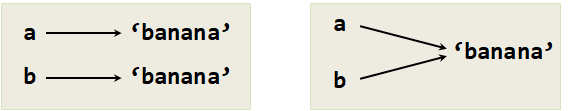
\includegraphics{images/list-reference.png}

}

\caption{\label{fig-list-reference}문자열 참조}

\end{figure}%

한 가지 경우는 \texttt{a}와 \texttt{b}가 같은 값을 가지는 다른 두 객체를
참조하는 것이다. 두 번째 경우는 같은 객체를 참조하는 것이다.
\index{에일리어싱}

두 변수가 동일한 객체를 참조하는지를 확인하기 위해서, 파이썬에서는
\texttt{is} 연산자가 사용된다.

\subsection{R}

\begin{Shaded}
\begin{Highlighting}[]
\NormalTok{\#| label: r{-}a{-}b{-}reference}
\NormalTok{a \textless{}{-} \textquotesingle{}banana\textquotesingle{}}
\NormalTok{b \textless{}{-} \textquotesingle{}banana\textquotesingle{}}
\NormalTok{print(identical(a, b))}
\NormalTok{\#\textgreater{} [1] TRUE}
\end{Highlighting}
\end{Shaded}

\subsection{파이썬}

\begin{Shaded}
\begin{Highlighting}[]
\NormalTok{\#| label: py{-}a{-}b{-}reference}
\NormalTok{a = \textquotesingle{}banana\textquotesingle{}}
\NormalTok{b = \textquotesingle{}banana\textquotesingle{}}
\NormalTok{print(a is b)}
\NormalTok{\#\textgreater{} True}
\end{Highlighting}
\end{Shaded}

이 경우, 파이썬은 하나의 문자열 객체를 생성하고 \texttt{a}와 \texttt{b}
모두 동일한 객체를 참조한다. \index{동일 연산자}
\index{연산자!identical}

하지만, 리스트 두 개를 생성할 때, 객체가 두 개다.

\subsection{R}

\begin{Shaded}
\begin{Highlighting}[]
\NormalTok{\#| label: r{-}a{-}b{-}list}
\NormalTok{a \textless{}{-} list(1, 2, 3)}
\NormalTok{b \textless{}{-} list(1, 2, 3)}
\NormalTok{print(identical(a, b))}
\end{Highlighting}
\end{Shaded}

\subsection{파이썬}

\begin{Shaded}
\begin{Highlighting}[]
\NormalTok{\#| label: py{-}a{-}b{-}list}
\NormalTok{a = [1, 2, 3]}
\NormalTok{b = [1, 2, 3]}
\NormalTok{print(a is b)}
\NormalTok{\#\textgreater{} False}
\end{Highlighting}
\end{Shaded}

상기의 경우, 두 개의 리스트는 동등하다고 말할 수 있다. 왜냐하면 동일한
요소를 가지고 있기 때문이다. 하지만, 같은 객체는 아니기 때문에
동일하지는 않다. 두 개의 객체가 동일하다면, 두 객체는 또한 동등하다.
하지만, 동등하다고 해서 반드시 동일하지는 않다. \index{동등}
\index{동일}

R과 파이썬이 다른 결과를 출력하는 이유는 무엇일까? R
\texttt{identical()} 함수는 객체의 값과 구조가 완전히 동일한지를
확인한다. \texttt{a\ \textless{}-\ list(1,\ 2,\ 3)}와
\texttt{b\ \textless{}-\ list(1,\ 2,\ 3)}의 경우, \texttt{a}와
\texttt{b}는 별도의 객체이지만, 그 내용(값과 구조)이 완전히 동일하기
때문에 \texttt{identical(a,\ b)}는 \texttt{TRUE}를 반환한다. 파이썬
\texttt{is} 연산자는 객체가 메모리 상에서 동일한 위치를 가리키는지(즉,
같은 객체인지)를 확인한다. \texttt{a\ =\ {[}1,\ 2,\ 3{]}}와
\texttt{b\ =\ {[}1,\ 2,\ 3{]}}의 경우, \texttt{a}와 \texttt{b}는 값은
동일하지만 서로 다른 메모리 위치에 할당된 별개의 리스트 객체라서
\texttt{a\ is\ b}는 \texttt{False}를 반환한다.

지금까지 ``객체(object)''와 ``값(value)''을 구분 없이 사용했지만,
``객체가 값을 가진다.''라고 말하는 것이 좀 더 정확하다.
\texttt{a\ =\ {[}1,2,3{]}}을 실행하면, \texttt{a}는 특별한 순서 요소
값을 갖는 리스트 객체로 참조한다. 만약 다른 리스트가 같은 요소를 가지고
있다면, 그 리스트는 같은 값을 가진다고 말할 수 있다. \index{객체}
\index{값}

\section{에일리어싱}\label{r-list-aliasing}

에일리어싱(별칭 부여, Aliasing) 용어는 두 개 이상의 변수가 동일한 객체를
참조할 때 사용된다. \texttt{a}가 객체를 참조하고,
\texttt{b\ \textless{}-\ a} 대입한다면, 두 변수는 동일한 객체를
참조한다. \index{에일리어싱} \index{참조!에일리어싱}

\subsection{R}

\begin{Shaded}
\begin{Highlighting}[]
\NormalTok{\#| label: r{-}list{-}alias}
\NormalTok{a \textless{}{-} list(1, 2, 3)}
\NormalTok{b \textless{}{-} a}
\NormalTok{identical(a, b)}
\NormalTok{\#\textgreater{} [1] TRUE}

\NormalTok{a \textless{}{-} list(4,5,6)}
\NormalTok{identical(a, b)}
\NormalTok{\#\textgreater{} [1] FALSE}
\end{Highlighting}
\end{Shaded}

\subsection{파이썬}

\begin{Shaded}
\begin{Highlighting}[]
\NormalTok{\#| label: py{-}list{-}alias}
\NormalTok{a = [1, 2, 3]}
\NormalTok{b = a}
\NormalTok{print(a is b)}
\NormalTok{\#\textgreater{} True}
\NormalTok{a = [4, 5, 6]}
\NormalTok{print(a is b)}
\NormalTok{\#\textgreater{} False}
\end{Highlighting}
\end{Shaded}

객체와 변수의 연관 짓는 것을 \textbf{참조(reference)}라고 한다. 상기의
경우 동일한 객체에 두 개의 참조가 있다. \index{참조}

하나 이상의 참조를 가진 객체는 한 개 이상의 이름을 갖게 되어서, 객체가
\textbf{에일리어스(aliased)} 되었다고 한다. 만약 에일리어스된 객체가
변경 가능하면, 변화의 여파는 다른 객체에도 파급된다. \index{변경성}

R에는 파이썬 문자열(\texttt{string}), 튜플(\texttt{tuple})과 같은 변경
불가능한 자료구조가 없다. 대신 객체 복사본을 생성하여 불변성을 유사하게
구현할 수 있다. \texttt{dplyr}과 같은 패키지에서 데이터 조작을 위해
내부적으로 데이터 복사본을 만들어 작업하는 경우가 많다. 다음 예제를 통해
R과 파이썬 차이를 확인할 수 있다.

\subsection{R}

\begin{Shaded}
\begin{Highlighting}[]
\NormalTok{\#| label: r{-}mutable{-}alias}
\NormalTok{a \textless{}{-}  list(1, 2, 3)}
\NormalTok{b \textless{}{-}  a}
\NormalTok{b[1] \textless{}{-}  17}
\NormalTok{print(a)}
\NormalTok{\#\textgreater{} [[1]]}
\NormalTok{\#\textgreater{} [1] 1}
\NormalTok{\#\textgreater{} }
\NormalTok{\#\textgreater{} [[2]]}
\NormalTok{\#\textgreater{} [1] 2}
\NormalTok{\#\textgreater{} }
\NormalTok{\#\textgreater{} [[3]]}
\NormalTok{\#\textgreater{} [1] 3}
\end{Highlighting}
\end{Shaded}

\subsection{파이썬}

\begin{Shaded}
\begin{Highlighting}[]
\NormalTok{\#| label: py{-}immutable{-}alias}
\NormalTok{a = [1, 2, 3]}
\NormalTok{b = a}
\NormalTok{b[0] = 17}
\NormalTok{print(a)}
\NormalTok{\#\textgreater{} [17, 2, 3]}
\end{Highlighting}
\end{Shaded}

이와 같은 행동이 유용하기도 하지만, 오류를 발생시키기도 쉽다.
일반적으로, \textbf{변경 가능한 객체(mutable object)}로 작업할 때
에일리어싱을 피하는 것이 안전하다. \index{불변성}

\begin{Shaded}
\begin{Highlighting}[]
\NormalTok{a }\OperatorTok{=} \StringTok{\textquotesingle{}banana\textquotesingle{}}
\NormalTok{b }\OperatorTok{=} \StringTok{\textquotesingle{}banana\textquotesingle{}}
\end{Highlighting}
\end{Shaded}

파이썬 문자열 같이 변경 불가능한 객체에 에일리어싱은 그렇게 문제가되지
않는다. 상기 파이썬 예제에서, \texttt{a}와 \texttt{b}가 동일한 문자열을
참조하든 참조하지 않든 거의 차이가 없다.

\section{디버깅}\label{r-list-debug}

\index{디버깅}

부주의한 리스트 사용이나 변경 가능한 객체를 사용하는 경우 디버깅에
시간이 오래 걸릴 수 있다. 다음에 일반적인 함정 유형과 회피하는 방법을
소개한다.

\begin{enumerate}
\def\labelenumi{\arabic{enumi}.}
\tightlist
\item
  R에서 리스트 함수가 파이썬과는 다르게 동작한다. R 리스트는 기본적으로
  변경 가능(mutable)하지만, 리스트를 변형하는 함수 대부분은 새로운
  리스트를 반환하고 원본 리스트는 변경하지 않는다. 파이썬에서 문자열이
  작동하는 방식과 유사하지만 차이가 있다. 예를 들어, R에서 \texttt{sort}
  함수는 \texttt{t} 리스트의 원본 내용을 변경하지 않고, 정렬된 결과를
  새로운 벡터 \texttt{t\_sorted}에 저장한다. R에서 리스트나 벡터를 다룰
  때는 이러한 특성을 기억하는 것이 중요하다. 또한 R에서는 인터랙티브
  환경에서 함수의 동작을 테스트하고, 관련 문서나
  도움말(\texttt{?function\_name})을 참조하여 함수가 어떻게 작동하는지
  먼저 이해할 것을 권장한다. 하지만, 파이썬에서
  \texttt{word\ =\ word.strip()}과 같은 코드를 사용하여 문자열에서
  공백을 제거하고, \texttt{t\ =\ t.sort()}처럼 리스트를 정렬할 수 있다.
  하지만 정렬(\texttt{sort}) 메서드는 \texttt{None}을 반환하기 때문에
  주의가 필요하다. 따라서, 리스트 관련 함수, 메서드, 연산자를 사용하기
  전에, 문서를 주의 깊게 읽고, 인터랙티브 모드에서 시험하는 것을
  권장한다.
\end{enumerate}

\subsection{R}

\begin{Shaded}
\begin{Highlighting}[]
\NormalTok{\#| label: r{-}sort{-}debug}
\NormalTok{t \textless{}{-} list(4, 2, 3)  }
\NormalTok{t\_sorted \textless{}{-} sort(unlist(t))}
\NormalTok{print(as.list(t\_sorted))}
\end{Highlighting}
\end{Shaded}

\subsection{파이썬}

\begin{Shaded}
\begin{Highlighting}[]
\NormalTok{\#| label: py{-}sort{-}debug}
\NormalTok{t = [4,2,3]}
\NormalTok{t = t.sort() \# word = word.strip() 방식과 다름}
\NormalTok{print(t)}
\NormalTok{\#\textgreater{} None}
\end{Highlighting}
\end{Shaded}

\index{정렬 함수} \index{함수!정렬}

\begin{enumerate}
\def\labelenumi{\arabic{enumi}.}
\tightlist
\item
  \textbf{관용구를 선택하고 고수하라.} \index{관용구}
\end{enumerate}

리스트와 관련된 문제 일부는 리스트를 가지고 할 수 있는 것이 너무 많다는
것이다. 예를 들어, 리스트에서 요소를 제거하기 위해서는 \texttt{list}
객체에서 직접 요소를 제거하는 대신, 새로운 리스트를 생성하거나 벡터로
작업을 대신한다. R에는 파이썬 \texttt{pop}, \texttt{remove},
\texttt{del}에 해당하는 직접적인 함수가 없으며, 대신 리스트의 특정
요소를 제외한 새로운 리스트를 생성한다. 요소를 추가하기 위해서
\texttt{append} 함수를 사용하거나, \texttt{c()} 함수로 리스트 또는
벡터에 요소를 추가한다.

\subsection{R}

\begin{Shaded}
\begin{Highlighting}[]
\NormalTok{\#| label: r{-}list{-}append{-}debug}
\NormalTok{t \textless{}{-} list(1, 2, 3, 4)}
\NormalTok{t \textless{}{-} t[{-}2]  \# 두 번째 요소 제거}
\NormalTok{t \textless{}{-} append(t, 5) \# 요소 추가}

\NormalTok{\# append(t, list(x)) \# 신규 x 리스트 t에 추가 안됨}
\NormalTok{t \textless{}{-} append(t, list(x)) }
\NormalTok{\# t + list(x) \# 신규 x 리스트 t에 추가 안됨}
\NormalTok{t \textless{}{-} c(t, list(x))}
\end{Highlighting}
\end{Shaded}

\subsection{파이썬}

\begin{Shaded}
\begin{Highlighting}[]
\NormalTok{\#| label: py{-}list{-}append{-}debug}
\NormalTok{t = [4,2,3]}
\NormalTok{x = 1}
\NormalTok{t.append(x)}
\NormalTok{t = t + [x]}

\NormalTok{t.append([x])     \# 틀림(WRONG)!}
\NormalTok{t = t.append(x)   \# 틀림(WRONG)!}
\NormalTok{t + [x]           \# 틀림(WRONG)!}
\NormalTok{t = t + x         \# 틀림(WRONG)!}
\end{Highlighting}
\end{Shaded}

\begin{enumerate}
\def\labelenumi{\arabic{enumi}.}
\setcounter{enumi}{1}
\tightlist
\item
  \textbf{에일리어싱을 회피하기 위해 사본 만들기.}
  \index{에일리어싱!회피하기 위한 복사} \index{복사!에일리어싱 회피하기}
\end{enumerate}

R에서 리스트나 벡터를 정렬하면서 원본 데이터를 보존하고 싶은 경우, 정렬
함수가 원본 객체를 변경하지 않고 새로운 객체를 반환하기 때문에 별도의
사본을 만들 필요가 없다. 하지만, 데이터 분석에서처럼 원본 데이터를
보존하여 만일의 사태에 대비하는 것이 좋다. 파이썬에서는 원본 리스트를
유지하면서, 변경을 가하는 \texttt{sort}와 같은 메서드를 사용하고자
한다면, 사본을 만들어야 한다.

\subsection{R}

\begin{Shaded}
\begin{Highlighting}[]
\NormalTok{\#| label: r{-}list{-}debug{-}aliasing}
\NormalTok{t \textless{}{-} list(3, 1, 5, 2)}
\NormalTok{orig \textless{}{-} t  \# 원본 리스트 복사}
\NormalTok{t \textless{}{-} sort(unlist(t)) }
\end{Highlighting}
\end{Shaded}

\subsection{파이썬}

\begin{Shaded}
\begin{Highlighting}[]
\NormalTok{\#| label: py{-}list{-}debug{-}aliasing}
\NormalTok{orig = t[:]}
\NormalTok{t.sort()}
\end{Highlighting}
\end{Shaded}

상기 예제에서 원 리스트는 그대로 둔 상태로 새로 정렬된 리스트를 반환된
결과는 \texttt{t}에 저장한다. 하지만 이 경우에는, 변수명으로
\texttt{sorted}를 사용하는 것을 피해야 한다!

\begin{enumerate}
\def\labelenumi{\arabic{enumi}.}
\setcounter{enumi}{2}
\tightlist
\item
  \textbf{리스트, 분할(split), 파일}
\end{enumerate}

파일을 읽고 파싱할 때, 프로그램이 중단될 수 있는 입력값을 마주할 수많은
기회가 있다. 그래서 파일을 훑어 ``건초더미에서 바늘''을 찾는 프로그램을
작성할 때 사용한 가디언 패턴(guardian pattern)을 다시 살펴보는 것은 좋은
생각이다.

파일 라인에서 요일을 찾는 프로그램을 다시 살펴보자.

\texttt{From\ stephen.marquard@uct.ac.za} \textbf{Sat}
\texttt{Jan\ \ 5\ 09:14:16\ 2008}

각 라인을 단어로 나누었기 때문에, startswith를 사용하지 않고, 라인에
관심 있는 단어가 있는지 살펴보기 위해서 단순하게 각 라인의 첫 단어를
살펴본다. 다음과 같이 continue 문을 사용해서 ``From''이 없는 라인을
건너뛴다.

\subsection{R}

\begin{Shaded}
\begin{Highlighting}[]
\NormalTok{\#| label: r{-}list{-}email{-}parsing{-}ex}
\NormalTok{download.file("https://www.dr{-}chuck.com/py4inf/code/mbox{-}short.txt",}
\NormalTok{              destfile = "mbox{-}short.txt")}

\NormalTok{fhand \textless{}{-} readLines(\textquotesingle{}mbox{-}short.txt\textquotesingle{})}

\NormalTok{for (line in fhand) \{}
\NormalTok{    line \textless{}{-} trimws(line)  \# 공백 제거}
\NormalTok{    if (length(grep("\^{}From ", line)) == 0) \{}
\NormalTok{        next}
\NormalTok{    \}}
\NormalTok{    words \textless{}{-} unlist(strsplit(line, " "))}
\NormalTok{    if (length(words) \textgreater{}= 3) \{}
\NormalTok{        print(words[3])}
\NormalTok{    \}}
\NormalTok{\}}
\end{Highlighting}
\end{Shaded}

\subsection{파이썬}

\begin{Shaded}
\begin{Highlighting}[]
\NormalTok{\#| label: py{-}list{-}email{-}parsing{-}ex}
\NormalTok{fhand = open(\textquotesingle{}mbox{-}short.txt\textquotesingle{})}

\NormalTok{for line in fhand:}
\NormalTok{    words = line.split()}
\NormalTok{    if words[0] != \textquotesingle{}From\textquotesingle{}: }
\NormalTok{        continue}
\NormalTok{    print(words[2])}
\end{Highlighting}
\end{Shaded}

프로그램이 훨씬 간단하고, 파일 끝에 있는 새줄(newline)을 제거하기 위해
\texttt{str\_trim()} 함수를 사용할 필요도 없다. 하지만, 더 좋아졌는가?

작동하는 것 같지만, 경우에 따라서 첫 줄에 Sat를 출력하고 나서 오류로
프로그램이 정상 동작에 실패하는 경우도 있다. 무엇이 잘못되었을까? 어딘가
엉망이 된 데이터가 있어 우아하고, 총명하며, 매우 R스러운 프로그램을
망가뜨린 건가?

오랜 동안 프로그램을 응시하고 머리를 짜내거나, 다른 사람에게 도움을
요청할 수 있지만, 빠르고 현명한 접근법은 \texttt{print()} 문을 추가하는
것이다. \texttt{print()} 문을 넣는 가장 좋은 장소는 프로그램이 동작하지
않는 라인 앞이 적절하고, 프로그램 실패를 야기할 것 같은 데이터를
출력한다.

이 접근법이 많은 라인을 출력하지만, 즉석에서 문제에 대해서 손에 잡히는
단서는 최소한 준다. 그래서 words를 출력하는 출력문을 5번째 라인 앞에
추가한다. ``Debug:''를 접두어로 라인에 추가하여, 정상적인 출력과 디버그
출력을 구분한다.

\subsection{R}

\begin{Shaded}
\begin{Highlighting}[]
\NormalTok{\#| label: r{-}list{-}email{-}parsing{-}ex{-}print}
\NormalTok{fhand \textless{}{-} readLines(\textquotesingle{}mbox{-}short.txt\textquotesingle{})}

\NormalTok{for (line in fhand) \{}
\NormalTok{    line \textless{}{-} trimws(line)  \# 공백 제거}
\NormalTok{    message("Debug: ", line)}
\NormalTok{    if(!stringr::str\_detect(line, "\^{}From ")) next}
\NormalTok{    words \textless{}{-} unlist(strsplit(line, " "))}
\NormalTok{    print(words[3])}
\NormalTok{\}}
\end{Highlighting}
\end{Shaded}

\subsection{파이썬}

\begin{Shaded}
\begin{Highlighting}[]
\NormalTok{\#| label: py{-}list{-}email{-}parsing{-}ex{-}print}
\NormalTok{fhand = open(\textquotesingle{}mbox{-}short.txt\textquotesingle{})}

\NormalTok{for line in fhand:}
\NormalTok{    words = line.split()}
\NormalTok{    print(\textquotesingle{}Debug:\textquotesingle{}, words)}
\NormalTok{    if words[0] != \textquotesingle{}From\textquotesingle{}:}
\NormalTok{        continue}
\NormalTok{    print(words[2])}
\end{Highlighting}
\end{Shaded}

프로그램을 실행할 때, 많은 출력결과가 스크롤되어 화면 위로 지나간다.
마지막에 디버그 결과물과 역추적(traceback)을 보고 역추적(traceback) 바로
앞에서 무슨 일이 생겼는지 알 수 있다.

\subsection*{R}\label{r-80}
\addcontentsline{toc}{subsection}{R}

\begin{Shaded}
\begin{Highlighting}[]
\ExtensionTok{Debug:} \StringTok{\textquotesingle{}X{-}DSPAM{-}Confidence:\textquotesingle{}}\NormalTok{, }\StringTok{\textquotesingle{}0.8475\textquotesingle{}}
\ExtensionTok{Debug:} \StringTok{\textquotesingle{}X{-}DSPAM{-}Probability:\textquotesingle{}}\NormalTok{, }\StringTok{\textquotesingle{}0.0000\textquotesingle{}}
\ExtensionTok{Debug:} 
\end{Highlighting}
\end{Shaded}

\subsection*{파이썬}\label{uxd30cuxc774uxc36c-80}
\addcontentsline{toc}{subsection}{파이썬}

\begin{Shaded}
\begin{Highlighting}[]
\NormalTok{Debug: [}\StringTok{\textquotesingle{}X{-}DSPAM{-}Confidence:\textquotesingle{}}\NormalTok{, }\StringTok{\textquotesingle{}0.8475\textquotesingle{}}\NormalTok{]}
\NormalTok{Debug: [}\StringTok{\textquotesingle{}X{-}DSPAM{-}Probability:\textquotesingle{}}\NormalTok{, }\StringTok{\textquotesingle{}0.0000\textquotesingle{}}\NormalTok{]}
\NormalTok{Debug: []}
\NormalTok{Traceback (most recent call last):}
\NormalTok{  File }\StringTok{"D:/tcs/gpt{-}coding/data/mbox\_debug.py"}\NormalTok{, line }\DecValTok{5}\NormalTok{, }\KeywordTok{in} \OperatorTok{\textless{}}\NormalTok{module}\OperatorTok{\textgreater{}}
    \ControlFlowTok{if}\NormalTok{ words[}\DecValTok{0}\NormalTok{] }\OperatorTok{!=} \StringTok{\textquotesingle{}From\textquotesingle{}}\NormalTok{:}
\PreprocessorTok{IndexError}\NormalTok{: }\BuiltInTok{list}\NormalTok{ index out of }\BuiltInTok{range}
\end{Highlighting}
\end{Shaded}

각 디버그 라인은 리스트 단어를 출력하는데, 라인을 분할
\texttt{str\_split()} 함수를 활용하여 단어로 만들 때 얻어진다.
프로그램이 실패할 때 리스트 단어는 비었다 '\,'. 텍스트 편집기로 파일을
열어 살펴보면 그 지점은 다음과 같다.

\begin{Shaded}
\begin{Highlighting}[]
\NormalTok{X}\SpecialCharTok{{-}}\NormalTok{DSPAM}\SpecialCharTok{{-}}\NormalTok{Result}\SpecialCharTok{:}\NormalTok{ Innocent}
\NormalTok{X}\SpecialCharTok{{-}}\NormalTok{DSPAM}\SpecialCharTok{{-}}\NormalTok{Processed}\SpecialCharTok{:}\NormalTok{ Sat Jan }\DecValTok{5} \DecValTok{09}\SpecialCharTok{:}\DecValTok{14}\SpecialCharTok{:}\DecValTok{16} \DecValTok{2008}
\NormalTok{X}\SpecialCharTok{{-}}\NormalTok{DSPAM}\SpecialCharTok{{-}}\NormalTok{Confidence}\SpecialCharTok{:} \FloatTok{0.8475}
\NormalTok{X}\SpecialCharTok{{-}}\NormalTok{DSPAM}\SpecialCharTok{{-}}\NormalTok{Probability}\SpecialCharTok{:} \FloatTok{0.0000}

\NormalTok{Details}\SpecialCharTok{:}\NormalTok{ http}\SpecialCharTok{:}\ErrorTok{//}\NormalTok{source.sakaiproject.org}\SpecialCharTok{/}\NormalTok{viewsvn}\SpecialCharTok{/}\NormalTok{?view}\OtherTok{=}\NormalTok{rev}\SpecialCharTok{\&}\NormalTok{rev}\OtherTok{=}\DecValTok{39772}
\end{Highlighting}
\end{Shaded}

프로그램이 빈 라인을 만났을 때, 오류가 발생한다. 물론, 빈 라인은 `0'
단어 (``zero words'')다. 프로그램을 작성할 때, 왜 이것을 생각하지
못했을까? 첫 단어(word{[}1{]})가 ``From''과 일치하는지 코드가 점검할 때,
``인덱스 범위 오류(index out of range)''가 발생한다.

물론, 첫 단어가 없다면 첫 단어 점검을 회피하는 \textbf{가디언
코드(guardian code)}를 삽입하기 최적 장소이다. 코드를 보호하는 방법은
많다. 첫 단어를 살펴보기 전에 단어의 개수를 확인하는 방법을 택한다.

\subsection{R}

\begin{Shaded}
\begin{Highlighting}[]
\NormalTok{\#| label: r{-}list{-}email{-}parsing{-}ex{-}guardian}
\NormalTok{fhand \textless{}{-} readLines(\textquotesingle{}mbox{-}short.txt\textquotesingle{})}

\NormalTok{for (line in fhand) \{}
\NormalTok{    line \textless{}{-} trimws(line)  \# 공백 제거}
\NormalTok{    \# message("Debug: ", line)}
\NormalTok{    if(length(words) == 0) next}
\NormalTok{    if(length(grep("\^{}From ", line)) == 0) next}
    
\NormalTok{    words \textless{}{-} unlist(strsplit(line, " "))}
\NormalTok{    print(words[3])}
\NormalTok{\}}
\end{Highlighting}
\end{Shaded}

\subsection{파이썬}

\begin{Shaded}
\begin{Highlighting}[]
\NormalTok{\#| label: py{-}list{-}email{-}parsing{-}ex{-}guardian}
\NormalTok{fhand = open(\textquotesingle{}mbox{-}short.txt\textquotesingle{})}

\NormalTok{for line in fhand:}
\NormalTok{    words = line.split()}
\NormalTok{    \# print(\textquotesingle{}Debug:\textquotesingle{}, words)}
\NormalTok{    if len(words) == 0 : continue}
\NormalTok{    if words[0] != \textquotesingle{}From\textquotesingle{}:}
\NormalTok{        continue}
\NormalTok{    print(words[2])}
\end{Highlighting}
\end{Shaded}

\texttt{\{r}

변경한 코드가 실패해서 다시 디버그할 경우를 대비해서, \texttt{print}문을
제거하는 대신에 \texttt{print}문을 주석 처리한다. 그리고 나서, 단어가
`0' 인지를 살펴보고 만약 `0' 이면, 파일 다음 라인으로 건너뛰도록
\texttt{next}문을 사용하는 가디언 문장(guardian statement)을 추가한다.

두 개의 \texttt{next}문이 ``흥미롭고'' 좀 더 처리가 필요한 라인 집합을
정제하도록 돕는 것으로 생각할 수 있다. 단어가 없는 라인은 ``흥미
없어서'' 다음 라인으로 건너뛴다. 첫 단어에 ``From''이 없는 라인도 ``흥미
없어서'' 건너뛴다.

변경된 프로그램이 성공적으로 실행되어서, 아마도 올바르게 작성된 것으로
보인다. 가디언 문장(guardian statement)이 \texttt{words{[}1{]}}가 정상
작동할 것이라는 것을 확인해 주지만, 충분하지 않을 수도 있다. 프로그램을
작성할 때, ``무엇이 잘못될 수 있을까?''를 항상 생각해야 한다.

\textbf{연습문제:} 상기 프로그램의 어느 라인이 여전히 적절하게 보호되지
않은지를 생각해 보세요. 텍스트 파일을 구성해서 프로그램이 실패하도록
만들 수 있는지 살펴보세요. 그리고 나서, 프로그램을 변경해서 라인이
적절하게 보호되게 하고, 새로운 텍스트 파일을 잘 다룰 수 있도록
시험하세요.

\textbf{연습문제:} 두 \texttt{if} 문 없이, 상기 예제의 가디언
코드(guardian code)를 다시 작성하세요. 대신에 단일 \texttt{if}문과
\texttt{\&} 논리 연산자를 사용하는 복합 논리 표현식을 사용하세요.

\section{용어 정의}\label{r-list-terminology}

\begin{itemize}
\tightlist
\item
  \textbf{에일리어싱(aliasing)}: 하나 혹은 그 이상의 변수가 동일한
  객체를 참조하는 상황. \index{에일리어싱}
\item
  \textbf{구분자(delimiter)}: 문자열이 어디서 분할되어야 할지를 표기하기
  위해서 사용되는 문자나 문자열. \index{구분자}
\item
  \textbf{요소(element)}: 리스트 혹은 다른 시퀀스 값의 하나로
  항목(item)이라고도 한다. \index{요소}
\item
  \textbf{동등한(equivalent)}: 같은 값을 가짐. \index{동등한}
\item
  \textbf{인덱스(index)}: 리스트의 요소를 지칭하는 정수 값.
  \index{인덱스}\\
\item
  \textbf{동일한(identical)}: 동등을 함축하는 같은 객체임.
  \index{동일한}
\item
  \textbf{리스트(list)}: 시퀀스 값. \index{리스트}
\item
  \textbf{리스트 순회(list traversal)}: 리스트의 각 요소를 순차적으로
  접근함. \index{리스트 순회}
\item
  \textbf{중첩 리스트(nested list)}: 또 다른 리스트의 요소인 리스트.
  \index{중첩 리스트}
\item
  \textbf{객체(object)}: 변수가 참조할 수 있는 무엇. 객체는
  자료형(type)과 값(value)을 가진다. \index{객체}
\item
  \textbf{참조(reference)}: 변수와 값의 연관. \index{참조}
\end{itemize}

\section*{연습문제}\label{r-list-ex}
\addcontentsline{toc}{section}{연습문제}

\markright{연습문제}

\begin{enumerate}
\def\labelenumi{\arabic{enumi}.}
\tightlist
\item
  \url{http://www.py4inf.com/code/romeo.txt}에서 파일 사본을 다운로드
  받는다. \texttt{romeo.txt} 파일을 열어, 한 줄씩 읽어들이는 프로그램을
  작성하세요. 각 라인마다 stringr 팩키지에서 분할 \texttt{str\_split()}
  함수를 사용하여 라인을 단어 리스트로 쪼갠다. \index{로미오와 줄리엣}
\end{enumerate}

각 단어마다, 단어가 이미 리스트에 존재하는지를 확인하세요. 만약 단어가
리스트에 없다면, 리스트에 새 단어로 추가한다.

프로그램이 완료되면, 알파벳 순으로 결과 단어를 정렬하고 출력하세요.

\begin{Shaded}
\begin{Highlighting}[]
\NormalTok{Enter file}\SpecialCharTok{:}\NormalTok{ romeo.txt}
\NormalTok{[}\DecValTok{1}\NormalTok{] }\StringTok{\textquotesingle{}Arise\textquotesingle{}}\NormalTok{, }\StringTok{\textquotesingle{}But\textquotesingle{}}\NormalTok{, }\StringTok{\textquotesingle{}It\textquotesingle{}}\NormalTok{, }\StringTok{\textquotesingle{}Juliet\textquotesingle{}}\NormalTok{, }\StringTok{\textquotesingle{}Who\textquotesingle{}}\NormalTok{, }\StringTok{\textquotesingle{}already\textquotesingle{}}\NormalTok{,}
\StringTok{\textquotesingle{}and\textquotesingle{}}\NormalTok{, }\StringTok{\textquotesingle{}breaks\textquotesingle{}}\NormalTok{, }\StringTok{\textquotesingle{}east\textquotesingle{}}\NormalTok{, }\StringTok{\textquotesingle{}envious\textquotesingle{}}\NormalTok{, }\StringTok{\textquotesingle{}fair\textquotesingle{}}\NormalTok{, }\StringTok{\textquotesingle{}grief\textquotesingle{}}\NormalTok{,}
\StringTok{\textquotesingle{}is\textquotesingle{}}\NormalTok{, }\StringTok{\textquotesingle{}kill\textquotesingle{}}\NormalTok{, }\StringTok{\textquotesingle{}light\textquotesingle{}}\NormalTok{, }\StringTok{\textquotesingle{}moon\textquotesingle{}}\NormalTok{, }\StringTok{\textquotesingle{}pale\textquotesingle{}}\NormalTok{, }\StringTok{\textquotesingle{}sick\textquotesingle{}}\NormalTok{, }\StringTok{\textquotesingle{}soft\textquotesingle{}}\NormalTok{,}
\StringTok{\textquotesingle{}sun\textquotesingle{}}\NormalTok{, }\StringTok{\textquotesingle{}the\textquotesingle{}}\NormalTok{, }\StringTok{\textquotesingle{}through\textquotesingle{}}\NormalTok{, }\StringTok{\textquotesingle{}what\textquotesingle{}}\NormalTok{, }\StringTok{\textquotesingle{}window\textquotesingle{}}\NormalTok{,}
\StringTok{\textquotesingle{}with\textquotesingle{}}\NormalTok{, }\StringTok{\textquotesingle{}yonder\textquotesingle{}}
\end{Highlighting}
\end{Shaded}

\begin{enumerate}
\def\labelenumi{\arabic{enumi}.}
\setcounter{enumi}{1}
\tightlist
\item
  전자우편 데이터를 읽어 들이는 프로그램을 작성한다. ``From''으로
  시작하는 라인을 발견했을 때, stringr 팩키지에서 분할
  \texttt{str\_split()} 함수를 사용하여 라인을 단어로 쪼갠다. ``From''
  라인의 두번째 단어, 누가 메시지를 보냈는지에 관심이 있다.
\end{enumerate}

\texttt{From\ stephen.marquard@uct.ac.za\ Sat\ Jan\ \ 5\ 09:14:16\ 2008}

``From'' 라인을 파싱하여 각 ``From''라인의 두 번째 단어를 출력한다.
그리고 나서, ``From:''이 아닌 ``From''라인 갯수를 세고, 끝에 갯수를
출력한다.

여기 몇 줄을 삭제한 출력 예시가 있다.

\begin{Shaded}
\begin{Highlighting}[]
\NormalTok{Rscript fromcount.R}
\NormalTok{Enter a file name}\SpecialCharTok{:}\NormalTok{ mbox}\SpecialCharTok{{-}}\NormalTok{short.txt}

\NormalTok{stephen.marquard}\SpecialCharTok{@}\NormalTok{uct.ac.za}
\NormalTok{louis}\SpecialCharTok{@}\NormalTok{media.berkeley.edu}
\NormalTok{zqian}\SpecialCharTok{@}\NormalTok{umich.edu}

\NormalTok{[...some output removed...]}

\NormalTok{ray}\SpecialCharTok{@}\NormalTok{media.berkeley.edu}
\NormalTok{cwen}\SpecialCharTok{@}\NormalTok{iupui.edu}
\NormalTok{cwen}\SpecialCharTok{@}\NormalTok{iupui.edu}
\NormalTok{cwen}\SpecialCharTok{@}\NormalTok{iupui.edu}

\NormalTok{There were }\DecValTok{27}\NormalTok{ lines }\ControlFlowTok{in}\NormalTok{ the file with From as the first word}
\end{Highlighting}
\end{Shaded}

\begin{enumerate}
\def\labelenumi{\arabic{enumi}.}
\setcounter{enumi}{2}
\tightlist
\item
  사용자가 숫자 리스트를 입력하고, 입력한 숫자 중에 최대값과 최소값을
  출력하고 사용자가 ``done''을 입력할 때 종료하는 프로그램을 다시
  작성한다. 사용자가 입력한 숫자를 리스트에 저장하고, \texttt{max()} 과
  \texttt{min()} 함수를 사용하여 루프가 끝나면, 최대값과 최소값을
  출력하는 프로그램을 작성한다.
\end{enumerate}

\begin{Shaded}
\begin{Highlighting}[]
\NormalTok{Enter a number}\SpecialCharTok{:} \DecValTok{6}
\NormalTok{Enter a number}\SpecialCharTok{:} \DecValTok{2}
\NormalTok{Enter a number}\SpecialCharTok{:} \DecValTok{9}
\NormalTok{Enter a number}\SpecialCharTok{:} \DecValTok{3}
\NormalTok{Enter a number}\SpecialCharTok{:} \DecValTok{5}
\NormalTok{Enter a number}\SpecialCharTok{:}\NormalTok{ done}
\NormalTok{Maximum}\SpecialCharTok{:} \FloatTok{9.0}
\NormalTok{Minimum}\SpecialCharTok{:} \FloatTok{2.0}
\end{Highlighting}
\end{Shaded}

\chapter{딕셔너리}\label{named-list}

\index{딕셔너리} \index{자료형!딕셔너리} \index{키} \index{키-값 페어}
\index{인덱스} \index{명칭을 갖는 리스트}

\section{명칭을 갖는 리스트}\label{r-named-list}

\textbf{명칭을 갖는 리스트(named list)}는 딕셔너리로 더 잘 알려져 있고,
\textbf{딕셔너리(dictionary)}는 리스트와 유사하지만 좀 더 일반적이다.
리스트에서 위치(인덱스)가 정수이지만, 딕셔너리에서 인덱스는 임의
자료형(type)이 될 수 있다.

딕셔너리를 인덱스 집합(\textbf{키(keys)}라고 부름)에서 값(value)
집합으로 사상(mapping)하는 것으로 생각할 수 있다. 각각의 키는 값에
대응한다. 키와 값을 연관시키는 것을 \textbf{키-값 페어(key-value
pair)}라고 부르고, 종종 항목(item)으로도 부른다.

한 예제로, 영어 단어에서 한국어 단어로 매핑되는 사전을 만들 것이다. 키와
값은 모두 문자열이다.

\texttt{list} 함수는 항목이 전혀 없는 리스트를 신규로 생성한다.
\texttt{list}는 내장함수명이기 때문에 변수명으로 사용하는 것을 피해야
한다.

\subsection{R}

\begin{Shaded}
\begin{Highlighting}[]
\NormalTok{\#| label: r{-}named{-}list}
\NormalTok{eng2kr \textless{}{-} list()}
\NormalTok{eng2kr}
\NormalTok{\#\textgreater{} list()}
\end{Highlighting}
\end{Shaded}

\subsection{파이썬}

\begin{Shaded}
\begin{Highlighting}[]
\NormalTok{\#| label: py{-}named{-}list}
\NormalTok{eng2kr = dict()}
\NormalTok{print(eng2kr)}
\NormalTok{\#\textgreater{} \{\}}
\end{Highlighting}
\end{Shaded}

\texttt{list()}는 빈 리스트임을 나타낸다. 리스트에 신규 요소를 추가하기
위해서 \texttt{list()} 함수 내부에
\texttt{\textquotesingle{}명칭\textquotesingle{}=\textquotesingle{}값\textquotesingle{}}과
같이 명칭과 값을 지정한다. 상기 코드는 키(명칭)
\texttt{\textquotesingle{}one\textquotesingle{}}에서 값
\texttt{\textquotesingle{}하나\textquotesingle{}}를 매핑하는 항목을
생성한다. 명칭을 갖는 리스트를 다시 출력하면, 키-값 페어(key-value
pair)를 볼 수 있다.

\subsection{R}

\begin{Shaded}
\begin{Highlighting}[]
\NormalTok{\#| label: r{-}named{-}list{-}one}
\NormalTok{eng2kr \textless{}{-} list(\textquotesingle{}one\textquotesingle{} = \textquotesingle{}하나\textquotesingle{})}
\NormalTok{eng2kr}
\NormalTok{\#\textgreater{} $one}
\NormalTok{\#\textgreater{} [1] "하나"}
\end{Highlighting}
\end{Shaded}

\subsection{파이썬}

\begin{Shaded}
\begin{Highlighting}[]
\NormalTok{\#| label: py{-}named{-}list{-}one}
\NormalTok{eng2kr[\textquotesingle{}one\textquotesingle{}] = \textquotesingle{}하나\textquotesingle{}}
\NormalTok{print(eng2kr)}
\NormalTok{\#\textgreater{} \{\textquotesingle{}one\textquotesingle{}: \textquotesingle{}하나\textquotesingle{}\}}
\end{Highlighting}
\end{Shaded}

다수 키-값을 갖는 명칭을 갖는 리스트를 제작할 경우 순차적으로 작성하고
\texttt{list()}로 감싼다.예를 들어, 세개 항목을 가진 명칭을 갖는
리스트를 생성할 수 있다. \texttt{eng2kr}을 출력하면 다음과 같다.

\subsection{R}

\begin{Shaded}
\begin{Highlighting}[]
\NormalTok{\#| label: r{-}named{-}list{-}many}
\NormalTok{eng2kr \textless{}{-} list(\textquotesingle{}one\textquotesingle{} = \textquotesingle{}하나\textquotesingle{},}
\NormalTok{               \textquotesingle{}two\textquotesingle{} = \textquotesingle{}둘\textquotesingle{},}
\NormalTok{               \textquotesingle{}three\textquotesingle{} = \textquotesingle{}셋\textquotesingle{})}
\NormalTok{eng2kr}
\NormalTok{\#\textgreater{} $one}
\NormalTok{\#\textgreater{} [1] "하나"}
\NormalTok{\#\textgreater{} }
\NormalTok{\#\textgreater{} $two}
\NormalTok{\#\textgreater{} [1] "둘"}
\NormalTok{\#\textgreater{} }
\NormalTok{\#\textgreater{} $three}
\NormalTok{\#\textgreater{} [1] "셋"}
\end{Highlighting}
\end{Shaded}

\subsection{파이썬}

\begin{Shaded}
\begin{Highlighting}[]
\NormalTok{\#| label: py{-}named{-}list{-}many}
\NormalTok{eng2kr = \{\textquotesingle{}one\textquotesingle{}: \textquotesingle{}하나\textquotesingle{}, \textquotesingle{}two\textquotesingle{}: \textquotesingle{}둘\textquotesingle{}, \textquotesingle{}three\textquotesingle{}: \textquotesingle{}셋\textquotesingle{}\}}
\NormalTok{print(eng2kr)}
\NormalTok{\#\textgreater{} \{\textquotesingle{}one\textquotesingle{}: \textquotesingle{}하나\textquotesingle{}, \textquotesingle{}two\textquotesingle{}: \textquotesingle{}둘\textquotesingle{}, \textquotesingle{}three\textquotesingle{}: \textquotesingle{}셋\textquotesingle{}\}}
\end{Highlighting}
\end{Shaded}

\begin{tcolorbox}[enhanced jigsaw, coltitle=black, breakable, opacityback=0, colback=white, bottomtitle=1mm, titlerule=0mm, toptitle=1mm, title=\textcolor{quarto-callout-warning-color}{\faExclamationTriangle}\hspace{0.5em}{파이썬 딕셔너리}, left=2mm, rightrule=.15mm, colframe=quarto-callout-warning-color-frame, bottomrule=.15mm, leftrule=.75mm, toprule=.15mm, arc=.35mm, colbacktitle=quarto-callout-warning-color!10!white, opacitybacktitle=0.6]

파이썬 3.7 버전 이전에는 키-값 페어(key-value pair)의 순서가 같지 않다.
사실 동일한 사례를 여러분의 컴퓨터에서 입력하면, 다른 결과를 얻게 된다.
일반적으로, 딕셔너리 항목 순서는 예측 가능하지 않았다. 파이썬 3.7 버전
이후부터는 딕셔너리 항목 순서가 입력한 순서대로 유지된다. 딕셔너리
요소가 정수 인덱스로 색인되지 않아서 문제되지는 않는다. 대신에, 키를
사용해서 항상 상응하는 값을 찾을 수 있다. R 네임드 리스트(named list)는
항상 정의한 순서대로 요소를 유지한다. 리스트에 요소를 추가하면 추가된
순서대로 요소가 유지되며, 이 순서는 변경되지 않는다.

\end{tcolorbox}

명칭을 갖는 리스트에서 키를 사용해서 상응하는 값을 찾을 수 있다.

\subsection{R}

\begin{Shaded}
\begin{Highlighting}[]
\NormalTok{\#| label: r{-}named{-}list{-}extraction}
\NormalTok{eng2kr[\textquotesingle{}one\textquotesingle{}]}
\NormalTok{\#\textgreater{} $one}
\NormalTok{\#\textgreater{} [1] "하나"}
\end{Highlighting}
\end{Shaded}

\subsection{파이썬}

\begin{Shaded}
\begin{Highlighting}[]
\NormalTok{\#| label: py{-}named{-}list{-}extraction}
\NormalTok{print(eng2kr[\textquotesingle{}two\textquotesingle{}])}
\NormalTok{\#\textgreater{} 둘}
\end{Highlighting}
\end{Shaded}

\texttt{\textquotesingle{}two\textquotesingle{}} 키는 항상 값
\texttt{\textquotesingle{}둘\textquotesingle{}}에 상응되어서 명칭을 갖는
리스트 항목 순서는 문제가 되지 않는다. 만약 키가 리스트에 존재하지
않으면, \texttt{NULL} 값을 반환한다. \texttt{length()} 함수를 리스트에
사용하여 키-값 페어(key-value pair) 항목 개수를 파악할 수 있다.
\index{length 함수} \index{함수!length}

\subsection{R}

\begin{Shaded}
\begin{Highlighting}[]
\NormalTok{\#| label: r{-}named{-}list{-}out{-}of{-}range}
\NormalTok{eng2kr[\textquotesingle{}four\textquotesingle{}]}
\NormalTok{\#\textgreater{} $\textless{}NA\textgreater{}}
\NormalTok{\#\textgreater{} NULL}
\NormalTok{length(eng2kr)}
\NormalTok{\#\textgreater{} [1] 3}
\end{Highlighting}
\end{Shaded}

\subsection{파이썬}

\begin{Shaded}
\begin{Highlighting}[]
\NormalTok{\#| label: py{-}named{-}list{-}out{-}of{-}range}
\NormalTok{print(eng2kr[\textquotesingle{}four\textquotesingle{}])}
\NormalTok{\#\textgreater{} KeyError: \textquotesingle{}four\textquotesingle{}}
\NormalTok{print(len(eng2kr))}
\NormalTok{\#\textgreater{} 3}
\end{Highlighting}
\end{Shaded}

\texttt{\%in\%} 연산자는 명칭을 갖는 리스트에 키(Key, 명칭)가 있는지
알려준다. \texttt{\%in\%} 연산자는 각 항목마다 키(명칭)가 있는지
참/거짓으로 알려주기 때문에 \texttt{any()}와 결합해서 사용하게 되면
리스트에 키가 있는지 없는지만 확인할 때 요긴하다. \index{소속!딕셔너리}
\textbackslash index\{\%in\% 연산자\} \index{연산자!%in%}

:::{.panel-tabset}
### R

```czlramby
#| label: r-named-list-true
'one' %in% names(eng2kr)
#> [1] TRUE

'하나' %in% names(eng2kr)
#> [1] FALSE
```

### 파이썬

```nwntjugcifuummyc
#| label: py-named-list-true
'one' in eng2kr
#> True
'uno' in eng2kr
#> False
```

:::

이번에는 리스트에 값이 있는지를 확인해보자. `unlist()` 함수를 사용해서 값을 얻은 후에 `%in%` 연산자를 사용해서 값이 있는지를 확인할 수 있다.

:::{.panel-tabset}
### R

```czlramby
#| label: r-named-list-value
vals <- unlist(eng2kr)
print(vals)
#> "하나" "둘" "셋"

'하나' %in% vals
#> [1] TRUE
```

### 파이썬

```nwntjugcifuummyc
#| label: py-named-list-value
vals = eng2kr.values()
print(vals)
#> dict_values(['하나', '둘', '셋'])
'하나' in vals
#> True
```

:::

"둘" 값을 갖는 항목이 있는지를 `%in%` 연산자를 사용해서 확인했다.
조금 확장해서 "둘", "셋"이 있는지도 없는지도 쉽게 확인할 수 있다.

:::{.panel-tabset}
### R

```czlramby
#| label: r-named-list-value-three
vals %in% c("둘", "셋")
#> [1] FALSE  TRUE  TRUE
```

### 파이썬

```nwntjugcifuummyc
#| label: py-named-list-value-three
eng2kr = {'one': '하나', 'two': '둘', 'three': '셋'}
results = [item in ["둘", "셋"] for item in eng2kr.values()]
print(results)
#> [False, True, True]
```

:::



### 연습문제 

`words.txt` 단어를 읽어서 명칭을 갖는 리스트에 키로 저장하는 프로그램을 작성한다.
값이 무엇이든지 상관없다. 리스트에 문자열을 확인하는 가장 빠른 방법으로 명칭을 확인할 경우 
`names()` 함수와 값을 확인할 경우 그냥 `%in%` 연산자와 조합하여 사용할 수 있다.

## 계수기로 리스트 사용하기 {#named-list-wordlist}
\index{계수기}

문자열이 주어진 상태에서, 각 문자가 얼마나 나타나는지를 센다고 가정한다. 몇 가지 방법이 아래에 있다.

1.  26개 변수를 알파벳 문자 각각에 대해 생성한다. 그리고 나서 아마도 연쇄 조건문을 사용하여 문자열을 훑고 해당 계수기(counter)를 하나씩 증가한다.

2.  26개 요소를 가진 리스트를 생성한다. 리스트 안에 인덱스로 숫자를 사용해서 적당한 계수기(counter)를 증가한다.

3.  키(key)로 문자, 계수기(counter)로 해당 값(value)을 갖는 리스트를 생성한다. 처음 문자를 만나면, 딕셔너리에 항목으로 추가한다. 추가한 후에는 기존 항목 값을 증가한다.

상기 3개 옵션은 동일한 연산을 수행하지만, 각각은 다른 방식으로 연산을 구현한다.

**구현(implementation)**은 연산(computation)을 수행하는 방법이다. 어떤 구현 방법이 다른 것보다 낫다. 다음에 명칭을 갖는 리스트로 구현한 코드가 있다.
\index{구현}

:::{.panel-tabset}
### R

```czlramby
#| label: r-brontosaurus
word <- "brontosaurus"
d <- list()

chars <- strsplit(word, "")[[1]]

for (c in chars) {
  if (is.null(d[[c]])) {
    d[[c]] <- 1
  } else {
    d[[c]] <- d[[c]] + 1
  }
}

print(unlist(d))
#> b r o n t s a u 
#> 1 2 2 1 1 2 1 2 
```

### 파이썬

```nwntjugcifuummyc
#| label: py-brontosaurus
word = 'brontosaurus'
d = dict()

for c in word:
  if c not in d:
    d[c] = 1
  else:
    d[c] = d[c] + 1

print(d)
#> {'b': 1, 'r': 2, 'o': 2, 'n': 1, 't': 1, 's': 2, 'a': 1, 'u': 2}
```

:::

계수기(counter) 혹은 빈도에 대한 통계 용어인 **히스토그램(histogram)**을
효과적으로 산출할 수 있다.
\index{히스토그램}
\index{빈도}
\index{운행법}

`for` 루프는 문자열을 훑는다. 매번 루프를 반복할 때마다 리스트에 문자 `c`가 없다면, 
키 `c`와 초기값 1을 가진 새로운 항목을 생성한다. 
문자 `c`가 이미 리스트에 존재한다면, `d[[c]]`를 증가한다.

파이썬 딕셔너리에는 키와 디폴트(default) 값을 갖는 `get` 메서드가 있다. 딕셔너리에 키가 나타나면, 
`get` 메서드는 해당 값을 반환하고, 해당 값이 없으면 지정한 디폴트 값 `0` 을 반환한다. 
예를 들어, `counts.get('jan', 0)`은 `100`을 반환하고, 
`counts.get('tim', 0)`은 `0`을 반환한다. 
하지만, R에는 이와 같은 기능이 없기 때문에 `get_value()` 함수를 제작하여 구현한다.

:::{.panel-tabset}
### R

```czlramby
#| label: r-get-default
counts <- list(chuck = 1, annie = 42, jan = 100)

get_value <- function(list, key, default) {
  if (!is.null(list[[key]])) {
    return(list[[key]])
  } else {
    return(default)
  }
}

print(get_value(counts, 'jan', 0))
#> [1] 100
print(get_value(counts, 'tim', 0))
#> [1] 0
```

### 파이썬

```nwntjugcifuummyc
#| label: py-get-default
counts = { 'chuck' : 1 , 'annie' : 42, 'jan': 100}
print(counts.get('jan', 0))
#> 100
print(counts.get('tim', 0))
#> 0
```

:::

히스토그램은 문자 `'a'`, `'b'`는 1회, `'o'`는 2회 등등 나타남을 보여준다. 
R은 태생이 통계를 근간으로 하기 때문에 빈도수를 구하거나 하는 문제를 아주 쉽고 간결하게 작성할 수 있다. 
앞선 `for`, `if` 문을 명칭이 있는 리스트 자료구조를 이용해서 길게 작성했지만, 
`table()` 함수를 사용하면 훨씬 간결하게 동일한 효과를 낼 수 있다. 
파이썬에 `get` 메서드를 사용해서 상기 히스토그램 루프를 좀 더 간결하게 작성할 수 있다. 
`get` 메서드는 딕셔너리에 키가 존재하지 않는 경우를 자동적으로 다루기 때문에, `if`문을 없애 4줄을 1줄로 줄일 수 있다.

:::{.panel-tabset}
### R

```czlramby
#| label: r-named-list-shorten
word <- 'brontosaurus'
word_split <- strsplit(word, "")[[1]]

table(word_split) %>% 
  unlist()
```

### 파이썬

```nwntjugcifuummyc
#| label: py-named-list-shorten
word = 'brontosaurus'
d = dict()
for c in word:
  d[c] = d.get(c,0) + 1
print(d)
#> {'b': 1, 'r': 2, 'o': 2, 'n': 1, 't': 1, 's': 2, 'a': 1, 'u': 2}
```

:::

시간을 가지고서 잠시 `if` 문과 `in` 연산자를 사용한 루프와 적절한 전처리 과정을 거쳐 자료형을 맞추고 나서 `table()` 함수를 사용한 방식을 비교해 보세요. 
동일한 연산을 수행하지만, 루프를 사용한 방식은 더 많은 코드를 필요로 한다. 
파이썬에서도 계수기(counter) 루프를 단순화하려고 `get` 메서드를 사용하는 것은 파이썬에서 흔히 사용되는 일종의 '숙어(idiom)'다. 
`if` 문과 `in` 연산자를 사용한 루프와 비교하여 `get`메서드를 사용한 루프를 비교해 보면 동일한 연산을 수행하지만, 뒷쪽 구현이 코드도 작고 더 간결하다.

## 리스트와 파일 {#named-list-file}

딕셔너리의 흔한 사용법 중의 하나는 텍스트로 작성된 파일에 단어 빈도를 세는 것이다. 
<http://shakespeare.mit.edu/Tragedy/romeoandjuliet/romeo_juliet.2.2.html> 사이트 덕분에 *로미오와 쥴리엣(Romeo and Juliet)* 텍스트 파일에서 시작한다.
처음 연습으로 구두점이 없는 짧고 간략한 텍스트 버전을 사용한다. 나중에 구두점이 포함된 전체 텍스트로 작업할 것이다.

```bash
But soft what light through yonder window breaks
It is the east and Juliet is the sun
Arise fair sun and kill the envious moon
Who is already sick and pale with grief
```

파일 라인을 읽고, 각 라인을 단어 리스트로 쪼개고, 루프를 돌려 사전을 이용하여 각 단어의 빈도수를 세는 R 프로그램을 작성한다.

두 개의 `for` 루프를 사용한다. 외곽 루프는 파일 라인을 읽고, 내부 루프는 특정 라인의 단어 각각에 대해 반복한다. 
하나의 루프는 *외곽* 루프가 되고, 또 다른 루프는 *내부* 루프가 되어서 **중첩 루프(nested loops)**라고 불리는 패턴 사례다.

외곽 루프가 한번 반복을 할 때마다 내부 루프는 모든 반복을 수행하기 때문에 내부 루프는 "좀 더 빨리" 반복을 수행하고 외곽 루프는 좀 더 천천히 반복을 수행하는 것으로 생각할 수 있다.

두 중첩 루프의 조합이 입력 파일의 모든 라인에 있는 모든 단어의 빈도를 계수(count)하는 것을 보증한다.

중첩루프를 돌려 단어 빈도수를 계산하는 것도 가능하지만 R의 강력한 내장함수를 활용하여 간결하게 다음과 같이 작성할 수도 있다.



::: {.cell}

```{.r .cell-code}
romeo_text <- "But soft what light through yonder window breaks It is the east and Juliet is the sun Arise fair sun and kill the envious moon Who is already sick and pale with grief"

romeo_split <- stringr::str_split(romeo_text, " ")[[1]]

romeo_freq <- romeo_split %>% 
  table() %>% 
  unlist()
```
:::



프로그램을 실행하면, 정렬되지 않은 해시 순서로 모든 단어의 빈도수를 출력한다. 
`romeo.txt` 파일은 [www.py4inf.com/code/romeo.txt](www.py4inf.com/code/romeo.txt)에서 다운로드 가능하다. 
다운로드 받은 `romeo.txt` 파일을 로컬 파일에 저장한 후에 파일명을 읽어 실행하는 코드를 작성하여 실행하면 다음과 같은 결과를 확인할 수 있다.

이를 위해서 앞서 작성한 코드를 다음과 같이 사용자 입력을 받아 처리할 수 있도록 `count1.R` 파일에 저장한다.

:::{.panel-tabset}
### R

```czlramby
#| label: r-script-count1
## romeo_count.R
download.file("https://www.dr-chuck.com/py4inf/code/romeo.txt", 
              destfile = "romeo.txt")

# cat("파일명을 입력하세요: ")
# fname <- readLines(file("stdin"), 1) 

fname <- "romeo.txt"

fhand <- tryCatch({
  romeo_text <- readLines(fname)
}, error = function(e) {
  message("파일을 열 수 없습니다:", fname)
  quit(save = "no", status = 1)
})

romeo_split <- stringr::str_split(romeo_text, " ")

romeo_freq <- romeo_split |> unlist() |> 
  table() |>
  unlist()

romeo_freq

#> already     and   Arise  breaks     But    east envious    fair   grief      is
#>       1       3       1       1       1       1       1       1       1       3
#>      It  Juliet    kill   light    moon    pale    sick    soft     sun     the
#>       1       1       1       1       1       1       1       1       2       3
#> through    what     Who  window    with  yonder
#>       1       1       1       1       1       1
```

### 파이썬

```nwntjugcifuummyc
#| label: python-script-count1
fname = input('파일명을 입력하세요: ')

try:
    fhand = open(fname)
except:
    print('파일을 열 수 없습니다:', fname)
    exit()

counts = dict()
for line in fhand:
    words = line.split()
    for word in words:
        if word not in counts:
            counts[word] = 1
        else:
            counts[word] += 1

print(counts)
#> 파일명을 입력하세요: romeo.txt
#> {'But': 1, 'soft': 1, 'what': 1, 'light': 1, 'through': 1, 'yonder': 1, 'window': 1, 'breaks': 1, 'It': 1, 'is': 3, 'the': 3, 'east': 1, 'and': 3, 'Juliet': 1, 'sun': 2, 'Arise': 1, 'fair': 1, 'kill': 1, 'envious': 1, 'moon': 1, 'Who': 1, 'already': 1, 'sick': 1, 'pale': 1, 'with': 1, 'grief': 1}
```

:::

상기 코드를 쉘에서 Rscript 명령어로 실행하게 되면 `romeo.txt` 파일에 담긴 
단어 빈도수를 계산할 수 있게 된다.



::: {.cell}

```{.bash .cell-code}
$ Rscript --vanilla code/romeo_count.R

파일명을 입력하세요? data/romeo.txt
#> already     and   Arise  breaks     But    east envious    fair   grief      is
#>       1       3       1       1       1       1       1       1       1       3
#>      It  Juliet    kill   light    moon    pale    sick    soft     sun     the
#>       1       1       1       1       1       1       1       1       2       3
#> through    what     Who  window    with  yonder
#>       1       1       1       1       1       1
```
:::



가장 높은 빈도 단어와 빈도수를 찾기 위해서 리스트를 훑는 것이 불편하다. 
좀 더 도움이 되는 출력결과를 만들려고 코드를 바꿔보자.

## 반복과 리스트 {#named-list-loop}

`for`문에 순서(sequence)로서 리스트를 사용한다면, 리스트 키를 훑는다. 
루프는 각 키와 해당 값을 출력한다.

:::{.panel-tabset}
### R 

```czlramby
#| label: r-list-loop
counts <- list(chuck = 1, annie = 42, jan = 100)

for (key in names(counts)) {
    message(key, " ", counts[[key]])
}
#> chuck 1
#> annie 42
#> jan 100
```

### 파이썬

```nwntjugcifuummyc
#| label: python-dict-loop
counts = { 'chuck' : 1 , 'annie' : 42, 'jan': 100}

for key in counts:
  print(key, counts[key])
#> chuck 1
#> annie 42
#> jan 100
```

:::

이 패턴을 사용해서 앞서 기술한 다양한 루프 숙어를 구현한다. 
예를 들어, 리스트에서 10보다 큰 값을 가진 항목을 모두 찾고자 한다면, 다음과 같이 코드를 작성한다. 
`for` 루프는 딕셔너리 *키(keys)*를 반복한다. 

그래서, 인덱스 연산자를 사용해서 각 키에 상응하는 *값(value)*을 가져와야 한다. 
출력값에서 10 이상 값만 가진 항목만 볼 수 있다.

:::{.panel-tabset}
### R 

```czlramby
#| label: r-list-loop-if
counts <- list(chuck = 1, annie = 42, jan = 100)

for (key in names(counts)) {
    if (counts[[key]] > 10) {
        cat(key, counts[[key]], "\n")
    }
}

#> annie 42
#> jan 100
```

### 파이썬

```nwntjugcifuummyc
#| label: py-dict-loop-if
counts = { 'chuck' : 1 , 'annie' : 42, 'jan': 100}

for key in counts:
  if counts[key] > 10 :
    print(key, counts[key])

#> annie 42
#> jan 100
```

:::

알파벳 순으로 키를 출력하고자 한다면, 리스트 객체에서 이름을 따로 추출해서 알파벳순서로 정렬한다. 
그리고 이를 리스트 객체에 반영하여 정렬된 명칭이 있는 리스트를 준비한다. 
아래와 같이 정렬된 순서로 키/값 페어(key/value pair)를 출력한다. 
파이썬 `dict_keys` 객체는 `sort()` 메서드가 지원되지 않아서 `list()` 함수를 사용해서 리스트로 변환한 후 정렬한다.

:::{.panel-tabset}
### R 

```czlramby
#| label: r-list-loop-evaluation-sort
counts <- list(chuck = 1, annie = 42, jan = 100)
lst <- sort(names(counts))

for (key in lst) {
    cat(key, counts[key], "\n")
}

#> annie 42
#> chuck 1
#> jan 100
```

### 파이썬

```nwntjugcifuummyc
#| label: py-list-loop-evaluation-sort
counts = {'chuck': 1, 'annie': 42, 'jan': 100}

lst = list(counts.keys()) 
lst.sort()

for key in lst:
    print(key, counts[key])

#> annie 42
#> chuck 1
#> jan 100
```

:::

첫 명칭이 있는 리스트는 정렬되지 않은 키 리스트였다면, 
`for` 루프로 정렬된 키/값 페어(key/value pair)를 확인할 수 있다.

## 고급 텍스트 파싱{#named-list-advanced}
\index{로미오와 쥴리엣}

`romeo.txt` 파일을 사용한 상기 예제에서, 수작업으로 모든 구두점을
제거해서 가능한 단순하게 만들었다. 실제 텍스트는 아래 보여지는 것처럼
많은 구두점이 있다.

```bash
But, soft! what light through yonder window breaks?
It is the east, and Juliet is the sun.
Arise, fair sun, and kill the envious moon,
Who is already sick and pale with grief,
```

R `stringr` 패키지 `str_split()` 함수는 공백을 찾고 공백으로 구분되는 토큰으로 단어를 처리하기 때문에, 
"soft!" 와 "soft"는 다른 단어로 처리되고 각 단어에 대해서 별도 딕셔너리 항목을 생성한다.

파일에 대문자가 있어서, "who"와 "Who"를 다른 단어, 다른 빈도수를 가진 것으로 처리한다.

`stringr` 패키지 `str_to_lower`, `str_squish`, `str_replace_all`, 문자열 함수를 사용해서 상기 문제를 해결할 수 있다. 
`str_replace_all` 함수가 가장 적합하다. `str_replace_all` 함수에 대한 문서는 다음과 같다.



::: {.cell}

```{.r .cell-code}
str_replace_all(string, pattern, replacement)
```
:::



`pattern` 매개변수를 사용해서 모든 구두점을 삭제할 수 있다.
"구두점"으로 간주되는 문자 리스트는 `[[:punct:]]`에 정의되어 있어
별도 `~!@#$%^&*(){}_+:\"<>?,./;'[]-=`와 같이 지정하지 않아도 된다.
`replacement`에는 삭제 혹은 교체 문자를 지정하면 된다.

프로그램을 다음과 같이 수정한다.

:::{.panel-tabset}
### R 

```czlramby
#| label: r-romeo-advanced-parsing
# romeo_parsing.R --------------
library(stringr)

cat("파일명을 입력하세요: ")
fname <- readLines(con = "stdin", n = 1)

fhand <- tryCatch({
  romeo_text <- readLines(fname)
}, error = function(e) {
  message("파일을 열 수 없습니다:", fname)
  quit(save = "no", status = 1)
})


romeo_split <- str_split(romeo_text, " ") |> 
  unlist() |> 
  str_to_lower() |> 
  str_replace_all(pattern = "[[:punct:]]",
                  replacement = "")

romeo_freq <- romeo_split |> unlist() |>
  table() |>
  unlist()

romeo_freq
```

### 파이썬

```nwntjugcifuummyc
#| label: py-romeo-advanced-parsing
import string

fname = input('파일명을 입력하세요: ')

try:
    fhand = open(fname)
except:
    print('파일을 열 수 없습니다:', fname)
    exit()

counts = dict()
for line in fhand:
    line = line.translate(str.maketrans('', '', string.punctuation))
    line = line.lower()
    words = line.split()
    for word in words:
        if word not in counts:
            counts[word] = 1
        else:
            counts[word] += 1

print(counts)

```

:::

`str_replace_all` 함수를 사용해서 모든 구두점을 제거했고, 
`str_to_lower` 함수를 사용해서 라인을 소문자로 수정했다. 
나머지 프로그램은 변경된 것이 없다.

상기 프로그램을 실행한 출력결과는 다음과 같다.



::: {.cell}

```{.r .cell-code}
$ Rscript.exe code/romeo_parsing.R

파일명을 입력하세요? romeo.txt
#> already     and   Arise  breaks     But    east envious    fair   grief      is
#>       1       3       1       1       1       1       1       1       1       3
#>      It  Juliet    kill   light    moon    pale    sick    soft     sun     the
#>       1       1       1       1       1       1       1       1       2       3
#> through    what     Who  window    with  yonder
#>       1       1       1       1       1       1
```
:::



출력결과는 여전히 다루기 힘들어 보인다. 
R 프로그래밍을 통해 정확히 찾고자 하는 것을 찾았으나 R **튜플(tuples)**(다양한 자료형을 갖는 리스트)에 대해서 학습할 필요성을 느끼게 한다. 

## 디버깅 {#r-dicionaries-debugging}
\index{디버깅}

점점 더 큰 데이터로 작업함에 따라, 
수작업으로 데이터를 확인하거나 출력을 통해서 디버깅을 하는 것이 어려울 수 있다. 
큰 데이터를 디버깅하는 몇 가지 방법은 다음과 같다.

1. **입력값을 줄여라: Scale down the input**

    가능하면, 데이터 크기를 줄여라. 
    예를 들어, 프로그램이 텍스트 파일을 읽는다면, 첫 10줄로 시작하거나, 찾을 수 있는 작은 예제로 시작하라. 
     데이터 파일을 편집하거나, 프로그램을 수정해서 첫 `n` 라인만 읽도록 프로그램을 변경하라.

    오류가 있다면, `n`을 줄여서 오류를 재현하는 가장 작은 값으로 만들어라. 
    그리고 나서, 오류를 찾고 수정해 나감에 따라 점진적으로 늘려나가라.

2. **요약값과 자료형을 확인하라: Check summaries and types**

    전체 데이터를 출력하고 검증하는 대신에 데이터를 요약하여 출력하는 것을 생각하라. 
    예를 들어, 딕셔너리 항목의 숫자 혹은 리스트 숫자의 총계

    실행 오류(runtime errors)의 일반적인 원인은 올바른 자료형(right type)이 아니기 때문이다. 
    이런 종류의 오류를 디버깅하기 위해서, 종종 값의 자료형을 출력하는 것으로 충분하다.

3. **자가 진단 작성: Write self-checks**

    종종 오류를 자동적으로 검출하는 코드를 작성한다. 
    예를 들어, 리스트 숫자의 평균을 계산한다면, 결과값은 리스트의 가장 큰 값보다 클 수 없고, 가장 작은 값보다 작을 수 없다는 것을 확인할 수 있다. 
    "완전히 비상식적인" 결과를 탐지하기 때문에 "건전성 검사(sanity check)"라고 부른다.

    또 다른 검사법은 두 가지 다른 연산의 결과를 비교해서 일치하는지 살펴보는 것이다. "일치성 검사(consistency check)"라고 부른다.
\index{건전성 검사}
\index{일치성 검사}

4. **고급 출력: Pretty print the output**

   디버깅 출력결과를 서식화하는 것은 오류 발견을 용이하게 한다.

다시 한번 강조하면, 발판(scaffolding)을 만드는데 들인 시간이 디버깅에 소비되는 시간을 줄일 수 있다.
\index{발판}

## 용어 정의 {#r-dictionaries-terminology}

- **명칭있는 리스트/딕셔너리(dictionary)**: 키(key)에서 해당 값으로 매핑(mapping)
\index{딕셔너리}
\index{명칭있는 리스트}
- **해시테이블(hashtable)**: 파이썬 딕셔너리를 구현하기 위해 사용된 알고리즘
\index{해시테이블}
- **해시 함수(hash function)**: 키에 대한 위치를 계산하기 위해서 해시테이블에서 사용되는 함수
\index{해시 함수}
- **히스토그램(histogram)**: 계수기(counter) 집합.
\index{히스토그램}  
- **구현(implementation)**: 연산(computation)을 수행하는 방법
\index{구현}
- **항목(item)**: 키-값 페어(key-value pair)에 대한 또 다른 이름.
\index{항목}
- **키(key)**: 키-값 페어(key-value pair)의 첫 번째 부분으로 딕셔너리에 나타나는 객체.
\index{키}
- **키-값 페어(key-value pair)**: 키에서 값으로 매핑 표현.
\index{키-값 페어}
- **룩업(lookup)**: 키를 가지고 해당 값을 찾는 딕셔너리 연산.
\index{룩업}
- **중첩 루프(nested loops)**: 루프 "내부"에 하나 혹은 그 이상의 루프가 있음. 외곽 루프가 1회 실행될 때, 내부 루프는 전체 반복을 완료함.
\index{중첩 루프}
- **값(value)**:키-값 페어(key-value pair)의 두 번째 부분으로 딕셔너리에 나타나는 객체. 앞에서 사용한 단어 "값(value)"보다 더 구체적이다.
\index{값}

## 연습문제{.unnumbered #r-dictionaries-ex}

1. 커밋(commit)이 무슨 요일에 수행되었는지에 따라 전자우편 메시지를 구분하는 프로그램을 작성하세요. 
"From"으로 시작하는 라인을 찾고, 3번째 단어를 찾아서 요일별 횟수를 계수(count)하여 저장하세요. 
프로그램 끝에 딕셔너리 내용을 출력하세요. (순서는 문제가 되지 않습니다.)

```bash
라인 예시:
From stephen.marquard@uct.ac.za Sat Jan  5 09:14:16 2008

실행 예시:
Rscript --vanilla dow.R
파일명을 입력하세요: mbox-short.txt
{'Fri': 20, 'Thu': 6, 'Sat': 1}
```    

2. 전자우편 로그(log)를 읽고, 히스토그램을 생성하는 프로그램을 작성하세요.
딕셔너리를 사용해서 전자우편 주소별로 얼마나 많은 전자우편이 왔는지를 계수(count)하고 딕셔너리를 출력합니다.

```bash
파일명을 입력하세요: mbox-short.txt
{'gopal.ramasammycook@gmail.com': 1, 'louis@media.berkeley.edu': 3, 
'cwen@iupui.edu': 5, 'antranig@caret.cam.ac.uk': 1, 
'rjlowe@iupui.edu': 2, 'gsilver@umich.edu': 3, 
'david.horwitz@uct.ac.za': 4, 'wagnermr@iupui.edu': 1, 
'zqian@umich.edu': 4, 'stephen.marquard@uct.ac.za': 2, 
'ray@media.berkeley.edu': 1}
```    

4. 상기 프로그램에 누가 가장 많은 전자우편 메시지를 가졌는지 알아내는 코드를 추가한다.

결국, 모든 데이터를 읽고, 딕셔너리를 생성한다. 
최대 루프를 사용해서 딕셔너리를 훑어서 누가 가장 많은 전자우편 메시지를 갖는지, 
그리고 그 사람이 얼마나 많은 메시지를 갖는지 출력한다.

```bash
파일명을 입력하세요: mbox-short.txt
cwen@iupui.edu 5

파일명을 입력하세요: mbox.txt
zqian@umich.edu 195
```

5. 다음 프로그램은 주소 대신에 도메인 이름을 기록한다. 
누가 메일을 보냈는지 대신(즉, 전체 전자우편 주소) 메시지가 어디에서부터 왔는지 출처를 기록한다. 
프로그램 마지막에 딕셔너리 내용을 출력한다.

```bash
Rscript --vanilla schoolcount.R
파일명을 입력하세요: mbox-short.txt
{'media.berkeley.edu': 4, 'uct.ac.za': 6, 'umich.edu': 7, 
'gmail.com': 1, 'caret.cam.ac.uk': 1, 'iupui.edu': 8}
```


`<!-- quarto-file-metadata: eyJyZXNvdXJjZURpciI6Ii4ifQ== -->`{=html}

```{=html}
<!-- quarto-file-metadata: eyJyZXNvdXJjZURpciI6Ii4iLCJib29rSXRlbVR5cGUiOiJjaGFwdGVyIiwiYm9va0l0ZW1OdW1iZXIiOjUsImJvb2tJdGVtRmlsZSI6IkEtZGF0YWZyYW1lLnFtZCIsImJvb2tJdGVtRGVwdGgiOjF9 -->
```

# 데이터프레임 {#dataframe}

```````{.quarto-title-block template='C:\Users\statkclee\AppData\Local\Programs\Quarto\share\projects\book\pandoc\title-block.md'}
---
editor:
  markdown:
    wrap: sentence

---

```````









\index{데이터프레임}

다른 프로그래밍 언어에서 다루지 않는 독특한 자료구조가 데이터프레임(Dataframe)이다.
R도 프로그래밍 언어이기 때문에 다른 언어에서 갖고 있는 자료구조를 대부분 갖추고 있지만, 데이터 분석, 시각화, 모형 개발 등에 꼭 필요한 기본 자료구조가 데이터프레임이다.
데이터프레임을 본격적으로 살펴보기 전에 통계학에서 다루는 측정에 대해 살펴보고, 측정 척도(scale)에 대한 이론적 배경을 이해한다.
척도의 개념에 대응되는 R 자료구조를 통해 데이터프레임과 추후 프로그래밍 과정에서 많이 다뤄지는 리스트에 대한 차별점도 살펴본다.

## 측정 변수의 구분 {#data-type-for-data-science}

\index{측정}

분석 과정에서 현실 세계의 다양한 사건과 현상들을 관찰하고, 이후 측정 단계를 거쳐 수치나 범주 형태로 자료, 즉 데이터로 생산된다.
이는 복잡한 실제 현상들을 체계적이고 구조화된 데이터로 전환하는 과정으로, 이러한 데이터 분석 과정에서 컴퓨터 활용이 중요하다.
프로그래밍 언어들마다 데이터를 처리하고 관리하기 위한 고유한 자료구조를 가지고 있다.
측정 단계에서 생산된 다양한 데이터를 담아낼 수 있는 자료구조가 데이터프레임이다.

자료의 고유 특성을 수치화하는 측정 척도로 명목형, 순서형, 구간형, 비율형 4가지 주요 유형으로 분류된다.
측정 척도는 데이터 유형별로 적합한 유의미한 통계량을 결정하는 데 중요한 역할을 한다.
[@stevens1946theory] [@wiener1921new] [@lee2020stat]

\index{척도} \index{척도!명목척도} \index{척도!서열척도} \index{척도!등간척도} \index{척도!비율척도}

-   명목척도(Nominal): 단순히 개체 특성 분류를 위해 숫자나 부호를 부여한 척도로 숫자는 의미가 없음.
    -   남자: M, 여자: F 혹은 월: 1, 화: 2, ... 일:7 혹은 갑:1, 을:2, 병:3, ...
-   서열척도(Ordinal): 명목척도에 부가적으로 "순서(서열)" 정보가 추가된 척도로 측정대상 간 차이는 정보가 없음.
    -   군대계급: 사병, 장교, 장군 등
    -   소득계층: 1분위, 2분위, 3분위 등
-   등간척도(Interval): 서열척도에 부가적으로 "등간격" 정보가 추가된 척도
    -   온도에서 0도는 상대적인 위치로 수학에서 다루는 개념과 차이가 있음.
    -   온도가 서울 10도, 제주 20도는 제주가 서울보다 온도가 2배 높지 않음.
    -   온도, 시력, IQ 지수, 물가지수 등
-   비율척도(Ratio): 구간척도에 "비율" 비교특성이 추가된 척도로 "비율 등간격" 특성이 포함됨.
    -   키나 몸무게에서 0은 수학적 의미 0을 의미함.
    -   100m는 200m의 절반 의미.
    -   절대 '0'을 가지고 사칙연산이 가능함.
    -   연령, 월소득, TV 시청률 등.

## 기본 자료구조 {#data-type-basics}

\index{자료구조}

측정은 한 번만 이뤄지는 것이 아닌 여러 관측점을 통해 데이터로 표현되기 때문에 이를 담을 수 있는 벡터 자료구조가 필요하다.
R 언어에서 벡터 자료형을 주로 **원자 벡터**와 **리스트**로 분류한다.
원자 벡터는 논리형(`logical`), 정수형(`integer`), 부동 소수점형(`double`), 문자형(`character`), 복소수형(`complex`), `raw` 등 여섯 가지 자료형을 포함하며, 이중 논리형, 정수형, 부동 소수점형, 문자형이 주로 사용된다.
리스트는 다양한 자료형을 포함할 수 있는 재귀 벡터(recursive vector)로, 복잡한 데이터 구조를 효과적으로 다루는 데 적합하다.[@wickham2023r]

R에서 자료형을 `type`, `mode`, `storage mode`로 다르게 표현하는데 데이터 객체의 다양한 측면을 표현하기 위함이다.
자료형(`type`)은 객체의 내부적인 구현 유형을 표현한다.
예를 들어, 정수형, 부동 소수점형, 문자형을 들 수 있다.
모드(`mode`)는 객체가 프로그래밍적으로 어떻게 다뤄지는지를 나타내며, `type`보다 더 일반적인 개념으로 사용자 관점에서 데이터를 어떻게 사용할 수 있는지를 나타낸다.
예를 들어, 자료형이 정수형 혹은 부동 소수점형은 사용자 모드에서 숫자형(`numeric`)이 훨씬 수월하다.
저장 모드(`storage mode`)는 객체가 저장되는 방식을 나타내며, 특히 벡터의 경우에는 벡터의 원소 유형을 의미한다.
예를 들어, 정수 벡터 `storage mode`는 `integer`가 된다.
\index{자료형} \index{자료형!사용자 모드} \index{자료형!저장 모드}

| 자료형(Type) | 사용자 모드(Mode) | 저장모드(Storage Mode) |
|:------------:|:-----------------:|:----------------------:|
|   logical    |      logical      |        logical         |
| **integer**  |      numeric      |        integer         |
|  **double**  |      numeric      |         double         |
|   complex    |      complex      |        complex         |
|  character   |     character     |       character        |
|     raw      |        raw        |          raw           |

: 자료형, 사용자 모드, 저장 모드 비교표 {@tbl-type-comparison}

따라서, 원자벡터는 동질적(homogeneous)이고, 리스트는 상대적으로 이질적(heterogeneous)이다.
모든 벡터는 두 가지 성질(Property)을 갖는데, 자료형과 길이로 이를 확인하는 데 `typeof()`와 `length()` 함수를 사용해서 확인한다.

```czlramby
#| label: fp-data-structure-typeof
a <- list(a = 1:3,
            b = "a string",
            c = pi,
            d = list(-1, -5) )
  
typeof(a)
#> [1] "list"
length(a)
#> [1] 4
```

모드 함수는 객체의 **모드**를 반환하고, 클래스 함수는 **클래스**를 반환한다.
가장 흔하게 만나는 객체 모드는 숫자, 문자, 논리 모드다.
리스트나 데이터프레임과 같이 다양한 모드를 한 객체 안에 포함하는 경우도 있다.

리스트(List)는 데이터를 저장하는 유연하며 강력한 방법으로 과거 리스트 자료구조를 처리하는 `*apply` 함수와 함께 가장 빈번하게 사용되는 자료형이다.
현재는 `purrr` 팩키지 `map_*()`함수를 사용한다.
리스트형 자료 `a`를 세 가지 숫자형, 문자형, 숫자형과 리스트 총 네 가지 자료형을 포함하게 작성한다.
`map_chr()` 함수를 이용하여 `mode`와 `class` 인자를 넣어줌으로써, 각각 자료형의 모드와 자료형을 확인한다.
\index{패키지} \index{패키지!purrr}

```czlramby
#| label: fp-data-structure-mode-map  
map_chr(a, mode)   # sapply(a, mode)
map_chr(a, class)  # sapply(a, class)
```

리스트에서 원소를 뽑아내는 의미를 살펴보자.
시각적으로 표현하면 다음과 같다.
리스트는 이질적인 객체를 담을 수 있다는 점에서 동질적인 것만 담을 수 있어 한계가 있는 원자벡터보다 쓰임새가 다르다.
회귀분석 결과 산출되는 `lm` 결과값은 다양한 정보를 담을 수 있는 리스트로 표현된다.

-   리스트 생성 : `list()`
-   하위 리스트 추출 : `[`
-   리스트에 담긴 원소값 추출 : `[[`, `$` → 연산작업을 통해 위계를 갖는 구조를 제거한다.

::: panel-tabset
### 리스트 원소 1개

```czlramby
#| label: fp-data-structure-subset-case-one}\\
str(a{[}4{]})

\begin{verbatim}

### 리스트 원소 2개

```{webr-r}
#| label: fp-data-structure-subset-case-two
str(a[[4]])
\end{verbatim}

:::

\begin{figure}

\centering{

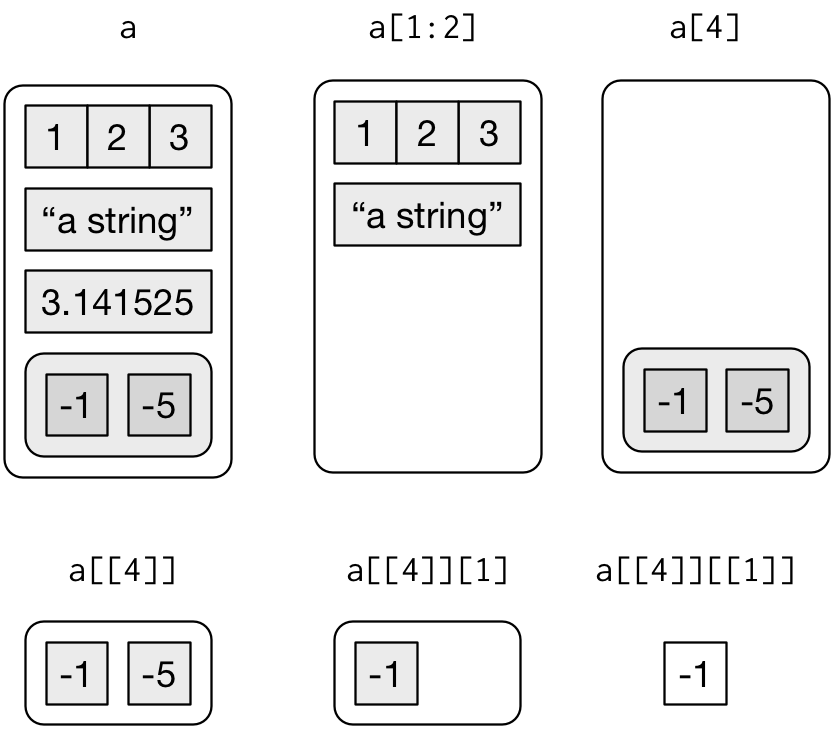
\includegraphics[width=2.97917in,height=\textheight]{images/ds-fp-list.png}

}

\caption{\label{fig-list-diagram}리스트에서 하위 리스트 뽑아내기 - 출처:
해들리 위컴}

\end{figure}%

범주형 자료를 R에 저장하기 위해서 요인(Factor) 클래스를 사용하며 요인
클래스를 사용하여 자료를 저장할 경우 저장 공간을 절약할 수 있다. 요인은
내부적으로 숫자(value)로 저장을 하고 레이블(value label)을 사용하여
표시하여 저장 공간을 절약한다. \index{범주형}

\begin{tcolorbox}[enhanced jigsaw, coltitle=black, breakable, opacityback=0, colback=white, bottomtitle=1mm, titlerule=0mm, toptitle=1mm, title=\textcolor{quarto-callout-note-color}{\faInfo}\hspace{0.5em}{자료형 확인}, left=2mm, rightrule=.15mm, colframe=quarto-callout-note-color-frame, bottomrule=.15mm, leftrule=.75mm, toprule=.15mm, arc=.35mm, colbacktitle=quarto-callout-note-color!10!white, opacitybacktitle=0.6]

각각의 데이터 형식에 맞는지를 다양한 테스트 함수(\texttt{is.})를
이용하여 데이터 형식을 확인할 수 있다.

\begin{itemize}
\tightlist
\item
  \texttt{is.list} : 리스트 형식인 확인
\item
  \texttt{is.factor} : 팩터 형식인지 확인
\item
  \texttt{is.numeric} : 숫자형인지 확인
\item
  \texttt{is.data.frame} : 데이터 프레임형인지 확인
\item
  \texttt{is.character} : 문자형인지 확인
\end{itemize}

\end{tcolorbox}

\section{자료형 확장}\label{extended-data-type}

요인, 텍스트, 날짜와 시간도 R에서 자주 사용되는 중요한 데이터 자료형으로
별도로 다뤄진다. 이를 위해서 \texttt{stringr}, \texttt{lubridate},
\texttt{forcats} 팩키지를 사용해서 데이터 정제 작업은 물론 기계학습
예측모형 개발에 활용한다.

\begin{figure}[H]

{\centering 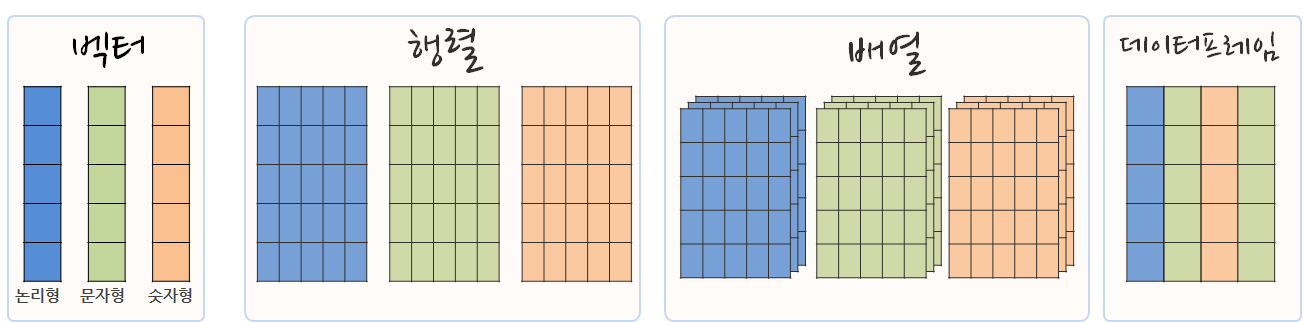
\includegraphics{images/ds-data-structure-pictogram.png}

}

\caption{데이터 과학 중요 자료구조}

\end{figure}%

\begin{longtable}[]{@{}ccc@{}}
\toprule\noalign{}
R 자료형 & 자료형 & 예제 \\
\midrule\noalign{}
\endhead
\bottomrule\noalign{}
\endlastfoot
\texttt{logical} & 부울 & 부도여부(Y/N), 남여 \\
\texttt{integer} & 정수 & 코로나19 감염자수 \\
\texttt{factor} & 범주 & 정당, 색상 \\
\texttt{numeric} & 실수 & 키, 몸무게, 주가, 환율 \\
\texttt{character} & 텍스트 & 주소, 이름, 책제목 \\
\texttt{Date} & 날짜 & 생일, 투표일 \\
\end{longtable}

\index{자료형!부울} \index{자료형!정수} \index{자료형!실수}
\index{자료형!텍스트} \index{자료형!날짜}

\section{범주 자료형}\label{data-type-factor}

명목척도 범주형, 서열척도 범주 자료형을 생성하는 경우 주의를 기울여야
한다. \texttt{factor} 함수를 사용해서 요인형 자료형을 생성하는데,
내부적으로 저장 공간을 효율적으로 사용하고 속도를 빠르게 하는 데
유용하다. 순서를 갖는 범주형의 경우 \texttt{factor} 함수 내부에
\texttt{levels} 인자를 넣어 정의하면 순서 정보가 유지된다.
\index{함수!factor}

\begin{Shaded}
\begin{Highlighting}[]
\NormalTok{\#| label: data{-}type{-}ordinal}
\NormalTok{\# 범주형 {-} 명목척도}
\NormalTok{animals\_vector \textless{}{-} c("Elephant", "Giraffe", "Donkey", "Horse")}
\NormalTok{factor\_animals\_vector \textless{}{-} factor(animals\_vector)}
\NormalTok{factor\_animals\_vector}

\NormalTok{\# 범주형 {-} 서열 척도}
\NormalTok{temperature\_vector \textless{}{-} c("High", "Low", "High","Low", "Medium")}
\NormalTok{factor\_temperature\_vector \textless{}{-} factor(temperature\_vector, order = TRUE, levels = c("Low", "Medium", "High"))}
\NormalTok{factor\_temperature\_vector}
\end{Highlighting}
\end{Shaded}

범주형 자료의 경우 범주가 갖는 척도 가독성을 높이기 위해
\texttt{levels()} 함수를 사용하기도 한다.

\begin{Shaded}
\begin{Highlighting}[]
\NormalTok{\#| label: data{-}type{-}factor{-}level}
\NormalTok{\# "M", "F" 수준}
\NormalTok{survey\_vector \textless{}{-} c("M", "F", "F", "M", "M")}
\NormalTok{factor\_survey\_vector \textless{}{-} factor(survey\_vector)}
\NormalTok{levels(factor\_survey\_vector)}

\NormalTok{\# "Female", "Male" 로 변환}
\NormalTok{levels(factor\_survey\_vector) \textless{}{-} c("Female", "Male")}
\NormalTok{levels(factor\_survey\_vector)}
\end{Highlighting}
\end{Shaded}

통계 처리와 자료분석에 문자형 벡터와 요인 범주형 벡터를 다른 의미를 갖는
점에 유의한다. 동일한 \texttt{summary()} 함수지만 입력 자료형에 따라 R은
적절한 후속 작업을 자동으로 수행한다.

\begin{Shaded}
\begin{Highlighting}[]
\NormalTok{\#| label: r data{-}type{-}factor{-}summary}
\NormalTok{\# 문자형 벡터와 요인 벡터}
\NormalTok{survey\_vector \textless{}{-} c("M", "F", "F", "M", "M")}
\NormalTok{factor\_survey\_vector \textless{}{-} factor(survey\_vector)}

\NormalTok{\# 문자형 벡터 요약}
\NormalTok{summary(survey\_vector)}

\NormalTok{\# 요인 벡터 요약}
\NormalTok{summary(factor\_survey\_vector)}
\end{Highlighting}
\end{Shaded}

\section{데이터프레임}\label{data-type-dataframe-in-r}

\textbf{R}은 6가지 기본 벡터로 자료를 저장하지만, 이외에 행렬(matrix),
데이터프레임(data.frame), 리스트(list) 자료구조가 있다. 하지만,
자료분석을 위해서 데이터를 데이터셋의 형태로 구성해야 한다. 데이터셋이
중요한 이유는 자료를 분석하기 위해서 다양한 형태의 개별 자료를
통합적으로 분석하기 위해서다. 이를 위해서 리스트 자료구조로 일단 모으게
된다. 예를 들어 개인 신용분석을 위해서는 개인의 소득, 부채, 성별, 학력
등등의 숫자형, 문자형, 요인(Factor)형 등의 자료를 데이터셋에 담아야
한다. 특히 변수와-관측값(Variable-Observation) 형식의 자료를 분석하기
위해서는 데이터프레임(\texttt{data.frame})을 사용한다. 데이터프레임은
모든 변수에 대해서 관측값이 같은 길이를 갖도록 만들어 놓은 것이다.
\index{자료형!데이터프레임} \index{자료형!리스트}

\begin{figure}[H]

{\centering 
\includegraphics[width=2.73958in,height=\textheight]{images/data-handling-list-dataframe.png}

}

\caption{리스트와 데이터프레임}

\end{figure}%

데이터프레임은 \texttt{data.frame()} 함수를 사용해서 생성한다. R 객체
구조 파악을 위해서는 간단한 자료의 경우 데이터 형식을 확인할 수 있는
1--2줄 정도의 간단한 스크립트와 명령어를 통해서 확인이 가능하지만,
복잡한 데이터의 구조를 파악하기 위해서는 \texttt{summary} 함수와
\texttt{str} 함수를 통해서 확인해야 한다.

\begin{Shaded}
\begin{Highlighting}[]
\NormalTok{\#| label: df{-}create}
\NormalTok{\# 벡터를 정의한다.}
\NormalTok{name \textless{}{-} c("Mercury", "Venus", "Earth", "Mars", "Jupiter", "Saturn", "Uranus", "Neptune")}
\NormalTok{type \textless{}{-} c("Terrestrial planet", "Terrestrial planet", "Terrestrial planet", }
\NormalTok{          "Terrestrial planet", "Gas giant", "Gas giant", "Gas giant", "Gas giant")}
\NormalTok{diameter \textless{}{-} c(0.382, 0.949, 1, 0.532, 11.209, 9.449, 4.007, 3.883)}
\NormalTok{rotation \textless{}{-} c(58.64, {-}243.02, 1, 1.03, 0.41, 0.43, {-}0.72, 0.67)}
\NormalTok{rings \textless{}{-} c(FALSE, FALSE, FALSE, FALSE, TRUE, TRUE, TRUE, TRUE)}

\NormalTok{\# 벡터를 합쳐서 데이터프레임을 생성}
\NormalTok{planets\_df \textless{}{-}data.frame(name, type, diameter, rotation, rings)}
\end{Highlighting}
\end{Shaded}

\section{벡터, 행렬, 배열, 데이터프레임}\label{data-type-vector}

가장 많이 사용되는 논리형, 문자형, 숫자형을 통해 자료분석 및 모형개발을
진행하게 되고, 경우에 따라서 동일한 자료형을 모은 경우 이를 행렬로
표현할 수 있고, 행렬을 모아 RGB 시각 데이터를 위한 배열(Array)로
표현한다. 데이터프레임은 서로 다른 자료형을 모아 넣은 것이다.
\index{자료형!벡터} \index{자료형!행렬} \index{자료형!배열}
\index{자료형!데이터프레임}

\begin{figure}[H]

{\centering 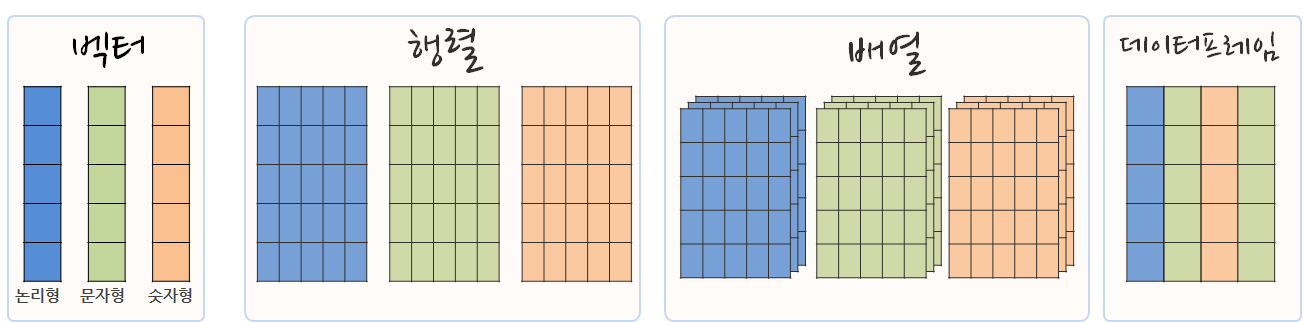
\includegraphics[width=1\textwidth,height=\textheight]{images/ds-data-structure-pictogram.png}

}

\caption{R 자료구조 - 벡터, 행렬, 배열, 데이터프레임}

\end{figure}%

\section{\texorpdfstring{\texttt{NULL}과
\texttt{NA}}{NULL과 NA}}\label{is-na-null}

결측되었다는 없다는 것을 표시하는 방법이 두 가지 필요하다. 하나는 벡터가
없다는 \texttt{NULL}이고, 벡터 내부에 값이 결측되었다는 \texttt{NA}다.
\texttt{dataframe\$variable\ \textless{}-\ NULL} 명령문을 사용하면
데이터프레임(\texttt{dataframe})에 변수(\texttt{variable})를 날려보내는
효과가 있다. 예를 들어 책장이 아예 없다는 의미(\texttt{NULL})와 책장에
책이 없다(\texttt{NA})는 다른 개념을 지칭하고 쓰임새가 다르다.
\index{자료형!NULL} \index{자료형!NA}

\textbf{\texttt{NULL}}

\begin{Shaded}
\begin{Highlighting}[]
\CommentTok{\# NULL 자료형과 길이}
\FunctionTok{typeof}\NormalTok{(}\ConstantTok{NULL}\NormalTok{)}
\CommentTok{\#\textgreater{} [1] "NULL"}
\FunctionTok{length}\NormalTok{(}\ConstantTok{NULL}\NormalTok{)}
\CommentTok{\#\textgreater{} [1] 0}
\end{Highlighting}
\end{Shaded}

\textbf{\texttt{NA}}

\begin{Shaded}
\begin{Highlighting}[]
\CommentTok{\# NA 자료형과 길이}
\FunctionTok{typeof}\NormalTok{(}\ConstantTok{NA}\NormalTok{)}
\CommentTok{\#\textgreater{} [1] "logical"}
\FunctionTok{length}\NormalTok{(}\ConstantTok{NA}\NormalTok{)}
\CommentTok{\#\textgreater{} [1] 1}
\end{Highlighting}
\end{Shaded}

\texttt{NA}의 중요한 특징은 전염된다는 것이다. 즉, \texttt{NA}에 연산을
가하면 연산 결과는 무조건 \texttt{NA}가 된다. \texttt{NA}가 7보다 큰지,
7을 더하고 빼고, 부울 연산을 하든 \texttt{NA}와 연산 결과는 무조건
\texttt{NA}가 된다.

\begin{Shaded}
\begin{Highlighting}[]
\ConstantTok{NA} \SpecialCharTok{+} \DecValTok{7}
\CommentTok{\#\textgreater{} [1] NA}
\ConstantTok{NA} \SpecialCharTok{/} \DecValTok{7}
\CommentTok{\#\textgreater{} [1] NA}
\ConstantTok{NA} \SpecialCharTok{\textgreater{}} \DecValTok{7}
\CommentTok{\#\textgreater{} [1] NA}
\DecValTok{7} \SpecialCharTok{==} \ConstantTok{NA}
\CommentTok{\#\textgreater{} [1] NA}
\ConstantTok{NA} \SpecialCharTok{==} \ConstantTok{NA}
\CommentTok{\#\textgreater{} [1] NA}
\end{Highlighting}
\end{Shaded}

\section{리스트 칼럼}\label{fp-list-columns}

레고를 통해 살펴본 R 자료구조는 계산 가능한 원자 자료형(논리형, 숫자형,
요인형)으로 크게 볼 수 있다. R에서 정수형과 부동소수점은 그다지 크게
구분을 하지 않는다. 동일 길이를 갖는 벡터를 쭉 붙여넣으면 자료구조형이
\textbf{데이터프레임}으로 되고, 길이가 같지 않는 벡터를 한 곳에 모아넣은
자료구조가 \textbf{리스트}다. \footnote{\href{https://jennybc.github.io/purrr-tutorial/ls13_list-columns.html}{List
  columns}} \footnote{\href{https://github.com/jennybc/lego-rstats}{Photos
  that depict R data structures and operations via Lego}}
\index{자료형!리스트 칼럼}

데이터프레임이 굳이 모두 원자벡터만을 갖출 필요는 없다. 리스트를
데이터프레임 내부에 갖는 것도 데이터프레임인데 굳이 구별하자면
티블(\texttt{tibble})이고, 이런 자료구조를
\textbf{리스트-칼럼(list-column)}이라고 부른다.

\begin{figure}

\centering{

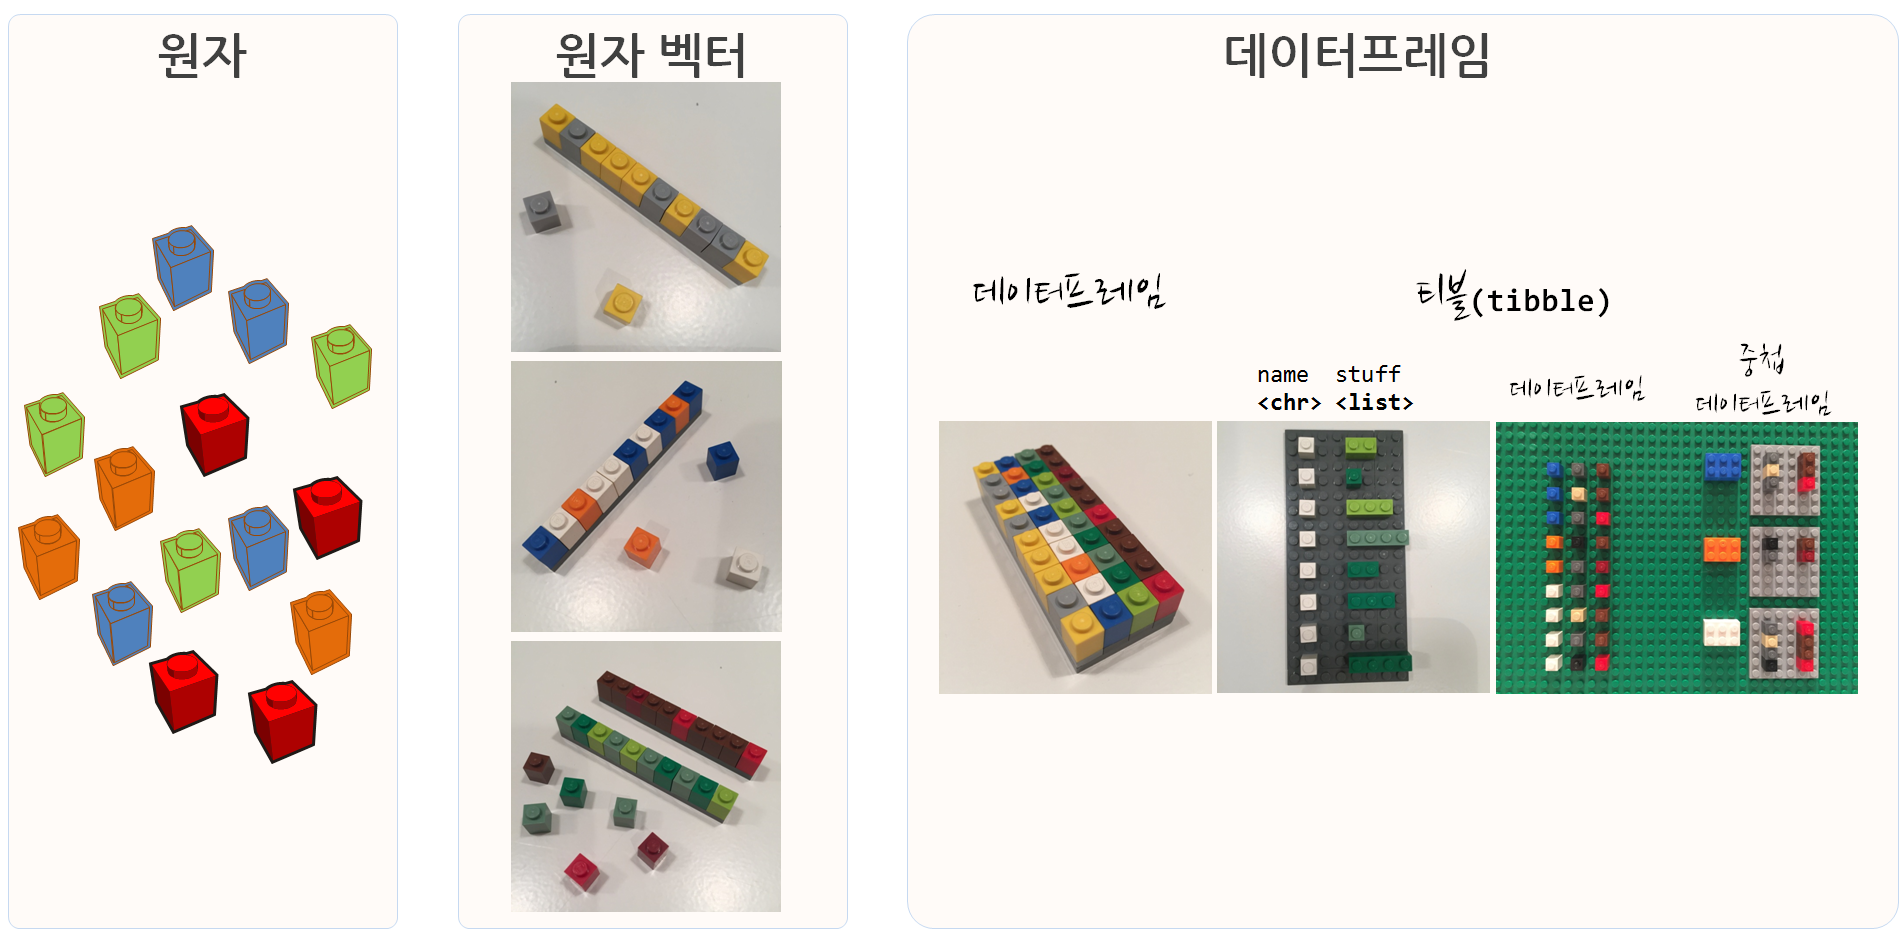
\includegraphics[width=1\textwidth,height=\textheight]{images/data-structure-list-column.png}

}

\caption{\label{fig-dataframe-list-columns}리스트 칼럼}

\end{figure}%

의외로 리스트-칼럼 자료구조를 실무에서 빈번히 마주하게 된다.
정규표현식을 사용하여 텍스트 데이터에서 원하는 패턴을 추출하거나 변환할
수 있다. 추출된 결과는 주로 리스트 형태로 저장되며, 리스트-칼럼을
활용하면 텍스트 처리 결과를 데이터프레임에 직접 저장할 수 있어 편리하다.
웹 API를 통해 수집한 JSON이나 XML 형식의 데이터는 계층적 구조를 가지고
있어 리스트-칼럼을 사용하여 데이터프레임에 저장하면 복잡한 구조의
데이터를 분석에 용이한 형태로 환하기 수월하다.

분할-적용-병합(Split-Apply-Combine) 전략은 데이터를 그룹별로 나누어 각
그룹에 동일한 연산을 적용하고, 결과를 다시 병합하는 방법으로 그룹별 연산
결과는 리스트 형태로 저장되며, 리스트-칼럼을 사용하여 데이터프레임에
통합시킨 후 후속 작업을 이어나가는 패턴을 흔히 볼 수 있다.

이렇게 리스트-칼럼을 활용하여 데이터를 처리하고 분석하는 과정에서,
티블(\texttt{tibble}) 형태의 데이터프레임을 사용하면 데이터 탐색과
조작이 한결 수월해진다. 데이터프레임이 티블(tibble) 형태로 되어 있을 때,
데이터프레임 파악, 인덱싱, 연산, 간략화 등 다양한 작업을 수월하게 할 수
있다.

먼저, 들여다보기(Inspect) 측면에서 티블 형태 데이터프레임은 콘솔에
출력했을 때 깔끔하게 보여주므로, 데이터의 구조와 내용을 쉽게 파악할 수
있다. 또한, \texttt{glimpse()} 함수를 사용하면 데이터프레임 개요를
자료형과 함께 한 눈에 확인할 수 있다.

인덱싱(Indexing) 측면에서는 티블이 데이터프레임과 동일하게
\texttt{{[}{]}}, \texttt{{[}{[}{]}{]}}, \texttt{\$} 연산자를 사용하여
원소에 접근할 수 있어, 열 이름이나 위치를 사용하여 원하는 변수나
관측값을 추출할 수 있다.

연산(Compute) 측면에서도 리스트-칼럼을 포함한 티블에서
\texttt{mutate()}, \texttt{summarise()} 등의 함수를 사용하여 새로운
변수를 생성하거나 요약 통계량을 계산할 수 있으며, 이 과정에서
리스트-칼럼에 대한 연산도 자연스럽게 수행할 수 있다.

마지막으로 간략화(Simplify) 측면에서는 리스트-칼럼을 포함한 티블을
일반적인 데이터프레임으로 변환할 때, \texttt{unnest()} 함수를 사용할 수
있다. 이를 통해 리스트-칼럼의 각 요소를 개별 행으로 풀어내어, 분석에 더
용이한 형태로 만들 수 있다.

\section*{연습문제}\label{uxc5f0uxc2b5uxbb38uxc81c-3}
\addcontentsline{toc}{section}{연습문제}

\markright{연습문제}

\subsection*{객관식}\label{uxac1duxad00uxc2dd}
\addcontentsline{toc}{subsection}{객관식}

\begin{enumerate}
\def\labelenumi{\arabic{enumi}.}
\tightlist
\item
  R에서 벡터 자료형을 주로 어떻게 분류하는가?
\end{enumerate}

\begin{enumerate}
\def\labelenumi{\alph{enumi})}
\tightlist
\item
  원자 벡터와 리스트
\item
  숫자형과 문자형
\item
  정수형과 실수형
\item
  행렬과 배열
\end{enumerate}

\begin{enumerate}
\def\labelenumi{\arabic{enumi}.}
\setcounter{enumi}{1}
\tightlist
\item
  데이터프레임에서 특정 변수를 제거하기 위해 사용하는 코드는?
\end{enumerate}

\begin{enumerate}
\def\labelenumi{\alph{enumi})}
\tightlist
\item
  dataframe\$variable == NULL
\item
  dataframe\$variable = NULL\\
\item
  dataframe\$variable \textless- NULL
\item
  dataframe \textless- NULL
\end{enumerate}

\begin{enumerate}
\def\labelenumi{\arabic{enumi}.}
\setcounter{enumi}{2}
\tightlist
\item
  다음 중 리스트-칼럼 자료구조를 활용하기에 적합하지 않은 경우는?
\end{enumerate}

\begin{enumerate}
\def\labelenumi{\alph{enumi})}
\tightlist
\item
  정규표현식을 통한 텍스트 문자열 처리
\item
  웹 API로 추출된 JSON, XML 데이터
\item
  분할-적용-병합(Split-Apply-Combine) 전략
\item
  단순한 숫자형 벡터 저장
\end{enumerate}

\subsection*{서술형}\label{uxc11cuxc220uxd615}
\addcontentsline{toc}{subsection}{서술형}

\begin{enumerate}
\def\labelenumi{\arabic{enumi}.}
\setcounter{enumi}{3}
\tightlist
\item
  데이터프레임을 생성하는 함수의 이름과 사용 예시를 간단히 작성하시오.
\end{enumerate}

\begin{enumerate}
\def\labelenumi{\arabic{enumi}.}
\setcounter{enumi}{4}
\tightlist
\item
  리스트-칼럼 자료구조의 장점을 설명하고, 이를 분석에 활용하는 방법에
  대해 서술하시오.
\end{enumerate}

\bookmarksetup{startatroot}

\chapter*{참고문헌}\label{uxcc38uxace0uxbb38uxd5cc}
\addcontentsline{toc}{chapter}{참고문헌}

\markboth{참고문헌}{참고문헌}

\printbibliography[heading=none]


\backmatter


\printindex

\end{document}
